\documentclass{article}

\usepackage[style=authoryear, backend=biber]{biblatex}
\addbibresource{references.bib}
\addbibresource{method.bib}
\usepackage[a4paper, total={6 in, 9 in}]{geometry}

\usepackage{mathtools}
\usepackage{graphicx}
\usepackage{subcaption}
\usepackage{caption}
\usepackage{booktabs}
\usepackage{adjustbox}
\usepackage{multirow}
\usepackage{caption}
\usepackage{eurosym} 
\usepackage{xcolor}
\usepackage{comment}
\usepackage{subcaption}
\usepackage{amssymb, amsmath}
\usepackage{algorithm}
\usepackage{algpseudocode}
\usepackage{blindtext}
\usepackage{pdflscape}
\usepackage{rotating}
\usepackage{longtable}
\usepackage{placeins}
\usepackage{spverbatim}
\usepackage{tikz}
\usepackage{rotating}
\usepackage{pgfplots}
\pgfplotsset{width=10cm,compat=1.9}

\usepackage{makecell}
\usepackage[flushleft]{threeparttable}
\renewcommand\theadalign{bc}
\renewcommand\theadfont{\bfseries}
\renewcommand\theadgape{\Gape[4pt]}
\renewcommand\cellgape{\Gape[4pt]}
\usepackage{tikz}
\usepackage{tikz-3dplot}

\usetikzlibrary{shapes,shapes.geometric, positioning, fit, backgrounds, calc, 3d, shapes.multipart, arrows.meta, patterns, perspective}

\newcommand\lbo{0.5}
\newcommand\wbo{1}
\newcommand\hbo{1}
\newcommand\lbt{2}
\newcommand\wbt{1}
\newcommand\hbt{1}
\newcommand\separationofcircles{0.1}


\tikzset{
    single_redbox/.pic={
    \draw[red, dashed, opacity=0.5] (0-\lbo,0-\wbo,0-\hbo) -- ++(0,0,\hbo);
    \draw[red, dashed, opacity=0.5] (0-\lbo,0-\wbo,0-\hbo) -- ++(0,\wbo,0);
    \draw[red, dashed, opacity=0.5] (0-\lbo,0-\wbo,0-\hbo) -- ++(\lbo,0,0);
    
    % Draw front faces
    \draw[red, fill=red!20, opacity=0.5] (0,0,0) -- ++(-\lbo,0,0) -- ++(0,-\wbo,0) -- ++(\lbo,0,0) -- cycle;
    \draw[red, fill=red!30, opacity=0.5] (0,0,0) -- ++(0,0,-\hbo) -- ++(0,-\wbo,0) -- ++(0,0,\hbo) -- cycle;
    \draw[red, fill=red!40, opacity=0.5] (0,0,0) -- ++(-\lbo,0,0) -- ++(0,0,-\hbo) -- ++(\lbo,0,0) -- cycle;
    }
}
\tikzstyle{line} = [draw, -Latex]

\newcommand{\neworrenewcommand}[1]{\providecommand{#1}{}\renewcommand{#1}}

\newcommand{\drawblock}[9]{
    \neworrenewcommand{\ffoo}[1]{
           
        \foreach \i in {0,...,#8} {
            \foreach \j in {0,...,#9} {
                \foreach \k in {0,...,##1} {
                    % Only draw the visible faces
                    % Front face
                    \ifnum \i=#8
                        \draw[#7, fill=#7!50] (#1+\i*#4+#4,#2+\j*#5,#3+\k*#6) -- ++(0,#5,0) -- ++(0,0,#6) -- ++(0,-#5,0) -- cycle;
                    \fi
                    % Right face
                    \ifnum \j=#9
                        \draw[#7, fill=#7!30] (#1+\i*#4,#2+#5+\j*#5,#3+\k*#6) -- ++(#4,0,0) -- ++(0,0,#6) -- ++(-#4,0,0) -- cycle;
                    \fi
                    % Top face
                    \ifnum \k=##1
                        \draw[#7, fill=#7!20] (#1+\i*#4,#2+\j*#5,#3+#6+\k*#6) -- ++(#4,0,0) -- ++(0,#5,0) -- ++(-#4,0,0) -- cycle;
                    \fi
                    % Draw a point at each vertex
                    % \fill (#1+\i*#4,#2+\j*#5,#3+\k*#6) circle (1pt);
                }
            }
        }
    
    }
    \ffoo
}



      \tikzset{
    box/.style={rectangle, draw, fill=gray!20, align=center, minimum height=1cm, minimum width=2.5cm},
    ellip/.style={draw, ellipse, align=center, minimum width=2.5cm, minimum height=1cm},
    label_node/.style={circle, draw, fill=#1, text=black, inner sep=1pt, minimum size=1em, font=\bfseries},
    gene_node/.style={ align=center, inner sep=2pt, fill=white, minimum width=0.5cm, minimum height=1cm},
    gene_group/.style={rectangle, draw, inner sep=6pt, rounded corners, align=center, minimum height=2.5cm},
    aux_gene_group/.style={align=center, inner sep=2pt, minimum width=2cm, minimum height=1cm}
  }


% Same options as configuraciones/paquetes_comunes.tex, which loads acronym
% first in the thesis: a second load with other options clashes.
\usepackage[printonlyused,nolist]{acronym}
\providecommand{\keywords}[1]
{
  \small	
  \textbf{\textit{Keywords---}} #1
}

% Visible marker for a number or table that does not exist yet.  Every use is
% a place where a generated fragment or a regenerated run must supply the
% value; grep for \pending before submitting.
\providecommand{\pending}[1]{\textcolor{red}{\textbf{[pending: #1]}}}
\providecommand{\pendingcell}{\textcolor{red}{\textbf{[pending]}}}
\usepackage{amsthm}
\newtheorem{proposition}{Proposition}


% Text still awaiting a decision or a result (purple); listed in
% CHANGES-final3d.md, "Pending (purple)".
\providecommand{\Pending}[1]{\textcolor{purple}{#1}}
\usetikzlibrary{decorations.pathreplacing}
% Some long reference titles leave no good break at this width.
\AtBeginBibliography{\emergencystretch=2em}

\title{An optimisation approach for supply chain procurement transport
operational planning with 3D full-truckload constraints and returnable
transport items}
\date{}

\newenvironment{ChapterAppendix}{\appendix}{}

\begin{document}
\maketitle

% The manuscript's body; Renderer.tex holds the preamble and the bibliography.

% In the thesis, earlier chapters have already used some acronyms; start afresh.
\acresetall
% Base: old/main.tex lines 1-3 (the initial manuscript's abstract and keywords).
% Final ladder: results/julia/final/ladder_3d_final.csv (trucks 12-156, complaints 0,
% time_limit 900-3600, gap_pct 0.0075 / 0.1628 / 0.022 / 14.5186 / 10.686); minimum
% fleets on rungs 1-3 (5, 10, 12 periods): requirement prunes, ladder_3d_final.log
% lines 15, 651, 705.  Volumetric stage: Table tab:volumetric (results/julia/
% parity_vol.csv against results/compact_ref/*.json): 68139.21 vs 68139.17
% (0.0001%), certified bound 0.0113% below, four memory-stop rows within 0.31%.
% Benchmark: results/julia/final/bench36/bench36_joined.csv (branch final-3d,
% 360c2ea): 32 rows with method_cost, median gap_pct 6.4642 against best_lb;
% bench36_method.csv complaints 0 and pack_undecided 0 on every row.
% Volumetric plans: Table tab:repack and census_compact36.json (unplaceable
% loads on 35 of 36 plans).
% Catalogue: results/catalogue_realism.json (kappa: nine at 1.000, two at 1.176,
% four at 1.231-2.000, so six of fifteen above 1).
% Words: 239 from the PDF with "3 600" as one word (240 as two).
We propose a mixed integer linear programming model, 3D-SCPTOP, for procurement transport planning, integrating procurement, inventory and transport decisions of a plant and its supplier with three-dimensional full-truckload constraints and closed-loop management of returnable transport items. We reformulate it by Dantzig--Wolfe decomposition, with the loaded truck as the unit of decision: every geometric, stacking, crush, payload and full-truckload constraint lives inside one pricing problem per direction, and a column keeps its layout, so plans are executable by construction. The master is solved by branch and price over the fleet vector with a flow-first relax-and-fix construction as primal heuristic, and a certified volumetric bound is a valid lower bound for the 3D problem. On the volumetric problem the method returns a plan $0.0001\%$ above a proved optimum. On the 3D problem, where the compact model returns no incumbent beyond five periods, it returns verified plans on all five instances of a ladder reaching twenty-four products and twenty periods, from $12$ to $156$ trucks within $900$ to $3\,600$ s, with provably minimum fleets through twelve periods and gaps to its certified bound of $0.0075\%$ to $0.163\%$, and $14.5\%$ and $10.7\%$ where a per-stack crush limit binds. On a 36-instance benchmark it returns $32$ verified plans, at a median gap of $6.46\%$ to the best valid bound. Volumetric plans prescribe loads proved impossible to place, so a volumetric capacity is not a conservative simplification: it over-credits six of fifteen industrial container types.

\keywords{ Procurement, inventory, transport planning,  full-truckload, 3D container loading }

% The abstract stands alone: the body defines each acronym again at its first use.
\acresetall
\section{Introduction}
\label{sec:intro}

Optimizing the use of resources in manufacturing supply chains is crucial for boosting economic growth, improving social well-being, and minimizing environmental impact.
Integrating transport, inventory, and production processes is a fundamental characteristic of supply chains \autocite{Stadtler2015SupplyPlanning} because joint decisions will improve supply chain performance\autocite{Diaz-Madronero2017ADecisions}.

Procurement refers to the process of acquiring goods and services in a supply chain \autocite{Chopra2015SupplyOperation}.
One of the main goals of procurement is to obtain \ac{RM}, parts or \ac{FG} for a factory or distribution centre from a supplier.
As mentioned in \autocite{Fleischmann2015TransportDistribution}, the responsibility for transport planning usually lies with the supplier.
However, on some \acp{SC}s the manufacturer makes transport decisions of its supplies in, for example, the automotive industry.
Furthermore, an essential asset in the automotive supply chain is not always considered in traditional \ac{MRP}: returnable containers or \acfp{RTI}, which are used as tertiary packaging.
\acp{RTI} enable the storage and transportation of \ac{RM} and \ac{FG} through the supply chain.
Usually, the manufacturing plant supplies empty \acp{RTI} to its supplier, while the supplier delivers full \acp{RTI} with the \ac{FG} or \ac{RM}.
Therefore, during the procurement process, transport and inventory decisions should be integrated, including \ac{RTI} management.
Here, we focus on optimising the operational decisions made during procurement transport planning.

According to \autocite{Diaz-Madronero2014AChain}, using algorithm-based methods for procurement transport planning is more efficient than relying on manual approaches based on planners' intuition.
Manual planning can be short-sighted and lead to less efficient outcomes.
This becomes even more significant when optimizing procurement transport tasks that aim to reduce the number of trucks and inventory levels, especially under 3D loading constraints where the precise placement of containers within trucks must also be determined.
Furthermore, the capacity constraints used in the scientific literature on procurement transport planning are based mainly on freight volume or the total number of loaded product units {\autocite{Hashemi-Amiri2023IntegratedApproach} and \autocite{Diaz-Madronero2014AChain}.
	}
The current research seeks to address this gap by introducing a new \ac{MILP} model.
This model uniquely combines procurement transportation with 3D full-truck loading, inventory management, and \ac{RTI} management.
Hereafter, we refer to this model as the \ac{RTISC}, and to its volumetric relaxation, in which truck capacity is a volume limit, as the \ac{VRTISC}.
Additionally, a \ac{BP} procedure is developed to solve both, and it is compared against the \ac{CF} solved directly by Gurobi, a commercial solver.

In this paper, we present four main contributions:
(i) We formulate a novel \ac{MILP} model, the \ac{RTISC}, integrating procurement transport, \ac{RTI} management and inventory decisions with stack-based full-truck loading constraints.
(ii) We use \ac{DW} decomposition to reformulate the problem over 3D loading configurations per time period. We define a \ac{BP} schema with column generation over that mixed integer pricing problem and a relax-and-fix construction as primal heuristic, giving the \ac{RTISCBP}.
(iii) We validate the accuracy of the \ac{BP} procedure against the \ac{CF} on both the 3D loading problem and its volumetric relaxation.
On the \ac{VRTISC}, where the \ac{VRTISCCF} reaches a proved optimum, the \ac{VRTISCBP} matches it to within $0.0001\%$ (Section~\ref{sec:res-vol}).
{\color{red} Comentar difencias entre BP y CF para el 3d}.
(iv) We show that the \ac{VRTISC}, the volumetric representation of truck capacity used in the procurement transport literature, yields plans that are cheaper on paper but cannot be loaded in practice, nor repaired by re-packing their own quantities.
{\color{red} Añadir algo vs company procedures}.

Readers are referred to the typology by \autocite{Wascher2007AnProblems} for a global view of container loading problems, where the different dimensions of the loading problem are described.
Furthermore, \autocite{Silva2019ExactProblems} summarise the exact methods used in the literature to solve container loading problems, and \autocite{Zhao2016INTERNATIONALAlgorithms} explore other solution approaches in the literature.
Readers are also referred to the literature reviews of \autocite{Mosca2019IntegratedReview} and \autocite{Diaz-Madronero2015ADecisions}, which focus more on integrating inventory decisions and transport.
Here, we jointly address container loading, procurement transport and inventory decisions.

The paper is organised as follows.
Section~\ref{sec:lit} provides a literature review related to the problem under study.
Section~\ref{sec:problem} presents the problem description.
Section~\ref{sec:model} describes the \ac{RTISC} \ac{MILP} formulation.
Sections~\ref{sec:decomp}--\ref{sec:branching} develop the \ac{BP} solution approach, the \ac{RTISCBP}, together with its pricing subproblem and bounding arguments.
Section~\ref{sec:results} reports the computational experiments.
Finally, Section~\ref{sec:conclusions} concludes and puts forward further research lines.

\section{Literature Review}
\label{sec:lit}

The goal of this research is to integrate procurement transport operational planning decisions with 3D loading restrictions and RTI packaging. Based on the authors’ research, no previous work has been identified that meets this criterion. Therefore, three independent, but sometimes overlapping, knowledge bodies have been reviewed: procurement transport and inventory planning, container loading problems and RTI literature.

\subsection{Procurement transport and inventory planning}

Models that integrate transport and inventory costs during the procurement process are widely studied in the literature. As noted in \autocite{Langley2020SupplyPerspective}, transportation facilitates the movement of raw materials and finished products between suppliers,  warehouses, manufacturers, and retailers. Therefore, transport processes play a crucial role in supply chains. \autocite{Fleischmann2015TransportDistribution} distinguish between two main types of transportation within a supply chain: "procurement transport," which involves moving materials from suppliers to manufacturing sites, and the "distribution of goods," which concerns delivering finished products from factories to customers. This article focuses specifically on addressing the challenges related to procurement transportation.

There are two main dimensions of procurement transport problems according to the supply chain configuration and the applied transport method. Regarding supply chain configurations \autocite{Mosca2019IntegratedReview}: (i) single source to a single destination (SS); (ii) multiple sources to a single destination (MS);
(iii) single source to multiple destinations (SM); (iv) multiple sources to multiple destinations (MM). Source components determine the number of supplier locations that are taken into account, while destination components denote the number of supplied manufacturers. Additionally, different transport methods are identified in \autocite{Diaz-Madronero2014AChain}:milk run, less-than-truckload (LTL),  full-truckload (FTL) . We also analyze the formulation of the transportation capacity constraints in the scientific literature.

\autocite{Berman2006InboundCost} address the problem of optimising distribution strategies to deliver products from suppliers to plants, whose aim is to minimise transport, pipeline and plant inventory costs by using cross docks. A mixed integer non-linear programming (MINLP) formulation, a Lagrangian  relaxation heuristic,  a greedy heuristic, and a branch-and-bound algorithm are proposed to model and solve the problem.

\autocite{Sancak2011Multi-itemPolicy} present a MILP model to optimise procurement transport decisions in a SS supply chain configuration using LTL and FTL transport methods. The objective is to minimise transport and inventory holding costs, while fulfilling production plan requirements on a multiperiod planning horizon. The study explores the possibility of delaying LTL shipments to the subsequent time period, and utilising safety stocks whenever necessary, in a stochastic environment by employing data from a bus manufacturer. The findings demonstrate that delaying shipments leads to reduced holding and transport costs with a minimal stockout risk.


\autocite{Schoneberg2010AnNetworks} examine the concept of delivery profiles, which define the delivery frequency at a fixed rate, offering structured planning, minimizing management effort, and improving coordination in logistics. In this context, FTL transport is used when the goods' volume exceeds a vehicle's capacity, making direct shipment possible. LTL is applied when the volume is insufficient to fill a truck, and the goods are first sent to a consolidation center before reaching the final destination. In \autocite{Schoneberg2013ANetworks}, the proposed model accounts for demand uncertainty.

\autocite{Diaz-Madronero2014AChain} present a  fuzzy  multi-objective  integer  linear programming (FMOILP) model that focuses on operational procurement transport planning in an automotive supply chain, which involves a single source and a single destination while utilising FTL. The developed model aims to minimise the number of trucks employed for procurement transport and the inventory level by considering the uncertainties related to transport capacity levels.

\autocite{Hein2016QuantitativeProblem} investigate the benefits of integrated procurement transport and production planning for supply and production processes by comparing a sequential approach, where production is firstly determined, followed by procurement transport decisions, plus an integrated approach in which decisions are jointly made. Numerical experiments reveal that the integrated planning approach leads to substantial cost savings.

\autocite{Diaz-Madronero2017ADecisions} present an novel MILP model that integrates  procurement, production and transport planning decisions within manufacturing systems. This model extends beyond traditional material requirement planning (MRP) systems by incorporating procurement transport decisions from multiple sources and a single destination into a unified optimization framework. It considers the capacities of both material and production resources, along with procurement transport planning decisions, by employing various shipping modes such as FTL, LTL, and milk-run.

\autocite{Chitsaz2019ARouting} address integrating production, inventory and procurement transport into a manufacturing context by defining this problem as an assembly routing problem (ARP). It introduces a novel MILP model for the ARP and proposes a three-phase decomposition matheuristic for its solution.

\autocite{Baller2022OptimizingApproach} examine the optimization of procurement transport in an automotive factory, focusing on first-tier suppliers at an aggregate level across multiple sources (570) to a single destination, using FTL, LTL, and courier express service (CES) as transportation methods. The proposed MILP approach includes a cyclic inventory constraint, truck utilization, and storage limitations.

\autocite{Hashemi-Amiri2023IntegratedApproach} propose an integrated approach to optimize a perishable food supply chain. The model combines supplier selection, procurement and distribution transport, production scheduling, and vehicle routing to improve supply chain efficiency and resilience. It handles demand uncertainties through a distributionally robust chance-constrained model. The model is reformulated as MILP by utilizing duality and linearization techniques.


\subsection{Procurement Transport with RTIs}
Some models further integrate the procurement and delivery of RTIs into the procurement transport literature. In this sense, RTIs are procured to the supplier, who loads the items and sends them to customer. We extend the supply chain definitions previously defined to contemplate the RTIs management strategies.

% TODO(author): ACTION REQUIRED BEFORE THIS PARAGRAPH IS RESTORED.
% The paragraph below has no subject and no citation: the work it describes --- a
% food closed-loop supply chain network design problem with RTIs, product
% perishability, facility location and demand uncertainty, a two-stage non-linear
% chance-constrained model linearised by sample average approximation, solved by
% an improved Lagrangian relaxation that beats CPLEX --- is not identifiable from
% anything in references.bib (the nearest entry, Zhang17012024, is a closed-loop
% inventory ROUTING problem with RTI selection, not network design, and uses no
% Lagrangian relaxation).  A referee flagged it as typeset without a citation;
% commenting it out answers that, because an uncited paragraph in the literature
% review is worse than a shorter literature review.  To restore it: supply the
% reference, open the paragraph with \autocite{...}, and give it a subject.
%
% Model a food closed-loop supply chain network design problem incorporating returnable transport items (RTIs), product perishability, facility location and demand uncertainty. A two-stage non-linear chance-constrained programming model minimizes fixed facility, production, transport, inventory holding and RTI costs while ensuring a target service level. It's linearized via sample average approximation and distribution-free methods to capture forward RTI-based shipments and reverse flows for reuse. To solve large instances, an improved Lagrangian relaxation algorithm decomposes facility-location and flow decisions, outperforming CPLEX on solution quality and speed.


\autocite{SOYSAL2023101504} develop a tactical-level, multi-period closed-loop Vendor-Managed Inventory (VMI) system for RTIs in an agro-food supply chain. The SM supply chain integrates forward flows of full RTIs from a single vendor to multiple customers and reverse flows of empties back to the vendor for cleaning . All routing and inventory decisions are made centrally by the vendor under full information sharing. Sustainable plans in terms of amounts of energy spent and empty crates collected are devised and evaluated.


\autocite{GUO2024104339} model two-tier Container Management Centre (CMC) network . Empty RTIs are dispatched from central CMC hubs to upstream suppliers, loaded with products, carried by truck to downstream customers, then returned empty to regional CMCs for cleaning and storage before being shipped back to central hubs. A neural network is used for demand forecasting. A MILP is proposed that maximises total profit by optimally determining transport costs and the penalties applied to late RTIs returns.


\autocite{Zhang17012024} formulate a perishable-food inventory-routing MILP with multiple RTI types in a SM supply chain, integrating procurement of products and pickup of both filled and empty RTIs. Decisions are made on a operational level, optimally determining per period the quantities to pack, deliver, pick up, purchase and lose, as well as the vehicle routes in order to maximise the total profit of the supply chain that is equal to the total quality-dependent revenue minus the total costs involved, including inventory holding costs, product cost, transportation costs, and RTI purchasing and loss costs. The model is solved exactly via CPLEX  solver and approximately via a tailored Kernel Search matheuristic.


\subsection{Container loading}

Container loading problems encompass a subset of geometric assignment problems known as cutting and packing ($C\&P$) problems. They revolve around the allocation of n-dimensional orthotope items in larger n-dimensional orthotope containers. Here the aim is to optimise an objective function while taking into account two key geometric constraints: complete containment of items inside containers and lack of item overlap. A loading pattern serves as a formal representation of a solution to such an assignment problem.
Dyckhoff introduced in \autocite{Dyckhoff1990AProblems} a typology that unifies $C\&P$ problems using four different criteria: dimensionality of space, the objective of assignment, containers types and box type. Consequently, \autocite{Wascher2007AnProblems} develop a new typology that has become the standard in the $C\&P$ literature. We   briefly  describe  the  typology  used  in  \autocite{Wascher2007AnProblems}  based  on  five different criteria: (i) dimensionality of space; (ii) kind of assignment (input minimisation of containers for all small items and loading patterns; output maximisation to pack a subset of small items with limited container availability;) (iii) assortment of small item by distinguishing if they are either a weakly (or strongly) heterogeneous assortment or identical small items ; (iv) assortment of large objects (if it is either several large objects or one large object); (v) shape of small items (circular or of another shape). In that typology's names, the problems cited below are the single large object placement problem (SLOPP), the multiple identical large object placement problem (MILOPP) and the single knapsack problem (SKP) on the output-maximisation side, and the single stock size cutting stock problem (SSSCSP), the multiple stock size cutting stock problem (MSSCSP) and the single and multiple bin size bin packing problems (SBSBPP, MBSBPP) on the input-minimisation side; 3D-BPP is the three-dimensional bin packing problem.





The first mathematical programming model in a scientific journal to describe the container-loading problem was developed in \autocite{Chen1995EUROPEANProblem}, where the authors introduced an MILP model to address the 3D  input minimisation problem by considering rotations and containers of varying dimensions. However, it does not specify the use of weakly or strongly heterogeneous boxes or containers. Additionally, real-world constraints are modelled like, for example, weight distribution.

\autocite{Junqueira2012Three-dimensionalConstraints} propose an alternative MILP formulation to \autocite{Chen1995EUROPEANProblem} using binary encoding for box position, which utilises normal patterns to reduce possible box coordinates by considering multiples of boxes dimensions and ensuring optimal solutions. Additionally, loading and cargo constraints are developed to ensure the static and dynamic stability of the cargo. Boxes must be supported by other box top faces or the container floor. The same authors integrate further loading restrictions in \autocite{Junqueira2012MIP-basedConstraints}, where they integrate multidrop constraints, which address the challenge of packing a
truck with boxes for different customers at various destinations. The goal is to plan the container’s loading to minimise the time spent unloading and reloading boxes at each destination.

\autocite{Zhu2012AProblem} devise a tree search-based method to solve SLOPP and SKP with 3D constraints. Their approach involves evaluating free spaces by employing a look-ahead tree search and selecting optimal placements based on the best free space-block pairs.

\autocite{Goncalves2013AProblems} develop a biased random-key genetic algorithm (BRKGA) designed to solve SBSBPP. The algorithm addresses geometric constraints and introduces a maximal-space representation to handle available free spaces in bins. A novel placement procedure is hybridised with the BRKGA, which optimises the order of box packing and the parameters utilised by the placement procedure to offer an effective solution approach to an NP hard problem.

\autocite{Bortfeldt2013ConstraintsReview} identify constraints for $C\&P$, including item-related constraints (orientation constraints,   load bearing, loading priorities), container-related constraints (weight distribution and weight limit),  and cargo-related constraints (complete-shipment constraints) and load-related constraints ( complexity constraints or stability constraints). The study also highlights the achievements and deficits in container loading research that pertain to these constraints.

\autocite{2016Paquay} propose an MILP model for the MBSBPP.  One noteworthy constraint is the assumption that containers are truncated parallelepiped instead of rectangular boxes. They also consider constraints, such as box rotation, container load bearing, weight distribution, stability and fragility of items.

\autocite{Mahvash2018} introduce a novel resolution procedure for the SBSBPP through the column generation technique, where the columns that are generated are the loading configurations of a single bin. For the pricing develop problem they develop a heuristic to find new columns with a negative reduced cost.  This approach not only produces better results than the previous articles on the literature, but also gives new lower bounds.




\autocite{Silva2019ExactProblems} study SLOPP models with 3D constraints. These authors compare the different approaches that exist in the literature for model packing problems based on two fundamental approaches: discretised formulation \autocite{Junqueira2013AnConstraints} and continuous formulation \autocite{Chen1995EUROPEANProblem} with subsequent modifications. They also indicate that discretised formulation\autocite{Junqueira2012MIP-basedConstraints} performs the best for instances with similar sized boxes. However, it encounters memory limitations for large instances. For other sets of instances, the adapted formulations of \autocite{Chen1995EUROPEANProblem} and \autocite{2016Paquay} outperform other adaptations. Further research topics suggest including the design of new formulations by considering the limited approaches in the literature.



\autocite{Kurpel2020TheProblems} introduce techniques and exact approaches to solve input minimisation and output maximisation problems for container-loading problems. Their methods consider practical constraints, such as orientation, separation of boxes and vertical stability. A set partitioning method is also employed in order to obtain upper bounds in a  container-loading input minimisation problems. The authors adapt and evaluate four discretisation methods found in the existing literature and incorporate mathematical formulations to address the aforementioned constraints.



\autocite{Alonso2020AConstraints} develop an algorithm by the greedy randomised adaptive search procedure (GRASP) to tackle a practical container-loading problem with time-sensitive constraints. Their approach addresses dynamic stability constraints while stacking products on pallets and loading them onto trucks during different time periods. Their approach provides high-quality solutions and surpasses an integer programming formulation in efficiency and effectiveness terms.

\autocite{Ali2022On-lineApproaches} conduct a comprehensive literature review by identifying constraints and solution methods for offline problems with full knowledge of the items to be packed and those tackling the online problems, where items are packed immediately when they arrive, and no prior knowledge of an item is known. The study also identifies and classifies solution approaches for offline packing into six categories: exact methods, constructive heuristics; local search and metaheuristic methods; approximation algorithms; machine learning and hyper-heuristic methods; tree search methods.
\autocite{Harrath2022} proposed a three stage heuristic based on layer generation to find good quality solutions  the SBSBPP problem for large instance up to 993 bins and 200000 items taking into account load balancing constraints.


\autocite{Tresca2022} develop a matheuristic to solve the SBSBPP that includes items with different IDs and different categories, to be delivered to different clients. The algorithm creates monoitem, monocategory, and mixed layers which then are used to compute the final loading configurations of the bins.

\autocite{Li2022} develop a hybrid adaptive large neighborhood search algorithm to solve the multiple container loading problem, which is tries pack a given set of items with the minimum number of containers while maximizing the space utilization of them. Therefore, it is both a MBSBPP and a MSSCSP. Their approach takes into account some practical applications such as suspension constraints, rotation and weight limit.

\autocite{Chen2023}  present a new approach to the 3D-BPP, introducing the 3D-BSDPP which focuses on optimizing both the design of bin sizes and the packing process. A novel Hybrid Biogeography-Based Optimization (HBBO) algorithm is proposed, integrating differential evolution and a local search strategy for enhanced performance.



One noteworthy trend in $C\&P$ is integrating loading problems with routing. This is known as capacitated vehicle-routing problem with 3D or 2D loading constraints (3L-CVRP or 2L-CVRP). \autocite{Junqueira2012Three-dimensionalConstraints} present a MILP model with binary encodings for 3L-CVRP by including loading, cargo and multidrop constraints. The combination of these two NP-hard problems requires using heuristics and metaheuristics for real-world instances, as seen in \autocite{Dominguez2016UsingFleet}, \autocite{Alonso2022TheRevision} and \autocite{Wei2015AConstraints}. Another noteworthy trend is to use reinforcement learning techniques to solve $C\&P$, as in \autocite{Que2023SolvingLearning} and \autocite{Zhao2022LearningPacking}.


\subsection{Research Gaps \& Methodology}


Here, we discuss the main differences between the 3D-SCPTOP model proposal and those reviewed by specifically focusing on procurement transport. The key distinction of the 3D-SCPTOP model compared to the existing literature is the incorporation of 3D loading constraints, with vertical stability ensured by construction (Section~\ref{sec:problem}), to model transport capacity with a view to providing more realistic solutions and reducing the likelihood of infeasible outcomes.   Table \ref{table:ComProTra}  presents a comparison of inventory modelling, transport modelling, and supply chain configuration between the 3D-SCPTOP model proposal and those currently in the literature.
Hence,  the 3D-SCPTOP approach is based on a SS supply chain configuration, and takes into account the FTL transportation mode.
\begin{table}[!ht]
  \begin{adjustbox}{width=\textwidth}
    \begin{tabular}{|c|c|c|c|c|c|c|l|c|c|c|}
      \hline
      Article                                                                            &
      \begin{tabular}[c]{@{}l@{}} Supply Chain \\ Configuration\end{tabular}                       &
      \begin{tabular}[c]{@{}l@{}}Decision\\  level\end{tabular}                          &
      \begin{tabular}[c]{@{}l@{}}Transportation \\ Mode\end{tabular}                     &
      \begin{tabular}[c]{@{}l@{}}Transportation \\ Capacity \\   Constraint\end{tabular} &
      \begin{tabular}[c]{@{}l@{}}Transportation\\  Cost\end{tabular}                     &
      \begin{tabular}[c]{@{}l@{}}Inventory\\  Capacity \\ Restriction\end{tabular}       & RTIs           &
      \begin{tabular}[c]{@{}l@{}}Inventory\\  Costs\end{tabular}                         &
      \begin{tabular}[c]{@{}l@{}}Safety \\ Stocks\end{tabular}                           &
      \begin{tabular}[c]{@{}l@{}}Modelling \\ Framework\end{tabular}                                                                                    \\
      \autocite{GUO2024104339}                                                           & MM             & TO & FTL & UH & X & X & S|NF & X &  & MINLP \\\hline \hline
      \autocite{Berman2006InboundCost}                                                   &
      MM                                                                                 &
      T                                                                                  &
      FTL|LTL                                                                            &
      V                                                                                  &
      X                                                                                  &
                                                                                         &                &
      X                                                                                  &
                                                                                         &
      MINLP                                                                                                                                             \\ \hline
      \autocite{Sancak2011Multi-itemPolicy}                                              &
                                                                                         &
      O                                                                                  &
      LTL|FTL                                                                            &
      V                                                                                  &
      X                                                                                  &
                                                                                         &                &
      X                                                                                  &
      X                                                                                  &
      MILP                                                                                                                                              \\ \hline
      \autocite{Schoneberg2010AnNetworks}                                                &
      MS                                                                                 &
      T                                                                                  &
      FTL|LTL                                                                            &
      V                                                                                  &
      X                                                                                  &
      X                                                                                  &                &
      X                                                                                  &
                                                                                         &
      MILP                                                                                                                                              \\ \hline
      \autocite{Schoneberg2013ANetworks}                                                 &
      MS                                                                                 &
      O                                                                                  &
      FTL|LTL                                                                            &
      V                                                                                  &
      X                                                                                  &
      X                                                                                  &                &
      X                                                                                  &
                                                                                         &
      MILP                                                                                                                                              \\ \hline
      \autocite{Diaz-Madronero2014AChain}
                                                                                         &
      SS                                                                                 &
      O                                                                                  &
      FTL                                                                                &
      UH                                                                                 &
      X                                                                                  &
                                                                                         &                &
      X                                                                                  &
      X                                                                                  &
      FMOILP                                                                                                                                            \\ \hline
      \autocite{Hein2016QuantitativeProblem}                                             &
      MS                                                                                 &
      O                                                                                  &
      MR                                                                                 &
      V                                                                                  &
      X                                                                                  &
                                                                                         &                &
      X                                                                                  &
                                                                                         &
      MILP                                                                                                                                              \\ \hline
      \autocite{Diaz-Madronero2017ADecisions}                                            &
      MS                                                                                 &
      T                                                                                  &
      FTL|LTL|MR                                                                         &
      V                                                                                  &
      X                                                                                  &
      X                                                                                  &                &
      X                                                                                  &
      X                                                                                  &
      MILP                                                                                                                                              \\ \hline
      \autocite{Meyer2018TransportIndustry}                                              & MS
                                                                                         & T|O
                                                                                         & MR|FTL
                                                                                         & V
                                                                                         & X
                                                                                         & X
                                                                                         &                & X
                                                                                         &
                                                                                         & MILP
      \\ \hline
      \autocite{Chitsaz2019ARouting}                                                     &
      MS                                                                                 &
      O|T                                                                                &
      MR                                                                                 &
      V                                                                                  &
      X                                                                                  &
      X                                                                                  &                &
      X                                                                                  &
                                                                                         &
      MILP                                                                                                                                              \\ \hline
      \autocite{Baller2022OptimizingApproach}                                            & MS
                                                                                         & O
                                                                                         & MR|FTL|LTL|CES
                                                                                         & V|W
                                                                                         & X
                                                                                         & X
                                                                                         &                &
                                                                                         & X
                                                                                         & MILP
      \\ \hline
      \autocite{Hashemi-Amiri2023IntegratedApproach}                                     &
      MS                                                                                 &
      T                                                                                  &
      MR                                                                                 &
      V                                                                                  &
      X                                                                                  &
                                                                                         &                &
                                                                                         &
                                                                                         &
      CCP                                                                                                                                               \\ \hline
      3D-SCPTOP                                                                          &
      SS                                                                                 &
      O                                                                                  &
      FTL                                                                                &
      3D-Constraints                                                                     &
      X                                                                                  &
      X                                                                                  & M|F            &
      X                                                                                  &
      X                                                                                  &
      MILP                                                                                                                                              \\ \hline
      \autocite{Zhang17012024}                                                           & MS             & TO & MR  & UH & X & X & M|NF & X &  & ILP   \\\hline
    \end{tabular}
  \end{adjustbox}
  \begin{tablenotes}
    \scriptsize
    \item  \textbf{Abbreviations.}  \textbf{T} (tactical), \textbf{O} Operational; \textbf{FTL} (full-truck load), \textbf{LTL} (less-than-truck load), \textbf{MR} (milk-run), \textbf{CES} (courier express service); \textbf{V} (volumetric), \textbf{W} (weight), \textbf{UH} Unit Holding;   \textbf{CCP} chance-constrained programming; \textbf{TO} (tactical and operational); \textbf{S}, \textbf{M} (single, multiple RTI types), \textbf{NF}, \textbf{F} (non-foldable, foldable RTIs); \textbf{ILP} (integer linear programming)
  \end{tablenotes}
  \caption{Comparison of procurement transport models}
  \label{table:ComProTra}
\end{table}

On the other hand, the 3D-SCPTOP model diverges from those proposed in the packaging literature in several aspects. Firstly, the loading problem takes into account different time periods. Therefore, the specific container (small items or boxes in the $C\&P$ literature) that we utilise are yet to be defined, as the choice of container depends on the inventory levels of each product.
Also, the objective function depends on inventory and transport costs, which are inherently connected to the loading problem at hand. Therefore, we simultaneously solve an input minimisation  and output maximisation problem. Both of these are a result of transport minimisation and inventory costs. Input minimisation comes because we want to find the minimum number of trucks needed. Meanwhile, output maximization comes from the FTL and the transport costs.

\begin{table}
  \begin{adjustbox}{width=\textwidth}
    \begin{tabular}{|c|c|c|c|c|c|c|c|} \hline
      Article                           & Problem type     & Resolution procedure & Orientation & Weight & Load Balance & Stability & Time-Dependent \\
      \hline
      \autocite{Zhu2012AProblem}        & SLOPP|SKP        & TSM                  & X           & X      &              &           &               \\ \hline
      \autocite{Goncalves2013AProblems} & SBSBPP           & BRKGA                & X           & X      &              & X         &               \\ \hline
      \autocite{2016Paquay}             & SBSBPP           & EM                   & X           & X      & X            & X         &               \\ \hline
      \autocite{Mahvash2018}            & SBSBPP           & CG                   & X           & X      &              &           &               \\ \hline \autocite{Alonso2020AConstraints}& SSSCSP& GRASP& X& X& X& X&X\\ \hline
      \autocite{Tresca2022}             & SBSBPP           & MH                   & X           & X      & X            & X         &               \\ \hline
      \autocite{Harrath2022}
                                        & SBSBPP           & H                    & X           & X      & X            &           &               \\ \hline
      \autocite{Li2022}                 & SBSBPP|MSSCSP    & HALNs                & X           & X      &              & X         &               \\
      \hline
      \autocite{Chen2023}               & BSDPP            & HBBO                 & X           & X      &              &           &               \\
      \hline
      3D-SCPTOP                         & SSSCSP \& MILOPP & BP                   & X           & X      &              & X         & X             \\ \hline
    \end{tabular}
  \end{adjustbox}
  \begin{tablenotes}
    \scriptsize
    \item  \textbf{Abbreviations.}  \textbf{T}SM (Tree search method), \textbf{BRKGA} Biased Random-Key Genetic Algorithm; \textbf{EM} (Exact Methods), \textbf{MH} (MatHeuristic), \textbf{CG} (Column Generation), \textbf{H} (Heuristic); \textbf{BP} (Branch and Price); \textbf{HALNs} (Hybrid Adaptive Large Neighborhood Search), \textbf{HBBO} (Hybrid Biogeography-Based Optimization); \textbf{BSDPP} (bin size design and packing problem)
  \end{tablenotes}
  \label{tab:my_label}
  \caption{Comparison of C\&P problems}
\end{table}

% \begin{figure}
%     \centering
%     \includegraphics[scale=0.5]{FiguraPaperv2-cropped.pdf}
%     \caption{Caption}
%     \label{fig:enter-label}
% \end{figure}


Based on the literature review and the identified research gaps, our proposal is structured according to the steps depicted in Figure \ref{fig:tikz1}.

\begin{figure}[!ht]
  \centering
  \resizebox{0.85\columnwidth}{!}{
    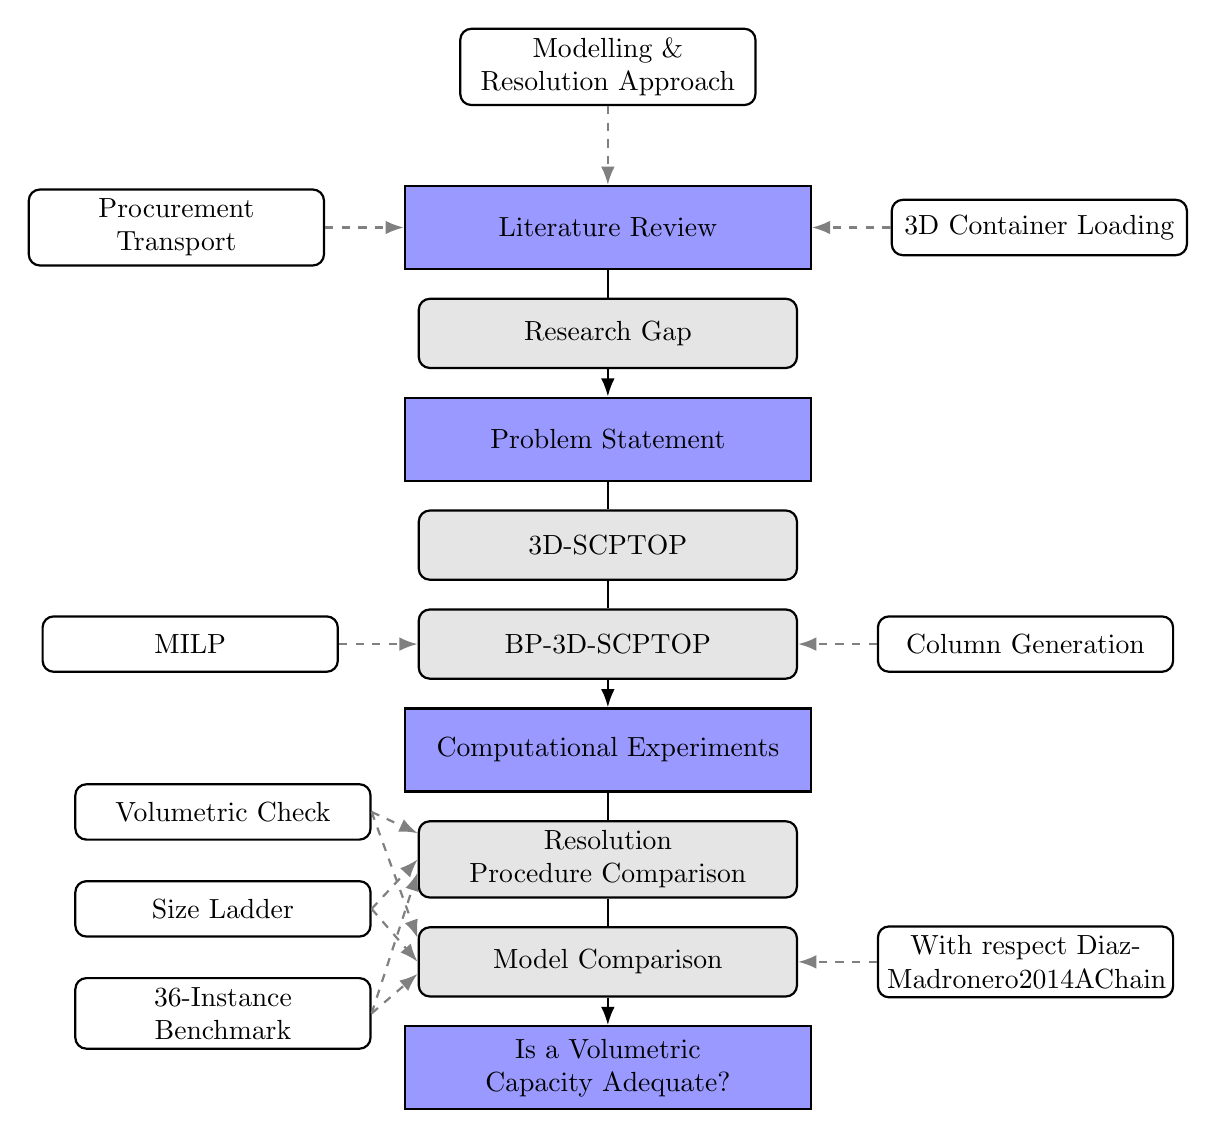
\begin{tikzpicture}[node distance=2cm, auto, thick]

      % Define styles
      \tikzstyle{block} = [rectangle, draw, fill=blue!40, text width=14em, text centered,  minimum height=3em]
      \tikzstyle{sideblock} = [rectangle, draw, fill=white, text width=10em, text centered, rounded corners, minimum height=2em]
      \tikzstyle{grayblock} = [rectangle, draw, fill=gray!20, text width=13em, text centered, rounded corners, minimum height=2.5em]
      \tikzstyle{line} = [draw, -Latex]
      \tikzstyle{plainline} = [draw]
      \tikzstyle{dashedline} = [draw, dashed, gray, thick, -Latex]





      % Central nodes
      \node [block] (literature) {Literature Review};
      \node [grayblock, below=0.35cm of literature] (research) {Research Gap};
      \node [block, below=0.35cm of research] (problem) {Problem Statement};
      \node [grayblock, below=0.35cm of problem] (3dMilp) {3D-SCPTOP};
      \node [grayblock, below=0.35cm of 3dMilp] (3dMH) {BP-3D-SCPTOP};
      \node [block, below=0.35cm of 3dMH] (experiments) {Computational Experiments};
      \node [grayblock, below=0.35cm of experiments] (procedure) {Resolution \\ Procedure Comparison};
      \node [grayblock, below=0.35cm of procedure] (comparison) {Model Comparison};
      \node[ aux_gene_group,fit=(comparison) (procedure)] (gr1) {};

      \node [block, below=0.35cm of comparison] (case) {Is a Volumetric \\ Capacity Adequate?};

      % Side nodes
      \node [sideblock, above=1cm of literature] (model) {Modelling \& \\ Resolution Approach};
      \node [sideblock, left=1cm of literature] (procurement) {Procurement Transport};
      \node [sideblock, right=1cm of literature] (3D) {3D Container Loading};

      % Draw edges for side nodes (with dashed gray lines and arrows)
      \path [dashedline] (3D) -- (literature);
      \path [dashedline] (model) -- (literature);
      \path [dashedline] (procurement) -- (literature);

      % Side nodes
      \node [sideblock, left=1cm of 3dMH] (MILP) {MILP};
      \node [sideblock, right=1cm of 3dMH] (MetaHeuristic) {Column Generation};

      % Draw edges for side nodes (with dashed gray lines and arrows)
      \path [dashedline] (MILP) -- (3dMH);
      \path [dashedline] (MetaHeuristic) -- (3dMH);

      % % Side nodes
      % \node [sideblock, above left=1.25cm and 1cm of comparison] (small) {Small Instances};
      % \node [sideblock, below=0.5cm of small] (medium) {Medium Instances};
      % \node [sideblock, below=0.5cm of medium] (large) {Large Instances};

      % Side nodes
      \node [sideblock, left=0.5cm of gr1] (medium) {Size Ladder};

      \node [sideblock, above=0.5cm of medium] (small) {Volumetric Check};
      \node [sideblock, below=0.5cm of medium] (large) {36-Instance Benchmark};

      \coordinate (center13) at ($(procedure.west)!1/3!(procedure.south west)$);
      \coordinate (center12) at ($(procedure.west)$);
      \coordinate (center23) at ($(procedure.west)!2/3!(procedure.north west)$);


      % Draw edges for side nodes (with dashed gray lines and arrows)
      \path [dashedline] (small.east) -- (center23) ;
      \path [dashedline] (medium.east)  -- (center12) ;
      \path [dashedline](large.east)  -- (center13) ;


      \coordinate (ccenter13) at ($(comparison.west)!1/3!(comparison.south west)$);
      \coordinate (ccenter12) at ($(comparison.west)$);
      \coordinate (ccenter23) at ($(comparison.west)!2/3!(comparison.north west)$);


      % Draw edges for side nodes (with dashed gray lines and arrows)
      \path [dashedline] (small.east) -- (ccenter23) ;
      \path [dashedline] (medium.east)  -- (ccenter12) ;
      \path [dashedline](large.east)  -- (ccenter13) ;




      % Draw edges for central nodes and gray nodes
      \path [plainline] (literature)  -- (research);
      \path [line] (research) -- (problem);
      \path [plainline] (problem)  -- (3dMilp);
      \path [plainline] (3dMilp)  -- (3dMH);
      \path [line] (3dMH) -- (experiments);
      \path [plainline] (experiments)  -- (procedure);
      \path [plainline] (procedure)  -- (comparison);
      \path [line] (comparison) -- (case);






      % Side nodes
      \node [sideblock, right=1cm of comparison] (reference) {With respect \autocite{Diaz-Madronero2014AChain}};

      % Draw edges for side nodes (with dashed gray lines and arrows)
      \path [dashedline] (reference) -- (comparison);







    \end{tikzpicture}
  }
  \caption{Research Methodology}
  \label{fig:tikz1}
\end{figure}

\FloatBarrier

\section{Problem description}
\label{sec:problem}

A plant assembles products supplied by a single supplier over a finite
horizon. Every product travels in exactly one type of RTI: a rigid
container, \emph{erected} while it carries product and \emph{folded}
when empty, so one physical container occupies two different volumes
depending on which way it is moving. The supplier packs its production
into erected RTIs and ships them to the plant; the plant consumes the
product, folds the containers and returns them. Both legs are run with
identical trailers, every dispatch costs the same whatever it carries,
and a trailer may be dispatched only if it is full. A dispatch arrives
after a lead time of $lt\ge1$ periods and is available at neither end
in between, and each node must end every period holding enough stock to
cover the next periods of its own activity. What has to be decided is,
per direction and period, how many trucks go, what each carries and
what consequently sits in stock; the cost is the number of dispatches
plus the inventory held.

Two features separate this from a transport-and-inventory model. The
two flows are coupled through the containers themselves --- the plant
can return only empties it has emptied and the supplier can fill only
containers it has received --- so a shortage on the return leg
propagates into the delivery leg one lead time later. And the
admissibility of a truck load is a three-dimensional packing condition
rather than a capacity inequality: a load whose volume and weight both
fit may still have no arrangement inside the trailer. Loading is
represented through \emph{stacks} of whole homogeneous layers rather
than through the placement of individual RTIs, which makes the stacks
self-supporting, so no vertical-stability constraint is needed.

\section{The 3D-SCPTOP formulation}
\label{sec:model}

The model is written over \emph{trucks}. A dispatched truck designs its
own layout --- the stack types, orientations, positions and layer
compositions of its slots are variables of that truck and that period,
and its load is assigned to those slots in the same period --- so there
is no catalogue of loading configurations. That is the decision
Section~\ref{sec:decomp} rests on: every row below carries either the
triple $(g,k,t)$ or none of it, so the model is block-angular over
$G\times K\times T$ and the pricing problem of the Dantzig--Wolfe
reformulation is obtained by deleting that quantifier and nothing
else.

Throughout, $g\in G=\{s,p\}$ indexes nodes and directions (named by
destination), $n\in N$ products, $r\in R$ RTI types, $h\in H$ stack
types, $i,j\in I$ slot positions, $k\in K$ trucks and $t\in T$ periods,
with $\rho(n)$ the RTI type product $n$ travels in and
$M(r)=\{n:\rho(n)=r\}$; variables whose direction is fixed by
definition omit $g$. Table \ref{tab:sb-Nomenclature} is the
nomenclature.

\begin{longtable}[hbt!]{|p{0.15\textwidth}|p{0.79\textwidth}|}
    \caption{Nomenclature. The pricing problem of
    Section~\ref{sec:pricing} is one block of this model with the index
    $(g,k,t)$ deleted, so it reuses these symbols with that index
    dropped; the three variables it adds are listed last.}
    \label{tab:sb-Nomenclature}\\
    \hline
    \multicolumn{2}{|l|}{\textbf{Indices and sets}}\\\hline
    $G$            & Supplier and plant nodes, $G=\{s,p\}$; $g=s$ is the folded
                     direction (plant to supplier), $g=p$ the full one.\\
    $N$, $R$, $H$  & Products, RTI types, stack types.\\
    $I$            & Stack-slot indices on a truck floor, bounded by
                     \eqref{sb:eq:Ibound}.\\
    $K$, $T$       & Trucks available per direction and period; planning periods.\\
    $\rho(n)$, $M(r)$ & The RTI type product $n$ travels in; the products type $r$
                     carries, $M(r)=\{n:\rho(n)=r\}$.\\
    $R(h)$         & RTI types compatible with stack type $h$.\\
    \hline
    \multicolumn{2}{|l|}{\textbf{Parameters}}\\\hline
    $cK$           & Cost of dispatching one truck.\\
    $lt$, $SC$     & Lead time, $lt\ge1$; coverage window, in periods.\\
    $i_{gn}$, $ie_{gr}$ & Initial inventory at $g$ of full RTIs of $n$, of folded RTIs of $r$.\\
    $ic_{gn}$      & Inventory holding cost of $n$ at $g$.\\
    $d_{gnt}$      & Production plan for $n$ at $g$ in $t$: filled at $s$, consumed at $p$.\\
    $a_{nt}$, $ae_{rt}$ & Pipeline arrivals at $p$, respectively $s$, in $t\le lt$.\\
    $ss_{gnt}$, $sse_{gtr}$ & Coverage stock of full, respectively folded, RTIs
                     \eqref{sb:eq:coverage}.\\
    $w_{n}$, $w^{\mathrm{f}}_{r}$ & Weight of a full RTI carrying $n$; of a folded
                     RTI of type $r$. Both $>0$.\\
    $pK^{w}$, $W^{\max}$ & Truck payload; per-stack crush-limit cap on the
                     \emph{total} weight of one stack, over all its layers.\\
    $pK,qK,rK$     & Truck floor length, floor width, inner height;
                     $\Gamma_{K}=pK\cdot qK\cdot rK$.\\
    $\alpha$       & Minimum truck utilisation, on whichever of volume or payload
                     binds, $0<\alpha\le1$.\\
    $p_{h},q_{h}$  & Footprint length and width of stack type $h$.\\
    $r_{gr}$, $a_{r}$, $\gamma_{gr}$ & Height of one RTI of type $r$ at node $g$
                     (full at $p$, folded at $s$); its footprint area; its volume
                     $\gamma_{gr}=a_{r}r_{gr}$.\\
    $n_{hr}$       & RTIs of type $r\in R(h)$ per layer of stack type $h$; one layer
                     tiles the footprint, $n_{hr}a_{r}=p_{h}q_{h}$.\\
    $\hat w_{gr}$  & Weight per RTI in the layer-capacity form of the utilisation
                     floor: $\hat w_{sr}=w^{\mathrm{f}}_{r}$,
                     $\hat w_{pr}=\max_{n\in M(r)}w_{n}$.\\
    $\eta^{K},\eta^{I}$ & Weights of the transport and inventory objectives;
                     both $1$ throughout.\\
    $M^{x},M^{y}$  & Big-$M$ constants of the non-overlap rows, $M^{x}=pK$, $M^{y}=qK$.\\
    $\bar u^{V}_{n}$, $\bar u^{\mathrm{e}}_{r}$ & $\lfloor W^{\max}/w_{n}\rfloor$ full
                     RTIs of $n$ per slot; $\lfloor pK^{w}/w^{\mathrm{f}}_{r}\rfloor$
                     folded RTIs of $r$ per truck.\\
    \hline
    \multicolumn{2}{|l|}{\textbf{Decision variables --- the truck and its layout}}\\\hline
    $Z_{gkt}$        & $\in\{0,1\}$. Truck $k$ of direction $g$ in $t$ is configured,
                       i.e.\ carries a layout.\\
    $Y_{gkt}$        & $\in\{0,1\}$. That truck is dispatched.\\
    $\theta_{gkt}$   & $\in\{0,1\}$. Selects the resource on which its utilisation
                       floor is required: volume if $1$, payload if $0$.\\
    $X_{gihkt}$      & $\in\{0,1\}$. Slot $i$ holds a stack of type $h$.\\
    $L_{gihktr}$     & $\in\mathbb{Z}_{\ge 0}$. Layers of RTI type $r\in R(h)$ in slot $i$.\\
    $LX_{gihkt},LY_{gihkt}$ & $\in\{0,1\}$. Stack $h$'s length lies along the $x$-,
                       respectively $y$-axis in slot $i$.\\
    $PX_{gikt},PY_{gikt}$ & $\ge 0$. Bottom-left coordinates of slot $i$ on the floor.\\
    $A,B,C,D$ (on $gijkt$) & $\in\{0,1\}$. Which of the four separating
                       half-planes resolves the overlap of slots $i$ and $j$.\\
    \hline
    \multicolumn{2}{|l|}{\textbf{Decision variables --- load and inventory}}\\\hline
    $V_{kint}$       & $\in\mathbb{Z}_{\ge 0}$. Full RTIs of $n$ in slot $i$ of
                       plant-bound truck $k$ in $t$.\\
    $V^{\mathrm{e}}_{krt}$ & $\in\mathbb{Z}_{\ge 0}$. Folded RTIs of type $r$ on
                       supplier-bound truck $k$ in $t$.\\
    $I_{gnt}$, $Ie_{gtr}$ & $\in\mathbb{Z}_{\ge 0}$. End-of-period inventory of full
                       RTIs of $n$, of folded RTIs of $r$, at $g$.\\
    \hline
    \multicolumn{2}{|l|}{\textbf{Derived quantities} (abbreviations, \eqref{sb:eq:agg-V}--\eqref{sb:eq:agg-L})}\\\hline
    $\overline{V}_{nt}$, $\overline{V^{\mathrm{e}}}_{rt}$ & Full RTIs of $n$ delivered
                       to the plant in $t$; folded RTIs of $r$ returned to the supplier.\\
    $\overline{V}_{knt}$ & Full RTIs of $n$ on plant-bound truck $k$ in $t$.\\
    $\widehat{X}_{gikt}$, $\overline{L}_{ghktr}$ & Slot $i$ is used; layers of type $r$
                       under stack type $h$ on that truck, over all slots.\\
    \hline
    \multicolumn{2}{|l|}{\textbf{Added by the reformulation} (Sections \ref{sec:master}--\ref{sec:pricing})}\\\hline
    $\lambda^{g}_{\omega t}$ & $\in\mathbb{Z}_{\ge0}$. Trucks of class $(g,t)$
                       dispatched carrying column $\omega$.\\
    $\pi_{nt},\pi_{rt}$, $\mu_{gt}$ & Duals of \eqref{bp:MP-def-V}--\eqref{bp:MP-def-Ve},
                       respectively of \eqref{bp:MP-count} and of every further row a
                       dispatch variable of $(g,t)$ occupies.\\
    $n_{gt}$, $X$    & Dispatch total of class $(g,t)$, $n_{gt}=\sum_{\omega}
                       \lambda^{g}_{\omega t}$; the fleet $X=\sum_{g,t}n_{gt}$.\\
    \hline
\end{longtable}


\subsection{Derived quantities}

Five sums recur, as \emph{abbreviations} and not constraints.
\begin{align}
\overline{V}_{nt}&=\sum_{k\in K}\sum_{i\in I} V_{kint}
    &&\forall n\in N,\; t\in T
    \label{sb:eq:agg-V}\\
\overline{V^{\mathrm{e}}}_{rt}&=\sum_{k\in K} V^{\mathrm{e}}_{krt}
    &&\forall r\in R,\; t\in T
    \label{sb:eq:agg-Ve}\\
\overline{V}_{knt}&=\sum_{i\in I} V_{kint}
    &&\forall k\in K,\; n\in N,\; t\in T
    \label{sb:eq:agg-Vk}\\
\widehat{X}_{gikt}&=\sum_{h\in H} X_{gihkt}
    &&\forall g\in G,\; i\in I,\; k\in K,\; t\in T
    \label{sb:eq:agg-X}\\
\overline{L}_{ghktr}&=\sum_{i\in I} L_{gihktr}
    &&\forall g\in G,\; h\in H,\; k\in K,\; t\in T,\; r\in R(h)
    \label{sb:eq:agg-L}
\end{align}
The first two carry the method. The inventory block reads
$\overline{V}_{nt}$ and $\overline{V^{\mathrm{e}}}_{rt}$ and nothing
else about the trucks --- not which truck carried what, nor how the
load was placed.

\subsection{Objective}

Transport cost counts \emph{dispatches}, so a configured but
undispatched truck costs nothing; holding cost falls on erected RTIs.
\begin{align}
\min\; z^{K} &= \sum_{g\in G}\sum_{k\in K}\sum_{t\in T} cK\cdot Y_{gkt},
\qquad
\min\; z^{I} = \sum_{g\in G}\sum_{n\in N}\sum_{t\in T} ic_{gn}\cdot I_{gnt}
    \label{sb:eq:obj-zK}\\
\min\;& \eta^{K} z^{K}+\eta^{I} z^{I},
    \qquad \eta^{K}=\eta^{I}=1 \text{ throughout},
\label{sb:eq:obj}
\end{align}
\subsection{Inventory, flow balance and coverage}

Arrivals are delayed; inventory itself accumulates one period at a
time. For the plant,
\begin{align}
I_{pnt}  &=I_{p,n,t-1}-d_{pnt}+\overline{V}_{n,t-lt}
    &&\forall n\in N,\; t\ge lt+1
    \label{sb:eq:inv-plant-main}\\
I_{pnt}  &=I_{p,n,t-1}-d_{pnt}+a_{nt}
    &&\forall n\in N,\; t\in\{2,\dots,lt\}
    \label{sb:eq:inv-plant-transient}\\
I_{pnt}  &=i_{pn}-d_{pnt}+a_{nt}
    &&\forall n\in N,\; t=1
    \label{sb:eq:inv-plant-init}\\
Ie_{ptr} &=Ie_{p,t-1,r}+\sum_{n\in M(r)} d_{pnt}-\overline{V^{\mathrm{e}}}_{rt}
    &&\forall r\in R,\; t\ge 2
    \label{sb:eq:inve-plant}\\
Ie_{ptr} &=ie_{pr}+\sum_{n\in M(r)} d_{pnt}-\overline{V^{\mathrm{e}}}_{rt}
    &&\forall r\in R,\; t=1
    \label{sb:eq:inve-plant-init}
\end{align}
Consuming a full RTI produces a folded one in the same period, which is
why $d_{pnt}$ drives \eqref{sb:eq:inve-plant}. For the supplier,
\begin{align}
I_{snt}  &=I_{s,n,t-1}+d_{snt}-\overline{V}_{nt}
    &&\forall n\in N,\; t\ge 2
    \label{sb:eq:inv-sup-main}\\
I_{snt}  &=i_{sn}+d_{snt}-\overline{V}_{nt}
    &&\forall n\in N,\; t=1
    \label{sb:eq:inv-sup-init}\\
Ie_{str} &=Ie_{s,t-1,r}+\overline{V^{\mathrm{e}}}_{r,t-lt}-\sum_{n\in M(r)} d_{snt}
    &&\forall r\in R,\; t\ge lt+1
    \label{sb:eq:inve-sup-main}\\
Ie_{str} &=Ie_{s,t-1,r}+ae_{rt}-\sum_{n\in M(r)} d_{snt}
    &&\forall r\in R,\; t\in\{2,\dots,lt\}
    \label{sb:eq:inve-sup-transient}\\
Ie_{str} &=ie_{sr}+ae_{rt}-\sum_{n\in M(r)} d_{snt}
    &&\forall r\in R,\; t=1
    \label{sb:eq:inve-sup-init}
\end{align}
The lead time therefore acts on one side of a balance only --- the
sending node's stock falls in the dispatch period, the receiving node's
rises $lt$ periods later --- an alignment
Section~\ref{sec:branching} uses twice. Coverage stock is enforced at
both nodes and on both kinds of stock,
\begin{align}
I_{gnt}\ \ge\ ss_{gnt}
    &&\forall g\in G,\; n\in N,\; t\in T
    \label{sb:eq:safety-full}\\
Ie_{gtr}\ \ge\ sse_{gtr}
    &&\forall g\in G,\; r\in R,\; t\in T
    \label{sb:eq:safety-empty}
\end{align}
the requirement being that node's own series over the next $SC$
periods:
\begin{equation}
ss_{gnt}=\sum_{j=1}^{SC} d_{g,n,\tau(t,j)},
\qquad
sse_{gtr}=\sum_{n\in M(r)} ss_{gnt},
\qquad
\tau(t,j)=\begin{cases} t+j, & t+j\le |T|,\\ |T|-SC+j, & \text{otherwise.}\end{cases}
\label{sb:eq:coverage}
\end{equation}
Near the end of the horizon \eqref{sb:eq:coverage} wraps the window
back onto the last $SC$ periods rather than truncating it, following
\autocite{Diaz-Madronero2014APlanning}: truncating lowers the
requirement of the final periods and with it the optimal value, so the
tail rule belongs to the problem statement.

\subsection{The layout of a truck}

Everything from here to \eqref{sb:eq:stack-w-sup} is written for one
truck: one direction $g$, one index $k$, one period $t$. At most one
stack type occupies a slot and only a configured truck has slots; a
stack is oriented along one axis or the other; its height cannot exceed
the trailer's, which with $r_{gr}>0$ also empties an unused slot:
\begin{align}
  & \widehat{X}_{gikt}\;\le\;Z_{gkt} && \forall i\in I
    \label{sb:eq:slot-active}\\
  & LX_{gihkt}+LY_{gihkt}\;=\;X_{gihkt} && \forall h\in H,\; i\in I
    \label{sb:eq:orient}\\
  & \sum_{r\in R(h)} r_{gr}\,L_{gihktr}\;\le\;rK\cdot X_{gihkt}
    && \forall h\in H,\; i\in I
    \label{sb:eq:height}
\end{align}
Slots must not overlap --- for each pair $i<j$, the usual four-way
disjunction closed by a cover row --- and every slot lies inside the
floor:
\begin{align}
PX_{gikt}+\sum_{h\in H}\bigl(p_{h}LX_{gihkt}+q_{h}LY_{gihkt}\bigr)
    &\le PX_{gjkt}+M^{x}(1-A_{gijkt})
    \label{sb:eq:nonov-x1}\\
PX_{gjkt}+\sum_{h\in H}\bigl(p_{h}LX_{gjhkt}+q_{h}LY_{gjhkt}\bigr)
    &\le PX_{gikt}+M^{x}(1-B_{gijkt})
    \label{sb:eq:nonov-x2}\\
PY_{gikt}+\sum_{h\in H}\bigl(q_{h}LX_{gihkt}+p_{h}LY_{gihkt}\bigr)
    &\le PY_{gjkt}+M^{y}(1-C_{gijkt})
    \label{sb:eq:nonov-y1}\\
PY_{gjkt}+\sum_{h\in H}\bigl(q_{h}LX_{gjhkt}+p_{h}LY_{gjhkt}\bigr)
    &\le PY_{gikt}+M^{y}(1-D_{gijkt})
    \label{sb:eq:nonov-y2}\\
A_{gijkt}+B_{gijkt}+C_{gijkt}+D_{gijkt}
    &\;\ge\;\widehat{X}_{gikt}+\widehat{X}_{gjkt}-1
    \label{sb:eq:cover}\\
PX_{gikt}+\sum_{h\in H}\bigl(p_{h}LX_{gihkt}+q_{h}LY_{gihkt}\bigr)
    &\le pK
    \label{sb:eq:cont-x}\\
PY_{gikt}+\sum_{h\in H}\bigl(q_{h}LX_{gihkt}+p_{h}LY_{gihkt}\bigr)
    &\le qK
    \label{sb:eq:cont-y}
\end{align}
The containment rows are unconditional, which is what lets the
non-overlap rows take the tightened $M^{x}=pK$, $M^{y}=qK$.

\subsection{Full truckload on every dispatched truck}

A dispatched truck must be full, and it can be full in two ways: it may
run out of space or of payload. A volume-only floor is not a
conservative simplification but an infeasible one --- filling the
fraction $\alpha=0.55$ of a $97.92$~m$^{3}$ trailer
($13\,600\times2\,400\times3\,000$~mm) with freight at $579$~kg/m$^{3}$
weighs $31.2$~t against a $24$~t cap, and seven of the industrial
catalogue's fifteen types are denser still. Summing the two ratios is
the opposite error: it accepts a truck $35\%$ full by volume and $20\%$
by weight. We therefore require a fraction $\alpha$ of \emph{either}
resource, a binary $\theta_{gkt}$ selecting which one binds, on the
load the truck carries with each commodity's own weight:
\begin{align}
\sum_{n\in N}\gamma_{p\rho(n)}\,\overline{V}_{knt}
&\;\ge\;\alpha\,\Gamma_{K}\bigl(Y_{pkt}-1+\theta_{pkt}\bigr)
    &&\forall k\in K,\; t\in T
    \label{sb:eq:util-p}\\
\sum_{n\in N} w_{n}\,\overline{V}_{knt}
&\;\ge\;\alpha\,pK^{w}\bigl(Y_{pkt}-\theta_{pkt}\bigr)
    &&\forall k\in K,\; t\in T
    \label{sb:eq:utilw-p}\\
\sum_{r\in R}\gamma_{sr}\,V^{\mathrm{e}}_{krt}
&\;\ge\;\alpha\,\Gamma_{K}\bigl(Y_{skt}-1+\theta_{skt}\bigr)
    &&\forall k\in K,\; t\in T
    \label{sb:eq:util-s}\\
\sum_{r\in R} w^{\mathrm{f}}_{r}\,V^{\mathrm{e}}_{krt}
&\;\ge\;\alpha\,pK^{w}\bigl(Y_{skt}-\theta_{skt}\bigr)
    &&\forall k\in K,\; t\in T
    \label{sb:eq:utilw-s}
\end{align}
Exactly one of each pair is active at $Y_{gkt}=1$, so each is the
disjunction ``full by volume \emph{or} full by payload''. The same
disjunction on the layer \emph{capacity} the stacks provide rather than
on the load they receive,
\begin{align}
  \sum_{h\in H}\sum_{r\in R(h)}
    \gamma_{gr}\,n_{hr}\,\overline{L}_{ghktr}
&\;\ge\;\alpha\,\Gamma_{K}\bigl(Y_{gkt}-1+\theta_{gkt}\bigr),
\quad
  \sum_{h\in H}\sum_{r\in R(h)}
    \hat w_{gr}\,n_{hr}\,\overline{L}_{ghktr}
\;\ge\;\alpha\,pK^{w}\bigl(Y_{gkt}-\theta_{gkt}\bigr)
    \label{sb:eq:util-cap}
\end{align}
is a valid tightening, kept because it lets a solver establish a layout
before choosing a product assignment. Which form is the
\emph{requirement} matters.
\eqref{sb:eq:util-p}--\eqref{sb:eq:utilw-s} is, full truckload being a
property of the freight that moves; \eqref{sb:eq:util-cap} follows from
it because a slot never receives more RTIs of type $r$ than its layers
hold and $\hat w_{gr}\ge w_{n}$ for every $n\in M(r)$, and taken
\emph{alone} would admit trucks that are not full. That inequality is
also why $\hat w_{pr}=\max_{n\in M(r)}w_{n}$ is the family
\emph{maximum}: the family \emph{minimum} would assert that
\emph{every} product assignment of this layout fills the truck, cutting
off feasible loads.

\subsection{Dispatch, loading and weight}

A dispatched truck must be configured,
\begin{equation}
Y_{gkt}\;\le\;Z_{gkt}\qquad\forall g\in G,\;k\in K,\;t\in T,
\label{sb:eq:lc-active}
\end{equation}
while the converse fails: $Z_{gkt}=1$ with $Y_{gkt}=0$ is a truck
carrying a layout and no freight, which in the reformulated block is
exactly the empty column (Section~\ref{sec:pricing}).

Full RTIs in a slot cannot exceed the layer capacity of the stack
placed there, products sharing an RTI type partitioning it; folded RTIs
are capped by the truck's aggregate capacity, folded weight being
deterministic in the type. Both loads are gated on the dispatch, at
their own analytic bounds rather than a generic big-$M$:
\begin{align}
  & \sum_{n\in M(r)} V_{kint}
      \;\le\;\sum_{h\,:\,r\in R(h)} n_{hr}\,L_{p,i,h,k,t,r}
    && \forall k\in K,\; i\in I,\; r\in R,\; t\in T
    \label{sb:eq:slot-cap}\\
  & V^{\mathrm{e}}_{krt}
      \;\le\;\sum_{h\,:\,r\in R(h)} n_{hr}\,\overline{L}_{s,h,k,t,r}
    && \forall k\in K,\; r\in R,\; t\in T
    \label{sb:eq:empty-cap}\\
  & V_{kint}\le \bar u^{V}_{n}\,Y_{pkt}
    && \forall k\in K,\; i\in I,\; n\in N,\; t\in T
    \label{fix:slot-link}\\
  & V^{\mathrm{e}}_{krt}\le \bar u^{\mathrm{e}}_{r}\,Y_{skt}
    && \forall k\in K,\; r\in R,\; t\in T
    \label{fix:empty-link}
\end{align}
The payload is a property of the truck, the crush limit of each stack;
on plant-bound trucks that cap is \emph{period-exact}, evaluated on the
mix actually loaded in the slot, on supplier-bound trucks deterministic
in the layout:
\begin{align}
  & \sum_{n\in N} w_{n}\,\overline{V}_{knt}\;\le\;pK^{w}\,Y_{pkt},
  \qquad
    \sum_{r\in R} w^{\mathrm{f}}_{r}\,V^{\mathrm{e}}_{krt}
      \;\le\;pK^{w}\,Y_{skt}
    && \forall k\in K,\; t\in T
    \label{sb:eq:truck-w-plant}\\
  & \sum_{n\in N} w_{n}\,V_{kint}\;\le\;W^{\max}
    && \forall k\in K,\; i\in I,\; t\in T
    \label{sb:eq:stack-w-plant}\\
  & \sum_{h\in H}\sum_{r\in R(h)}
      w^{\mathrm{f}}_{r}\,n_{hr}\,L_{s,i,h,k,t,r}\;\le\;W^{\max}
    && \forall i\in I,\; k\in K,\; t\in T
    \label{sb:eq:stack-w-sup}
\end{align}
where \eqref{sb:eq:truck-w-plant} names both payload rows and
\eqref{fix:slot-link} is tighter in the relaxation than their
implication, since what bounds a slot's content is the crush cap.

\subsection{Symmetry, slot-set sizing and data assumptions}
\label{sb:sec:symm}

The slots of a truck are interchangeable, and so are the trucks of a
direction and period. Both are ordered:
\begin{align}
  & \widehat{X}_{g,i+1,k,t}\;\le\;\widehat{X}_{gikt}
    && \forall g\in G,\; k\in K,\; t\in T,\; i<|I|
    \label{sb:eq:sym}\\
  & Y_{g,k+1,t}\;\le\;Y_{gkt}
    && \forall g\in G,\; t\in T,\; k<|K|
    \label{dec:sym-truck}
\end{align}
Re-indexing makes \eqref{dec:sym-truck} valid, but it removes only
\emph{which} subset of trucks is used: loads and layouts stay
interchangeable among those used, so a plan dispatching $m$ trucks in a
period still appears $m!$ times --- the difficulty
Section~\ref{sec:decomp} removes by aggregation rather than by a row.
The slot count is a modelling parameter, and
\begin{equation}
|I|\;\le\;\Bigl\lfloor
    (pK\cdot qK)\big/\min_{h\in H} p_{h}q_{h}
\Bigr\rfloor
\label{sb:eq:Ibound}
\end{equation}
eliminates provably unused slot variables without cutting any feasible
layout. It is more than preprocessing: a placement model given fewer
slots than a layout needs can report infeasible while the load is
placeable (Section~\ref{sec:pricing}).

Four properties of the data are assumed: $\rho$ is a partition;
$lt\ge1$, which the lagged terms require; all weights and heights are
strictly positive, which makes $\bar u^{V}_{n}$ and
$\bar u^{\mathrm{e}}_{r}$ well defined and lets \eqref{sb:eq:height}
empty an unused slot; and the footprint geometry is consistent, one
layer of stack type $h$ tiling its footprint, $n_{hr}a_{r}=p_{h}q_{h}$,
with the volume charged to an RTI its bounding box,
$\gamma_{gr}=a_{r}r_{gr}$. \emph{The last is a departure}, and
Proposition~\ref{prop:inclusion} and the floor-area inequality
\eqref{bp:PP-areacut} are both false without it. It costs nothing
here, both instance families building one stack type per distinct RTI
footprint, so $n_{hr}=1$ and the relation is an identity.

\subsection{Domains}

\begin{align*}
&Z_{gkt},\,Y_{gkt},\,\theta_{gkt},\,X_{gihkt},\,LX_{gihkt},\,LY_{gihkt},\,
  A_{gijkt},\,B_{gijkt},\,C_{gijkt},\,D_{gijkt}\in\{0,1\},\\
&L_{gihktr},\,V_{kint},\,V^{\mathrm{e}}_{krt},\,I_{gnt},\,Ie_{gtr}
  \in\mathbb{Z}_{\ge 0},\qquad
PX_{gikt},\,PY_{gikt}\ge 0.
\end{align*}

\section{Decomposition and master problem}
\label{sec:decomp}

3D-SCPTOP carries a complete two-dimensional packing problem for every
truck of every direction and period --- $2|K||T|$ replicas, each with
$4\binom{|I|}{2}$ big-$M$ disjunctions
\eqref{sb:eq:nonov-x1}--\eqref{sb:eq:nonov-y2} whose linear relaxation
is weak --- and the replicas are interchangeable, so every solution
appears a factorial number of times. Both difficulties disappear when
the unit of decision is a complete loaded truck: the geometry moves into
one pricing problem per direction, and identical trucks are counted
rather than indexed. The Dantzig--Wolfe reformulation below
\autocite{DantzigWolfe1960,Barnhart1998BranchAndPrice,Desaulniers2005ColumnGeneration}
does both without restricting anything (Figure~\ref{fig:blocks};
Table~\ref{tab:rowmap} in Appendix~\ref{appendix:rowmap} maps the rows).

% F1 of article/paper-figures.md: the block-angular constraint matrix of the
% compact model, and the structural move the derivation rests on.  Greys only,
% so it survives a greyscale print; the braces need decorations.pathreplacing,
% loaded in paper.tex.
\providecommand{\blknohyph}{\hyphenpenalty=10000\exhyphenpenalty=10000\relax}
\begin{figure}[!t]
\centering
\resizebox{\textwidth}{!}{%
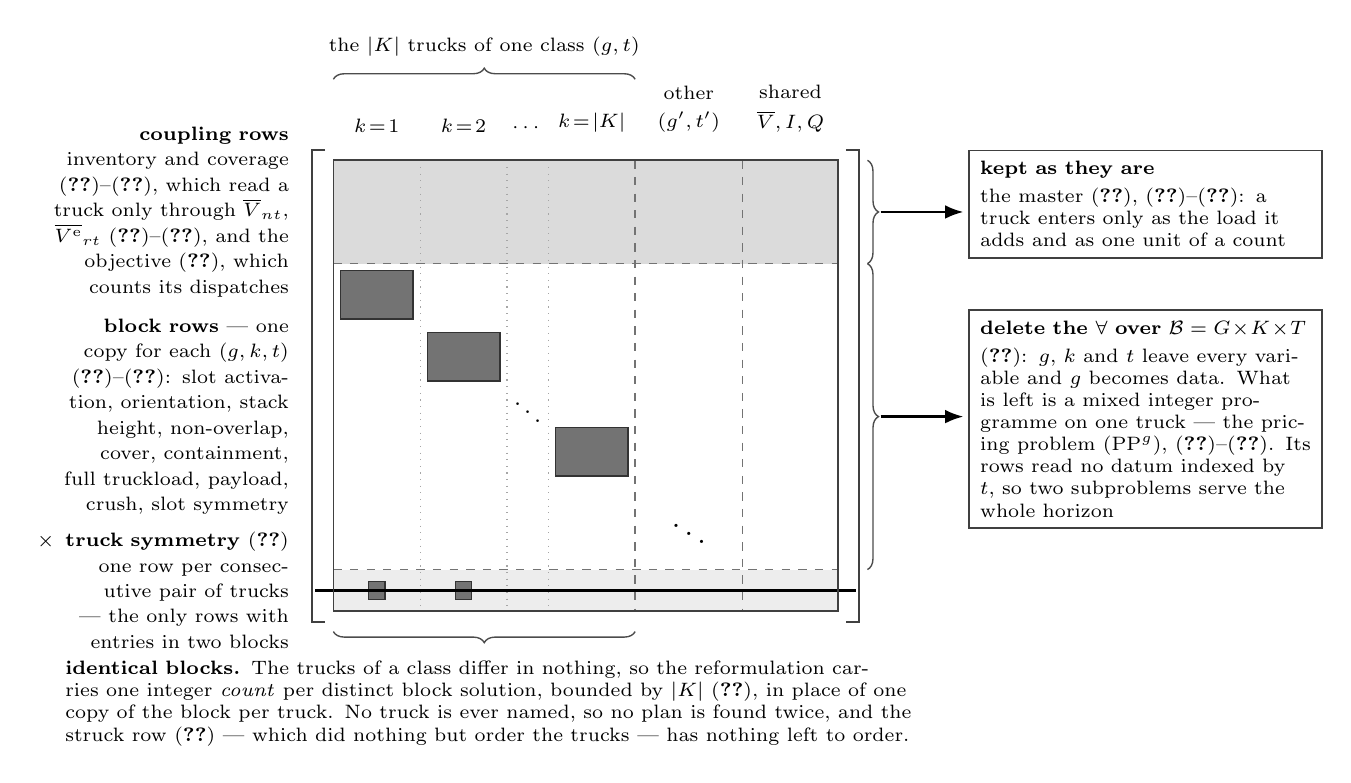
\begin{tikzpicture}[>=Latex, x=1.05cm, y=1.05cm,
  cpl/.style={fill=black!14, draw=none},
  blk/.style={fill=black!55, draw=black!80, line width=0.5pt},
  sep/.style={draw=black!35, dotted, line width=0.4pt},
  cls/.style={draw=black!55, dashed, line width=0.5pt},
  brc/.style={decorate, black!70, line width=0.5pt},
  box/.style={draw=black!75, fill=white, line width=0.6pt, inner sep=4pt,
              align=left, font=\scriptsize, text width=42mm,
              execute at begin node=\blknohyph},
  rl/.style={font=\scriptsize\linespread{1.15}\selectfont, align=right,
             text width=32mm, anchor=east, execute at begin node=\blknohyph},
  hd/.style={font=\scriptsize, align=center, anchor=south},
  nt/.style={font=\scriptsize, align=left, execute at begin node=\blknohyph}]

  % ---- column boundaries (x) and row boundaries (y) ---------------------
  \def\xa{0}    \def\xb{1.05} \def\xc{2.10} \def\xd{2.60}
  \def\xe{3.65} \def\xf{4.95} \def\xg{6.10}
  \def\ya{0}    \def\yb{-1.25}
  \def\yc{-2.00}\def\yd{-2.75}\def\ye{-3.15}\def\yf{-3.90}\def\yg{-4.95}
  \def\yh{-5.45}

  % ---- the coupling band, with entries in every column ------------------
  \fill[cpl] (\xa,\ya) rectangle (\xg,\yb);

  % ---- the diagonal: one block per (g,k,t), nothing off it --------------
  \fill[blk] (0.085,-1.33) rectangle (0.965,-1.92);
  \fill[blk] (1.135,-2.08) rectangle (2.015,-2.67);
  \fill[blk] (2.685,-3.23) rectangle (3.565,-3.82);
  \node[font=\small] at (2.35,-2.95) {$\ddots$};
  \node[font=\large] at (4.30,-4.42) {$\ddots$};

  % ---- the one row that is not block-diagonal, struck out ---------------
  \fill[black!7]  (\xa,\yg)    rectangle (\xg,\yh);
  \fill[black!55, draw=black!80, line width=0.4pt]
     (0.425,-5.09) rectangle (0.625,-5.31);
  \fill[black!55, draw=black!80, line width=0.4pt]
     (1.475,-5.09) rectangle (1.675,-5.31);
  \draw[black, line width=1.1pt] (-0.22,-5.20) -- (6.32,-5.20);

  % ---- grid: column groups, and the two row bands -----------------------
  \foreach \x in {\xb,\xc,\xd} \draw[sep] (\x,\ya) -- (\x,\yh);
  \draw[cls] (\xe,\ya) -- (\xe,\yh);
  \draw[cls] (\xf,\ya) -- (\xf,\yh);
  \draw[cls] (\xa,\yb) -- (\xg,\yb);
  \draw[cls] (\xa,\yg) -- (\xg,\yg);
  \draw[black!75, line width=0.6pt] (\xa,\ya) rectangle (\xg,\yh);
  \draw[black!75, line width=0.7pt]
     (-0.10,0.13) -- (-0.26,0.13) -- (-0.26,-5.58) -- (-0.10,-5.58);
  \draw[black!75, line width=0.7pt]
     (6.20,0.13) -- (6.36,0.13) -- (6.36,-5.58) -- (6.20,-5.58);

  % ---- column headers ---------------------------------------------------
  \node[hd] at (0.525,0.22) {$k\!=\!1$};
  \node[hd] at (1.575,0.22) {$k\!=\!2$};
  \node[hd] at (2.350,0.22) {$\cdots$};
  \node[hd] at (3.125,0.22) {$k\!=\!|K|$};
  \node[hd, text width=13mm] at (4.30,0.22) {other\\[2pt]$(g',t')$};
  \node[hd, text width=12mm] at (5.53,0.22) {shared\\[3pt]$\overline{V},I,Q$};
  \draw[brc, decoration={brace, amplitude=4pt}] (\xa,0.98) -- (\xe,0.98);
  \node[font=\scriptsize, anchor=south] at (1.825,1.14)
     {the $|K|$ trucks of one class $(g,t)$};

  % ---- row labels -------------------------------------------------------
  \node[rl] at (-0.42,-0.625)
     {\textbf{coupling rows}\\ inventory and coverage
      \eqref{sb:eq:inv-plant-main}--\eqref{sb:eq:safety-empty}, which read a
      truck only through $\overline{V}_{nt}$, $\overline{V^{\mathrm{e}}}_{rt}$
      \eqref{sb:eq:agg-V}--\eqref{sb:eq:agg-Ve}, and the objective
      \eqref{sb:eq:obj}, which counts its dispatches};
  \node[rl] at (-0.42,-3.10)
     {\textbf{block rows} --- one copy for each $(g,k,t)$\\
      \eqref{sb:eq:slot-active}--\eqref{sb:eq:sym}: slot activation,
      orientation, stack height, non-overlap, cover, containment,
      full truckload, payload, crush, slot symmetry};
  \node[rl] at (-0.42,-5.20)
     {$\times$\, \textbf{truck symmetry} \eqref{dec:sym-truck}\\
      one row per consecutive pair of trucks --- the only rows with entries
      in two blocks};

  % ---- what each band becomes ------------------------------------------
  \draw[brc, decoration={brace, mirror, amplitude=4pt}] (6.46,\yb) -- (6.46,\ya);
  \draw[->, line width=0.8pt] (6.62,-0.625) -- (7.62,-0.625);
  \node[box, anchor=north west] at (7.68,0.13)
     {\textbf{kept as they are}\\[2pt]
      the master \eqref{eq:MPObjective},
      \eqref{bp:MP-def-V}--\eqref{bp:MP-count}: a truck enters only as the
      load it adds and as one unit of a count};

  \draw[brc, decoration={brace, mirror, amplitude=4pt}] (6.46,\yg) -- (6.46,\yb);
  \draw[->, line width=0.8pt] (6.62,-3.10) -- (7.62,-3.10);
  \node[box, anchor=north west] at (7.68,-1.80)
     {\textbf{delete the $\forall$ over
      $\mathcal{B}=G\!\times\!K\!\times\!T$}\\[2pt]
      \eqref{eq:deletequant}: $g$, $k$ and $t$ leave every variable and $g$
      becomes data. What is left
      is a mixed integer programme on one truck --- the pricing problem
      $(\mathrm{PP}^{g})$, \eqref{bp:PP-objective}--\eqref{bp:PP-utilw}. Its
      rows read no datum indexed by $t$, so two subproblems serve the whole
      horizon};

  % ---- the aggregation, under the diagonal ------------------------------
  \draw[brc, decoration={brace, mirror, amplitude=4pt}] (\xa,-5.70) -- (\xe,-5.70);
  \node[nt, anchor=north, text width=108mm] at (1.90,-5.94)
     {\textbf{identical blocks.} The trucks of a class differ in nothing, so
      the reformulation carries one integer \emph{count} per distinct block
      solution, bounded by $|K|$ \eqref{bp:MP-count}, in place of one copy of
      the block per truck. No truck is ever named, so no plan is found twice,
      and the struck row \eqref{dec:sym-truck} --- which did nothing but order
      the trucks --- has nothing left to order.};

\end{tikzpicture}}
\caption{The decomposition read off the formulation. Every geometric,
stacking, crush, payload and full-truckload row of
Section~\ref{sec:model} is confined to one truck, so the matrix is
block-angular over $\mathcal{B}=G\times K\times T$; deleting the
quantifier over $\mathcal{B}$ from those rows leaves the pricing
problem, and no geometry stays behind in the master.}
\label{fig:blocks}
\end{figure}


Every row from \eqref{sb:eq:slot-active} to \eqref{dec:sym-truck}
carries a single direction, truck and period, and none couples two of
them except \eqref{dec:sym-truck}, which relates truck $k+1$ to truck
$k$; the inventory and coverage rows
\eqref{sb:eq:inv-plant-main}--\eqref{sb:eq:safety-empty} see the
trucks only through the aggregates
\eqref{sb:eq:agg-V}--\eqref{sb:eq:agg-Ve} and the dispatch count. The
formulation is therefore block-angular over $\mathcal{B}=G\times
K\times T$, and removing the quantifier over $\mathcal{B}$ from the
block rows leaves a mixed integer programme over one truck, the pricing
problem $(\mathrm{PP}^{g})$ of Section~\ref{sec:pricing}; for the
stack-height row,
\begin{equation}
\underbrace{\sum_{r\in R(h)} r_{gr}L_{gihktr}\le rK\,X_{gihkt}
  \quad\forall g,h,i,k,t}_{\text{3D-SCPTOP, }\eqref{sb:eq:height}}
\;\longmapsto\;
\underbrace{\sum_{r\in R(h)} r_{gr}L_{ihr}\le rK\,X_{ih}
  \quad\forall h,i}_{(\mathrm{PP}^{g}),\ \eqref{bp:PP-height}},
\label{eq:deletequant}
\end{equation}
The trucks of a class $(g,t)$ are anonymous, so their blocks are
aggregated into one integer variable per block solution, counting the
trucks that take it and bounded by $|K|$; the order of the trucks, and
with it \eqref{dec:sym-truck}, disappears, and the two binaries of
\eqref{sb:eq:lc-active} collapse into one (Section~\ref{sec:pricing}).
The pricing rows read no datum indexed by $t$, so one pricing problem
per direction serves every period, the periods differing only in their
duals. Every block variable that reaches the master is integer, so a
column may be taken to be an integer point of its pricing problem
completed by placement coordinates.

\subsection{Columns}
\label{sec:columns}

A column of a direction is the image of a feasible point of that
direction's pricing problem, kept together with the point as a witness;
$\Omega^{p}$ and $\Omega^{s}$ are the two column sets, indexed by
$\omega$. A \emph{plant-bound} column $\omega\in\Omega^{p}$ is a vector
$b_{\omega}=(b_{\omega n})_{n\in N}$ of full RTIs for which there exist
a slot count $m\le|I|$, stack types $h_{1},\dots,h_{m}\in H$,
orientations, bottom-left coordinates $(x_{i},y_{i})$, layer counts
$\ell_{ir}$ and per-slot product loads $v_{in}$ such that
\begin{align}
&\text{the $m$ footprints, rotated as chosen, do not overlap and lie
   inside } pK\times qK,
   \label{eq:col-geom}\\
&\textstyle\sum_{r\in R(h_{i})} r_{pr}\ell_{ir}\;\le\;rK
   &&\forall i\le m,
   \label{eq:col-height}\\
&\textstyle\sum_{n\in M(r)} v_{in}\;\le\;n_{h_{i}r}\ell_{ir}
   &&\forall i\le m,\;r\in R,
   \label{eq:col-assign}\\
&\textstyle\sum_{n\in N} w_{n}v_{in}\;\le\;W^{\max}
   &&\forall i\le m,
   \label{eq:col-crush}\\
&\textstyle\sum_{n\in N} w_{n}b_{\omega n}\;\le\;pK^{w},
   \qquad
   \max\Bigl\{\tfrac{\sum_{n}\gamma_{p\rho(n)}b_{\omega n}}{\Gamma_{K}},\;
              \tfrac{\sum_{n}w_{n}b_{\omega n}}{pK^{w}}\Bigr\}\;\ge\;\alpha,
   \label{eq:col-truck}\\
&b_{\omega n}=\textstyle\sum_{i\le m} v_{in}
   &&\forall n\in N.
   \label{eq:col-agg}
\end{align}
These are the block rows of Section~\ref{sec:model} read on one truck;
in \eqref{eq:col-assign} $n_{h_{i}r}\ell_{ir}$ is read as $0$ for
$r\notin R(h_{i})$, and a partly filled layer is a legal layout. A
\emph{supplier-bound} column $e_{\omega}=(e_{\omega r})_{r\in R}$ is
the analogous object over folded RTIs, with \eqref{sb:eq:stack-w-sup}
as its crush condition and
$e_{\omega r}\le\sum_{i\le m}n_{h_{i}r}\ell_{ir}$
\eqref{sb:eq:empty-cap} in place of \eqref{eq:col-assign} and
\eqref{eq:col-agg}. We write \eqref{eq:col-geom}--\eqref{eq:col-agg}
for either direction and $\mathrm{image}_{c}(\omega)$ for the entry of
$b_{\omega}$ or $e_{\omega}$ at the \emph{commodity} $c$ --- a product
when $g=\mathrm{p}$, an RTI type when $g=\mathrm{s}$ --- with $w_{c}$,
$\gamma_{gc}$ and $r_{gc}$ its weight, volume and height: $w_{n}$,
$\gamma_{p\rho(n)}$ and $r_{p\rho(n)}$ for a product, $w^{\mathrm{f}}_{r}$,
$\gamma_{sr}$ and $r_{sr}$ for an RTI type. Every column
costs $c_{\omega}=\eta^{K}cK$, and $\Omega^{g}$ holds the non-empty
columns only. Because a column holds its per-slot assignment,
\eqref{eq:col-crush} is the period-exact cap
\eqref{sb:eq:stack-w-plant} rather than a worst-case surrogate, and
because it keeps its placement, a plan is a set of drawings.

\subsection{The master}
\label{sec:mp}
\label{sec:master}

Let $\lambda^{g}_{\omega t}\in\mathbb{Z}_{\ge0}$ be the number of
trucks of class $(g,t)$ dispatched carrying column $\omega$. The master
problem (MP) is
\begin{align}
  \min\;\; & \sum_{g\in G}\sum_{t\in T}\sum_{\omega\in \Omega^{g}}
                c_{\omega}\,\lambda^{g}_{\omega t}
    \;+\;\eta^{I}\sum_{g\in G}\sum_{n\in N}\sum_{t\in T} ic_{gn} I_{gnt}
    \label{eq:MPObjective}
\end{align}
subject to
\begin{align}
  \overline{V}_{nt}
    &= \sum_{\omega\in \Omega^{p}} b_{\omega n}\,\lambda^{p}_{\omega t}
    &&\forall n\in N,\;t\in T \label{bp:MP-def-V}\\
  \overline{V^{\mathrm{e}}}_{rt}
    &= \sum_{\omega\in \Omega^{s}} e_{\omega r}\,\lambda^{s}_{\omega t}
    &&\forall r\in R,\;t\in T \label{bp:MP-def-Ve}\\
  \sum_{\omega\in \Omega^{g}} \lambda^{g}_{\omega t} &\le |K|
    &&\forall g\in G,\;t\in T \label{bp:MP-count}\\
  &\text{\eqref{sb:eq:inv-plant-main}--\eqref{sb:eq:safety-empty}}
    &&\text{verbatim} \nonumber\\
  \lambda^{g}_{\omega t}&\in\mathbb{Z}_{\ge0},\quad
  I_{gnt},\,Ie_{gtr}\in\mathbb{Z}_{\ge0},\quad
  \overline{V}_{nt},\,\overline{V^{\mathrm{e}}}_{rt}\in\mathbb{Z}_{\ge0}
  \ \text{(implied by \eqref{bp:MP-def-V}--\eqref{bp:MP-def-Ve})}.
    \nonumber
\end{align}
Every column costs the same, so the transport term is $cK$ times the
number dispatched, and \eqref{bp:MP-def-V}--\eqref{bp:MP-def-Ve} are
\eqref{sb:eq:agg-V}--\eqref{sb:eq:agg-Ve} with each truck's load
replaced by its column's image; $n_{gt}=\sum_{\omega}
\lambda^{g}_{\omega t}$ is the number dispatched by class $(g,t)$, on
which Section~\ref{sec:branching} branches.

\begin{proposition}[equivalence]
\label{prop:equiv}
MP and 3D-SCPTOP have the same optimal value.
\end{proposition}
\begin{proof}
Each used truck $(g,k,t)$ of a 3D-SCPTOP solution induces a load vector
satisfying its direction's column conditions, read off its own layout
with $\ell_{ir}=L_{g,i,h_{i},k,t,r}$ and, at the plant,
$v_{in}=V_{kint}$; every one of those conditions is a row the truck
already satisfies. Counting trucks by load vector gives a feasible MP
solution of equal cost, since transport cost depends only on the number
of used trucks and the inventory rows see only the aggregates
\eqref{bp:MP-def-V}--\eqref{bp:MP-def-Ve} reproduce. Conversely, give
each truck of an MP solution the layout witnessing its column: the
blocks are identical, so any assignment serves, and in index order the
result also satisfies \eqref{dec:sym-truck}.
\end{proof}

\noindent No hypothesis is needed, because there is no catalogue of
layouts to be sized: a truck's layout is its own.

\subsection{The restricted master}
\label{sec:rmp}

MP is solved over a subset $\bar\Omega^{g}$ with integrality relaxed,
the restricted master problem (RMP), whose duals the pricing problems
use to look for columns of negative reduced cost. With
$\pi_{ct}$ ($\pi_{nt}$ or $\pi_{rt}$) the duals of
\eqref{bp:MP-def-V}--\eqref{bp:MP-def-Ve} and $\mu_{gt}\le0$ that of
\eqref{bp:MP-count}, the reduced cost of a plant-bound column
dispatched in $t$ is
\begin{equation}
\bar c(\omega,t)\;=\;c_{\omega}-\sum_{n\in N}\pi_{nt}\,b_{\omega n}
                              -\mu_{pt},
\label{eq:redcost}
\end{equation}
and analogously at the supplier; with $z^{\star}_{gt}$ the optimal
value of the pricing problem of class $(g,t)$,
$\min_{\omega}\bar c(\omega,t)=z^{\star}_{gt}-\mu_{gt}$, and a column
enters when that is negative. The prices are rounded \emph{upwards}
before entering the integer-coefficient subproblem, so that its value
over-estimates the true maximum, as the certificate below requires. The
RMP is \emph{elastic}: artificials at a large price on
\eqref{bp:MP-def-V}--\eqref{bp:MP-def-Ve}, the coverage rows and the
cuts keep it feasible for any pool, and a solution with positive
artificials is not a plan. It carries cumulative cover cuts: with
$\beta^{g}_{ct}$ the cumulative requirement of commodity $c$ at the
receiving node through $t$ --- demand to date plus the coverage stock
of $t$, net of initial stock and freight in transit, floored at zero
--- and
$\nu^{g}=\min\{\lfloor pK^{w}/\min_{c}w_{c}\rfloor,\,
\lfloor\Gamma_{K}/\min_{c}\gamma_{gc}\rfloor\}$ the most units one truck
can carry, every $t>lt$ gives
\begin{equation}
\sum_{\tau\le t-lt}\ \sum_{\omega\in\Omega^{g}}\lambda^{g}_{\omega\tau}
\;\ge\;
\max\Bigl\{\Bigl\lceil\tfrac{\sum_{c}\gamma_{gc}\beta^{g}_{ct}}{\Gamma_{K}}\Bigr\rceil,\;
\Bigl\lceil\tfrac{\sum_{c}w_{c}\beta^{g}_{ct}}{pK^{w}}\Bigr\rceil,\;
\Bigl\lceil\tfrac{\sum_{c}\beta^{g}_{ct}}{\nu^{g}}\Bigr\rceil\Bigr\}.
\label{eq:covercut}
\end{equation}
Each ratio divides a requirement by the most one truck carries of a
resource. These rows, like every branching row of
Section~\ref{sec:branching}, are \emph{robust}: their coefficients are
constant within a class or affine in the column's image, so their duals
fold into $\mu_{gt}$ or $\pi_{ct}$, \eqref{eq:redcost} keeps its form
and no branching decision reaches a pricing problem. A column priced at $t$
receives a dispatch variable at $t$ alone.

\subsection{Lower bounds}
\label{sec:bounds}

The RMP is a restriction of MP, so until column generation converges
its value is an \emph{upper} bound on the master LP, usable only as a
filter. A lower bound needs a certificate: when the pricing problems
have \emph{proved}
\begin{equation*}
\zeta_{gt}\;:=\;\max_{\omega\in\Omega^{g}}\sum_{c}\pi_{ct}\,\mathrm{image}_{c}(\omega)
\;\le\;\eta^{K}cK-\mu_{gt}
\qquad\forall g\in G,\; t\in T,
\end{equation*}
nothing outside $\bar\Omega^{g}$ prices out, the duals are feasible for
the dual of MP, and weak duality gives
$z_{\mathrm{RMP}}=z_{\mathrm{MP}}\le z^{\star}_{\text{3D-SCPTOP}}$
(Algorithm~\ref{alg:certify}), with $z_{\mathrm{RMP}}$ and
$z_{\mathrm{MP}}$ the LP values of the RMP and of MP and
$z^{\star}_{\text{3D-SCPTOP}}$ the optimum. Every pair must be priced to proven
optimality with every branching fix released; a call stopped on its
time limit forfeits the certificate, while one stopped by the objective
cutoff without returning a point proves that no column beats the
threshold. The bound is the raw LP value, penalty included, and
positive artificials at the end of a proved sweep mean the region
admits no plan; an LP the solver does not solve to optimality gives no
verdict. A complete sweep that still finds columns yields only the
Lagrangian bound $z_{\mathrm{RMP}}+\sum_{g,t}|K|\min(0,\underline{c}_{gt})$,
with the artificials at zero and
$\underline{c}_{gt}=\eta^{K}cK-\mu_{gt}-\bar\zeta_{gt}$ formed from an
upper bound $\bar\zeta_{gt}\ge\zeta_{gt}$ on the pricing maximum, never
from a load that was found; it is too weak here to rely on.

\begin{algorithm}[!htb]
\caption{$\textsc{Certify}(\bar\Omega,\mathcal{R})$ --- the sweep a
lower bound rests on, inside a region $\mathcal{R}$: bounds on the
fleet vector (Section~\ref{sec:branching}), none at the root. No
memoisation, no restriction to the pairs a branch has touched, every
branching fix released.}
\label{alg:certify}
\begin{algorithmic}[1]
\State release every branching fix; impose $\mathcal{R}$ on the RMP as fleet rows
\Loop
  \State solve the LP over $\bar\Omega$ inside $\mathcal{R}$
  \If{it is not solved to optimality} \State \Return $(0,\ \text{false})$
     \Comment{no verdict: the pool may be unable to serve $\mathcal{R}$} \EndIf
  \If{the deadline has passed, or $400$ sweeps have been made}
     \State \Return (raw LP value, false) \EndIf
  \State $\text{proved}\gets\text{true}$
  \ForAll{$(g,t)\in G\times T$}
     \State $\zeta_{gt}\gets\textsc{Price}(\pi,\mu,g,t)$ to proven optimality,
            duals rounded \emph{up}
     \If{the call returned neither \textsc{optimal} nor \textsc{infeasible},
         and was not an objective-limit stop with \emph{no} point returned}
        \State $\text{proved}\gets\text{false}$
        \Comment{a cutoff that returns nothing is still a proof} \EndIf
  \EndFor
  \If{some $\zeta_{gt}$ prices out} \State add its columns to $\bar\Omega$ and
     \textbf{continue} \EndIf
  \If{artificials $>0$} \State \Return $(\infty,\ \text{proved})$
     \Comment{if proved, no plan over $\Omega^{g}$ lies in $\mathcal{R}$} \EndIf
  \State \Return (raw LP value, $\text{proved}$)
     \Comment{a bound only if $\text{proved}$}
\EndLoop
\end{algorithmic}
\end{algorithm}


A geometric sweep costs $2|T|$ calls at the pricing limit, which is
rarely affordable; every 3D lower bound in this paper comes instead
from the volumetric relaxation, by the following inclusion.

\begin{proposition}[bound by inclusion]
\label{prop:inclusion}
Let $\Omega^{g}_{\mathrm{vol}}\supseteq\Omega^{g}$ be the loads that
fit the trailer's volume and the payload and clear the full-truckload
floor on the binding resource, and $z_{\mathrm{vol}}$ the certified LP
value of the master \eqref{eq:MPObjective}--\eqref{bp:MP-count} over
them. Then $z_{\mathrm{vol}}\le z^{\star}_{\text{3D-SCPTOP}}$, and the
same holds inside any region defined by bounds on the fleet vector.
\end{proposition}
\begin{proof}
The inclusion rests on two conventions of Section~\ref{sec:model}:
$\Gamma_{K}=pK\cdot qK\cdot rK$, and the volume $\gamma_{gr}$ charged
to an RTI is its bounding box, with no allowance for void space inside
it or clearance between stacks, so that by footprint consistency one
layer of stack type $h$ occupies exactly
$n_{hr}\gamma_{gr}=p_{h}q_{h}r_{gr}$. A placement satisfying
\eqref{eq:col-geom}--\eqref{eq:col-agg} puts its RTIs in disjoint boxes
inside the trailer --- footprints non-overlapping and inside
$pK\times qK$, each stack under $rK$ by \eqref{eq:col-height} --- so
their bounding-box volumes sum to at most $\Gamma_{K}$, its weight is
at most $pK^{w}$, and \eqref{eq:col-truck} is the same floor in both
sets; hence $\Omega^{g}\subseteq\Omega^{g}_{\mathrm{vol}}$. Only the
column set depends on the load model, so the 3D master is the
volumetric master with columns removed: its LP value is at least
$z_{\mathrm{vol}}$, and its optimum at least its LP value.
\end{proof}

\noindent Over the volumetric loads the same sweep is a two-constraint
knapsack oracle and closes in seconds, so the method asks geometric
pricing only for columns and takes its bound from the volumetric
relaxation.

\section{The pricing problem}
\label{sec:pricing}

The pricing problem of class $(g,t)$ \emph{is} the block of 3D-SCPTOP
with the quantifier over $\mathcal{B}$ removed: it designs one truck ---
its slots, stacks, orientations, positions and load --- so as to
maximise the dual value of its load, and it is the only place where the
geometry lives. The rows are those of Section~\ref{sec:model}, with $g$
supplying the data and the master the duals; the only additions are the
valid inequalities \eqref{bp:PP-areacut}. There is one such problem per
direction, $(\mathrm{PP}^{g})$. With $c$ the commodity index and
$w_{c}$, $\gamma_{gc}$, $r_{gc}$ as in Section~\ref{sec:columns},
$\mathrm{image}_{c}$ is $\overline{V}_{n}$ respectively
$V^{\mathrm{e}}_{r}$, and the partition programme
\eqref{eq:part-obj}--\eqref{eq:part-sym} uses the same convention. Figure~\ref{fig:truck} draws what the block designs.

\begin{align}
  \min\;\; & \eta^{K}cK\cdot Z \;-\; \sum_{c}\pi_{ct}\,\mathrm{image}_{c}
    && \bar c = z-\mu_{gt} \label{bp:PP-objective}\\
  & \widehat{X}_{i} \le Z && \forall i \in \mathcal{I} \label{bp:PP-slot-active}\\
  & \mathit{LX}_{ih} + \mathit{LY}_{ih} = X_{ih}
    && \forall h \in H,\, i \in \mathcal{I} \label{bp:PP-orient}\\
  & \sum_{r \in R(h)} r_{gr}\,L_{ihr} \le \mathit{rK}\cdot X_{ih}
    && \forall h \in H,\, i \in \mathcal{I} \label{bp:PP-height}\\
  & \mathit{PX}_{i} + \delta^{x}_{i} \le \mathit{PX}_{j} + M^{x}(1-A_{ij}),
    \quad
    \mathit{PX}_{j} + \delta^{x}_{j} \le \mathit{PX}_{i} + M^{x}(1-B_{ij})
    && \forall i<j \label{bp:PP-nonov-x1}\\
  & \mathit{PY}_{i} + \delta^{y}_{i} \le \mathit{PY}_{j} + M^{y}(1-C_{ij}),
    \quad
    \mathit{PY}_{j} + \delta^{y}_{j} \le \mathit{PY}_{i} + M^{y}(1-D_{ij})
    && \forall i<j \label{bp:PP-nonov-y2}\\
  & A_{ij}+B_{ij}+C_{ij}+D_{ij} \ge \widehat{X}_{i}+\widehat{X}_{j}-1
    && \forall i<j \label{bp:PP-cover}\\
  & \mathit{PX}_{i} + \delta^{x}_{i} \le \mathit{pK},
    \qquad
    \mathit{PY}_{i} + \delta^{y}_{i} \le \mathit{qK}
    && \forall i \in \mathcal{I} \label{bp:PP-cont-x}\\
  & \widehat{X}_{i+1} \le \widehat{X}_{i}
    && \forall i \le |\mathcal{I}|-1 \label{bp:PP-sym}\\
  & \sum_{c}\gamma_{gc}\,\mathrm{image}_{c}
      \;\ge\;\alpha\,\Gamma_{K}\,(Z-1+\theta) \label{bp:PP-util}\\
  & \sum_{c} w_{c}\,\mathrm{image}_{c}
      \;\ge\;\alpha\,\mathit{pK}^{w}\,(Z-\theta) \label{bp:PP-utilw}
\end{align}
with $\delta^{x}_{i}=\sum_{h}(p_{h}\mathit{LX}_{ih}+q_{h}\mathit{LY}_{ih})$
and $\delta^{y}_{i}=\sum_{h}(q_{h}\mathit{LX}_{ih}+p_{h}\mathit{LY}_{ih})$
the footprint of slot $i$ in its chosen orientation, and
\eqref{bp:PP-cont-x} naming both containment rows and
\eqref{bp:PP-nonov-x1}, \eqref{bp:PP-nonov-y2} the four non-overlap
rows, so that at $Z=1$ the pair
\eqref{bp:PP-util}--\eqref{bp:PP-utilw} is the disjunction
\eqref{eq:col-truck}.
The truck binaries $Z$ and $Y$ of the compact model differ only at a
truck with a layout and no freight, whose image and cost are those of
the empty column; the block keeps $Z$, charges it $\eta^{K}cK\cdot Z$,
and excludes the empty column by fixing $Z=1$. The oracles carry two
implied rows bounding the occupied floor area, \eqref{bp:PP-areacut};
\eqref{bp:PP-cap} restates the floor on the layer \emph{capacity}
rather than on the load, as the compact model's
\eqref{sb:eq:util-cap} does:
\begin{align}
  & \sum_{h,\,r \in R(h)} \gamma_{gr}\,n_{hr}\,\overline{L}_{hr}
      \;\ge\;\alpha\,\Gamma_{K}\,(Z-1+\theta), \qquad
    \sum_{h,\,r \in R(h)} \hat w_{gr}\,n_{hr}\,\overline{L}_{hr}
      \;\ge\;\alpha\,\mathit{pK}^{w}\,(Z-\theta),
    \label{bp:PP-cap}\\
  & \sum_{i}\sum_{h} p_{h}q_{h}X_{ih} \;\le\; \mathit{pK}\cdot\mathit{qK},
    \qquad
    \sum_{i}\sum_{h} p_{h}q_{h}X_{ih}
      \;\ge\;\alpha\,\mathit{pK}\cdot\mathit{qK}\,(Z-1+\theta).
    \label{bp:PP-areacut}
\end{align}
\eqref{bp:PP-cap} is \eqref{sb:eq:util-cap} with the block index
dropped, and \eqref{bp:PP-areacut} holds because, under the footprint
consistency of Section~\ref{sb:sec:symm}, a stack holds at most $rK$
times its footprint area of volume, so a truck full by volume occupies
at least a fraction $\alpha$ of its floor.

\subsection{The direction-specific rows}
\label{sec:pp-dir}

Plant-bound, $g=\mathrm{p}$, with $\mathrm{image}_{n}=\overline{V}_{n}$:
\begin{align}
  & \sum_{n \in M(r)} V_{in} \;\le\; \sum_{h\,:\,r \in R(h)} n_{hr}\,L_{ihr}
    && \forall i \in \mathcal{I},\, r \in R \label{bp:PP-p-slot-cap}\\
  & V_{in} \;\le\; \bar u^{V}_{n}\,Z
    && \forall i \in \mathcal{I},\, n \in N \label{bp:PP-p-slot-link}\\
  & \sum_{n \in N} w_{n}\,\overline{V}_{n} \;\le\; \mathit{pK}^{w}\,Z
    \label{bp:PP-p-truck-w}\\
  & \sum_{n \in N} w_{n}\,V_{in} \;\le\; W^{\max}
    && \forall i \in \mathcal{I} \label{bp:PP-p-stack-w}
\end{align}
and supplier-bound, $g=\mathrm{s}$, with
$\mathrm{image}_{r}=V^{\mathrm{e}}_{r}$:
\begin{align}
  & V^{\mathrm{e}}_{r} \;\le\; \sum_{h\,:\,r \in R(h)} n_{hr}\,\overline{L}_{hr}
    && \forall r \in R \label{bp:PP-s-empty-cap}\\
  & V^{\mathrm{e}}_{r} \;\le\; \bar u^{\mathrm{e}}_{r}\,Z
    && \forall r \in R \label{bp:PP-s-empty-link}\\
  & \sum_{r \in R} w^{\mathrm{f}}_{r}\,V^{\mathrm{e}}_{r}
      \;\le\; \mathit{pK}^{w}\,Z \label{bp:PP-s-truck-w}\\
  & \sum_{h}\sum_{r \in R(h)} w^{\mathrm{f}}_{r}\,n_{hr}\,L_{ihr}
      \;\le\; W^{\max}
    && \forall i \in \mathcal{I} \label{bp:PP-s-stack-w}
\end{align}
The crush limit on a plant-bound truck depends on which products ride
in the slot, so it needs the per-slot assignment $V_{in}$; a
supplier-bound truck does not.

\paragraph{The oracle.}
The oracle must return an optimal point of this feasible set for the
duals it is handed, over the true slot bound \eqref{sb:eq:Ibound}, with
the floor imposed on the load carried and any per-commodity cap on the
image honoured (Section~\ref{sec:initcols}). A sweep that only adds
columns passes each pair's threshold to the oracle as an objective
limit, so a call that returns no point proves that the pair has no
improving column; a certifying sweep prices every pair to proven
optimality (Algorithm~\ref{alg:certify}). Over the volumetric loads of
Appendix~\ref{appendix:A} --- volume and payload within the trailer's,
floor cleared on the binding resource --- pricing is a two-constraint
integer knapsack, and the same master serves both load models.

% F3 of article/paper-figures.md: what one truck is.  (a) floor plan,
% (b) one slot lifted to an isometric stack via \drawblock of tikzimports.tex,
% whose colour argument must be a plain name (it is used as <name>!50).
% No \resizebox: the panels are drawn at their final size so that \tiny stays
% legible.
\definecolor{stkA}{gray}{0.52}
\definecolor{stkB}{gray}{0.80}
\begin{figure}[htb]
\centering
\begin{subfigure}[b]{0.66\textwidth}
\centering
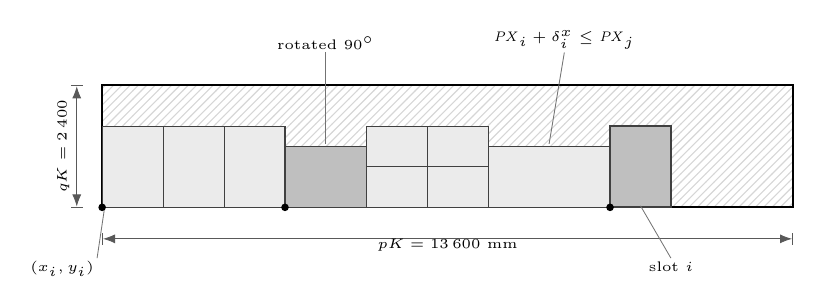
\begin{tikzpicture}[x=0.645cm, y=0.645cm, >=Latex,
  fp/.style={draw=black!75, fill=black!8, line width=0.4pt},
  hl/.style={draw=black!75, fill=black!25, line width=0.4pt},
  tny/.style={font=\tiny, align=center, inner sep=1pt},
  led/.style={black!55, line width=0.3pt}]
  % trailer floor, 13.6 x 2.4 (decimetres of the real 13 600 x 2 400 mm)
  \fill[pattern=north east lines, pattern color=black!16]
     (0,0) rectangle (13.6,2.4);
  \draw[line width=0.7pt] (0,0) rectangle (13.6,2.4);

  % 1200 x 1600 footprints
  \foreach \x in {0,1.2,2.4} \draw[fp] (\x,0) rectangle ++(1.2,1.6);
  % one rotated 90 degrees: 1600 x 1200
  \draw[hl] (3.6,0) rectangle ++(1.6,1.2);
  % 1200 x 800 footprints
  \foreach \x/\y in {5.2/0, 5.2/0.8, 6.4/0, 6.4/0.8}
     \draw[fp] (\x,\y) rectangle ++(1.2,0.8);
  % 2400 x 1200
  \draw[fp] (7.6,0) rectangle ++(2.4,1.2);
  % the lifted slot i
  \draw[hl, line width=0.8pt] (10.0,0) rectangle ++(1.2,1.6);

  % bottom-left corners
  \foreach \x/\y in {0/0, 3.6/0, 10.0/0} \fill[black] (\x,\y) circle (0.075);

  % dimensions
  \draw[|<->|, black!65, line width=0.3pt] (0,-0.62) -- (13.6,-0.62);
  \node[tny, anchor=north] at (6.8,-0.56) {$pK=13\,600$ mm};
  \draw[|<->|, black!65, line width=0.3pt] (-0.50,0) -- (-0.50,2.4);
  \node[tny, rotate=90, anchor=south] at (-0.58,1.2) {$qK=2\,400$};

  % annotations outside the floor, with leaders
  \node[tny, anchor=south] (rot) at (4.4,3.05) {rotated $90^{\circ}$};
  \draw[led] (rot.south) -- (4.4,1.25);
  \node[tny, anchor=south] (nov) at (9.1,3.05)
     {$\mathit{PX}_{i}+\delta^{x}_{i}\le \mathit{PX}_{j}$};
  \draw[led] (nov.south) -- (8.8,1.25);
  \node[tny, anchor=north west] (sl) at (10.7,-1.00) {slot $i$};
  \draw[led] (sl.north) -- (10.6,0.03);
  \node[tny, anchor=north east] (bl) at (-0.10,-1.00) {$(x_{i},y_{i})$};
  \draw[led] (bl.north east) -- (0.04,-0.06);
\end{tikzpicture}
\caption{the floor, \eqref{bp:PP-nonov-x1}--\eqref{bp:PP-cont-x}}
\label{fig:truck-floor}
\end{subfigure}\hfill
\begin{subfigure}[b]{0.30\textwidth}
\centering
\tdplotsetmaincoords{72}{128}
\begin{tikzpicture}[tdplot_main_coords, scale=0.70, >=Latex,
  tny/.style={font=\tiny, align=left, inner sep=1pt}]
  % four homogeneous layers in one slot, two shades: the per-slot assignment
  \drawblock{0}{0}{0}{1.2}{1.6}{0.62}{stkA}{0}{0}{1}
  \drawblock{0}{0}{1.24}{1.2}{1.6}{0.62}{stkB}{0}{0}{1}
  % height budget
  \draw[|<->|, black!70, line width=0.3pt] (1.55,0,0) -- (1.55,0,2.48);
  \node[tny, anchor=west] at (2.90,0,1.55)
     {$\sum_{r} r_{pr}\ell_{ir}$\\ $\le rK$};
  % crush cap at the base
  \node[tny, anchor=north] at (0.6,0.8,-0.30)
     {$\sum_{n}w_{n}v_{in}\le W^{\max}$};
  \node[tny, anchor=south] at (0.6,0.8,2.95)
     {$v_{in}$: two products,\\ one per layer};
\end{tikzpicture}
\caption{one slot, \eqref{eq:col-height} and \eqref{eq:col-crush}}
\label{fig:truck-stack}
\end{subfigure}
\caption{What the pricing problem designs: footprints placed on the
floor without overlap, each slot a stack of homogeneous layers under the
height budget \eqref{bp:PP-height} and the per-slot crush cap, the load
assigned to the slots, $b_{\omega n}=\sum_{i\le m}v_{in}$, and the
truck full by volume \emph{or} by payload
\eqref{bp:PP-util}--\eqref{bp:PP-utilw}.}
\label{fig:truck}
\end{figure}


\paragraph{What pricing cannot return.}
The pricing objective is linear in the image, so an optimum can
always be taken at an extreme point of $\operatorname{conv}(\Omega^{g})$,
and a load in its relative interior is never the unique optimum: a
balanced load inside the hull is matched by a fractional blend of
single-commodity trucks, and no dual vector asks for it. Such interior loads are what an
integer plan needs when a period's demand does not decompose into full
trucks; the construction of Section~\ref{sec:relaxfix-flow} builds
them directly, and branching on the fleet moves the duals so that
pricing is asked for loads the pool lacks.

\section{Branching, with the flow-first construction inside it}
\label{sec:branching}

The search branches on quantities the master already prices, so every
child is a set of robust rows and the pricing problem is never changed.
Transport costs $cK\cdot X$ with $X=\sum_{g,t}n_{gt}$ the total fleet,
and moving freight between periods can compensate a bound on a single
period's dispatches or deliveries at the price of one period's holding
cost but not a bound on $X$; the search therefore branches on $X$ first
and then, inside $X=X^{\star}$, on the fleet vector. Bounding a single
$\lambda^{g}_{\omega t}$ instead would exclude a column from the
subproblem \autocite{Vanderbeck2000OnIntegerProgramming}, and with
many columns differing in a single RTI the relaxation would only shift
the same fractional weight one column over. Master, pricing problem,
construction and tree together form BP-3D-SCPTOP
(Algorithm~\ref{alg:bp3d}).

\paragraph{Level 1: the total fleet.}
Around an incumbent of total $X^{\star}$, the regions
$X\ge X^{\star}+1$, $X=X^{\star}$ and $X\le X^{\star}-1$ partition the
space. The first costs a whole truck and is usually pruned by bound;
the second fixes transport, so everything in it is inventory
allocation; the third is the only one that can beat the incumbent
outright, and it is expanded first. A plan found inside an inequality
region splits it the same way, so level 1 recurses.

\paragraph{Level 2: the fleet vector, inside $X=X^{\star}$.}
Fix an order on the pairs $(g,t)$. Any plan in the region differs from
the incumbent's fleet vector $\mathbf{n}^{\star}$ at a first index $j$,
or nowhere, so branching there gives the disjoint and exhaustive
children
\begin{equation}
n_{j}\le n^{\star}_{j}-1,
\qquad
n_{j}= n^{\star}_{j},
\qquad
n_{j}\ge n^{\star}_{j}+1,
\label{eq:murty}
\end{equation}
with the equality child partitioned again at $j+1$
\autocite{Murty1968AnAlgorithm} and expanded first, always around the
plan constructed at the node.

\paragraph{Pruning, bounds and what may be claimed.}
A node is a region imposed on the RMP as fleet rows. Its pool LP is a
filter; where the filter allows and the policy admits the node, the
region is certified (Algorithm~\ref{alg:certify}) and pruned if the
certified value reaches the incumbent, and otherwise it keeps its
parent's bound. An infeasible node relaxation is not a proof that a
region is empty, stock non-negativity being rigid; only arithmetic is:
the fleet box, availability caps telescoped from the sending rows, and
the constants of \eqref{eq:covercut} read as a requirement floor. Under
3D loading every region's certificate comes from the volumetric
relaxation with the region's fleet rows applied, which
Proposition~\ref{prop:inclusion} covers. The incumbent is the cheapest
verified plan any construction found and the global bound the minimum
over the frontier. Optimality is claimed only when the root is
certified, no region remains open or merely bounded, and the incumbent
meets the global bound; no run here meets those conditions. A third
level, on deliveries, is disabled in every run reported, so a
full-depth leaf is covered by a certificate rather than split again.

\begin{algorithm}[!htb]
\caption{BP-3D-SCPTOP: branch and bound over the fleet vector, with
\textsc{Construct} as primal heuristic and \textsc{Certify} as bound.}
\label{alg:bp3d}
\begin{algorithmic}[1]
\State $\bar\Omega\gets$ one maximally full single-commodity truck per commodity
   and direction, each verified
\State $\mathrm{LB}_{0}\gets\textsc{Certify}(\bar\Omega,\text{root})$;
   $(\bar z,\mathbf{n}^{\star},\bar\Omega)\gets\textsc{Construct}(\bar\Omega,\text{root})$;
   $X^{\star}\gets\sum_{g,t}n^{\star}_{gt}$
\State $\mathcal{S}\gets[\,X\ge X^{\star}+1,\; X=X^{\star},\; X\le X^{\star}-1\,]$
   \Comment{a stack: the region that can beat the incumbent is popped first}
\While{$\mathcal{S}\ne\emptyset$ and time remains}
   \State $\mathcal{R}\gets$ pop $\mathcal{S}$; impose it on the RMP as fleet rows
   \If{$\mathcal{R}$ is refuted arithmetically} \State \textbf{continue}
      \Comment{fleet box, availability, requirement} \EndIf
   \State $\tilde z\gets$ LP over $\bar\Omega$ inside $\mathcal{R}$
      \Comment{over-estimates the region's LP: a filter, never a bound}
   \If{$\tilde z\ge\bar z$ and the policy certifies $\mathcal{R}$}
      \State $(\mathrm{LB}_{\mathcal{R}},\text{proved})\gets
             \textsc{Certify}(\bar\Omega,\mathcal{R})$
      \If{$\mathrm{LB}_{\mathcal{R}}\ge\bar z$} \State \textbf{continue}
         \Comment{pruned} \EndIf
      \State record $\mathrm{LB}_{\mathcal{R}}$ as an open bound
   \Else \State $\mathcal{R}$ carries its parent's bound \EndIf
   \State $(z,\hat{\mathbf{n}},\bar\Omega)\gets\textsc{Construct}(\bar\Omega,\mathcal{R})$
      \Comment{its columns join the shared pool whatever it returns}
   \If{no plan} \State price under $\mathcal{R}$'s duals and construct once
      more; \textbf{continue} if still none \EndIf
   \If{$z<\bar z$} \State $(\bar z,\mathbf{n}^{\star})\gets(z,\hat{\mathbf{n}})$
      \Comment{new incumbent} \EndIf
   \If{$\mathcal{R}$ does not fix $X$}
      \State push the three regions of level 1 around
            $\sum_{g,t}\hat n_{gt}$ \Comment{level 1 recurses}
   \ElsIf{the Murty depth $j$ is below the cap (Table~\ref{tab:impl})}
      \State push the three children \eqref{eq:murty} at the $j$-th pair,
             around $\hat{\mathbf{n}}$, equality last
   \EndIf
\EndWhile
\ForAll{$\mathcal{R}$ still on $\mathcal{S}$, while a reserve of time remains}
   \State filter by the pool LP; certify the survivors; record their bounds
   \Comment{the frontier}
\EndFor
\State $\mathrm{LB}\gets\max\{\mathrm{LB}_{0},\,
   \min\text{ over the open and frontier bounds}\}$, capped at $\bar z$
   \Comment{a dropped region contributes $\mathrm{LB}_{0}$}
\State verify every dispatched truck of the incumbent against
   \eqref{eq:col-geom}--\eqref{eq:col-agg}
\State \Return $(\bar z,\mathrm{LB})$; optimality is claimed only if
   $\mathrm{LB}_{0}$ was proved, $\mathcal{S}=\emptyset$, no region was
   dropped and $\bar z=\mathrm{LB}$
\end{algorithmic}
\end{algorithm}


\subsection{The initial pool}
\label{sec:initcols}
The search starts from one maximally full truck per commodity and
direction, obtained by pricing that commodity alone with every other
capped at zero (volumetrically, by filling to capacity); no mixed loads
are seeded.

\subsection{The flow-first construction}
\label{sec:relaxfix-flow}

The primal heuristic decides how much moves and how many trucks carry
it before it builds any truck. Pricing returns only extreme loads, so
the mixed loads a plan needs must come from elsewhere: the construction
fixes integer deliveries and fleet over \emph{continuous} column
weights, then cuts each period's deliveries into legal trucks. It runs
inside the region $\mathcal{R}$ of its node, on a fresh copy of the RMP
(Algorithm~\ref{alg:construct}).

\begin{enumerate}
\item \emph{Restricted master.} The LP over the pool, inside
  $\mathcal{R}$, gives the duals and the fractional point.

\item \emph{Aggregate integer master.} The dispatch totals $n_{gt}$
  become integer variables and $\overline{V}_{nt},
  \overline{V^{\mathrm{e}}}_{rt}$ integer, the column variables stay
  continuous, $\mathcal{R}$ is imposed on the $n_{gt}$, and under 3D
  loading the aggregate forms of
  \eqref{eq:stackrows}--\eqref{eq:fibrerows} are added. The objective is
  decided here, without a pricing call; artificial slack above a
  tolerance abandons the node.

\item \emph{Partition, as a cover.} Each period's integer deliveries
  $Q^{\star}_{gt}$ are covered by $n^{\star}_{gt}$ legal trucks, an
  integer programme over per-truck commodity counts $a_{kc}$:
  \begin{align}
    \min\;\;&\sum_{c}\gamma_{gc}\Bigl(\sum_{k}a_{kc}-Q^{\star}_{gtc}\Bigr)
      \label{eq:part-obj}\\
    \text{s.t.}\;\;&\sum_{k}a_{kc}\;\ge\;Q^{\star}_{gtc} &&\forall c
      \label{eq:part-cover}\\
    &\textstyle\sum_{c}\gamma_{gc}a_{kc}\le\Gamma_{K},\qquad
     \sum_{c}w_{c}a_{kc}\le pK^{w} &&\forall k
      \label{eq:part-cap}\\
    &\textstyle\sum_{c}\gamma_{gc}a_{kc}\ge\alpha\Gamma_{K}\theta_{k},\qquad
     \sum_{c}w_{c}a_{kc}\ge\alpha pK^{w}(1-\theta_{k}) &&\forall k
      \label{eq:part-floor}\\
    &\textstyle\sum_{c}w_{c}a_{kc}\;\ge\;\sum_{c}w_{c}a_{k+1,c}
      &&\forall k<n^{\star}_{gt}
      \label{eq:part-sym}\\
    &a_{kc}\in\{0,\dots,\bar u_{gc}\},\qquad \theta_{k}\in\{0,1\}.\nonumber
  \end{align}
  with $\theta_{k}$ selecting the resource on which part $k$ is full and
  $\bar u_{gc}$ the placeability cap below. If $n^{\star}_{gt}$ parts
  cannot be formed, $n^{\star}_{gt}+1$ and $+2$ are tried.

\item \emph{Integer master over pool plus parts}, warm-started with the
  partition; its solution is the node's plan.
\end{enumerate}

\noindent The partition must be a cover: a fractional blend of legal
loads need not split into legal loads for any number of trucks, floor
area being consumed in whole footprints. A cover is sound because every
part is a legal column, step~4 may dispatch fewer of them than were
built, and over-delivery is feasible.

\begin{algorithm}[!htb]
\caption{$\textsc{Construct}(\bar\Omega,\mathcal{R})$ --- the flow-first
relax and fix. Line 4, the rows of line 12 and lines 15--27 apply under
3D loading only. $\varepsilon_{2}$
is step~2's relative MIP gap and \emph{tol} the tolerance above which
artificial slack means the region admits no plan over this pool.}
\label{alg:construct}
\begin{algorithmic}[1]
\State $\bar\Omega'\gets$ a fresh copy of the RMP over $\bar\Omega$
   \Comment{not the node's own LP: step 2 changes variable types}
\State solve $\mathrm{LP}(\bar\Omega',\mathcal{R})$
   \Comment{duals $\pi,\mu$ and the fractional point the node stands on}
\State make $n_{gt},\overline{V}_{nt},\overline{V^{\mathrm{e}}}_{rt}$ integer;
   keep $\lambda$ continuous; impose $\mathcal{R}$ on $n_{gt}$ and on $\lambda$
\State add the aggregate forms of \eqref{eq:stackrows}--\eqref{eq:fibrerows}
   \Comment{3D only; layer coefficient $=$ the height count, the crush
      limit being its own row}
\State solve to relative gap $\varepsilon_{2}$
\If{no solution, or artificials $>$ tol}
   \State \Return $\bot$ \Comment{node abandoned; the region is infeasible over this pool} \EndIf
\State $(Q^{\star},n^{\star})\gets$ the integer deliveries and fleet
\ForAll{$(g,t)\in G\times T$}
   \For{$m=n^{\star}_{gt},\,n^{\star}_{gt}+1,\,n^{\star}_{gt}+2$ while
        $\mathcal{R}$ allows}
      \State solve $\textsc{Partition}(Q^{\star}_{gt},m)$,
             \eqref{eq:part-obj}--\eqref{eq:part-sym}, with $\bar a_{gc}$ as
             variable bounds and, in 3D,
             \eqref{eq:stackrows}--\eqref{eq:fibrerows} per part
      \State \textbf{break} if feasible
      \Comment{a timeout is not a proof of infeasibility}
   \EndFor
   \ForAll{parts $a_{k}$ of the cover}
      \State $(\text{verdict},\text{layout})\gets\textsc{Pack}(a_{k})$
      \If{placeable} \State verify the layout;
          $\bar\Omega\gets\bar\Omega\cup\{(a_{k},\text{layout})\}$ \EndIf
      \If{\emph{proved} unplaceable} \State bisect $\sigma\in(0,1]$ and cut
          every load dominating $\lfloor\sigma a_{k}\rfloor$
          \Comment{validity} \EndIf
      \If{undecided} \State exclude $a_{k}$ as a single point
          \Comment{heuristic restriction, never validity} \EndIf
   \EndFor
   \State re-solve the partition if a cut was written and rounds remain
\EndFor
\State $\bar\Omega\gets\bar\Omega\cup\{\text{the parts}\}$; solve the integer
   master over $\bar\Omega$, warm-started with the partition
\State \Return $(z,\hat{\mathbf{n}},\bar\Omega)$
   \Comment{the parts are kept even when no plan is returned}
\end{algorithmic}
\end{algorithm}


\subsection{The construction under 3D loading}
\label{sec:geo3d}

Under 3D loading each part must also satisfy
\eqref{eq:col-geom}--\eqref{eq:col-agg}. The partition programme is a
relaxation of placeability, so each part is submitted to a placeability
oracle; everything rests on placeability being \emph{downward closed}:
removing units from a layout leaves a layout.

\paragraph{Deciding placeability.}
A constructive \emph{shelf design}, a small integer programme laying
the part's stacks in shelves along the trailer, supplies most positive
answers, and its layout passes the independent verifier of
Section~\ref{sec:res-setup}. Refutations come from decoupling: a stack
carries one footprint class, so a load within the payload is placeable
if and only if, for each class $f$, the least number
$\underline{s}_{f}$ of class-$f$ stacks its units need can be placed on
the floor as rectangles. The least count is a small cutting-stock
problem per class, and the placement is decided exactly by a
position-indexed model over the normal patterns of the floor
\autocite{ChristofidesWhitlock1977,Beasley1985}; an infeasible placement
at a lower bound on $\underline{s}_{f}$ already refutes.

\paragraph{Cuts.}
A part \emph{proved} unplaceable yields a \emph{dominance cut}
forbidding every load that dominates it, valid by downward closure and
written at the smallest point $\lfloor\sigma a\rfloor$ of its ray,
$\sigma\in(0,1]$, still proved unplaceable. A part left
\emph{undecided} is excluded as a single point: a restriction of the
heuristic, never a validity claim. The largest placeable count of each
commodity is bisected once per run and handed to the partition as
$\bar u_{gc}$.

\paragraph{Necessary conditions of placeability as rows.}
Per truck $k$ and footprint class $f$ --- a stack type $h$ of
Section~\ref{sec:model}, with $p_{f}=p_{h}$ and $q_{f}=q_{h}$ --- the
partition carries an integer number of stacks
$s_{kf}\le\lfloor pK\cdot qK/p_{f}q_{f}\rfloor$ with the crush limit,
the height budget and the floor area imposed:
\begin{equation}
\sum_{c\in f}w_{c}a_{kc}\le W^{\max}s_{kf},
\qquad
\sum_{c\in f}r_{gc}\,a_{kc}\le rK\,s_{kf},
\qquad
\sum_{f}p_{f}q_{f}\,s_{kf}\le pK\cdot qK ,
\label{eq:stackrows}
\end{equation}
where a class carries one RTI type the height row takes the
height-limited count, $\sum_{c\in f}a_{kc}\le\lfloor
rK/r_{gr}\rfloor s_{kf}$. It also carries the finer conditions by which
the oracle refutes a load. With $C_{f}$ the commodities of class $f$
and $L^{\max}_{f}$ the most units of them one stack can hold, a
two-resource knapsack under $rK$ and $W^{\max}$,
\begin{equation}
\begin{gathered}
\sum_{\substack{c\in C_{f}\\ w_{c}\ge\xi}}a_{kc}\le
  \Bigl\lfloor\frac{W^{\max}}{\xi}\Bigr\rfloor s_{kf}
  \;\;\forall\xi\in\{w_{c}\}_{c\in C_{f}},
\qquad
\sum_{\substack{c\in C_{f}\\ r_{gc}\ge\xi}}a_{kc}\le
  \Bigl\lfloor\frac{rK}{\xi}\Bigr\rfloor s_{kf}
  \;\;\forall\xi\in\{r_{gc}\}_{c\in C_{f}},
\\
\sum_{c\in C_{f}}a_{kc}\le L^{\max}_{f}\,s_{kf},
\end{gathered}
\label{eq:geomrows}
\end{equation}
the height thresholds being written only where a class carries more
than one RTI type; and, with $s_{kf}=s^{0}_{kf}+s^{1}_{kf}$ split into
stacks laid with $p_{f}$ along the trailer's length $pK$ and along its
width $qK$,
\begin{equation}
\sum_{f}\bigl(u_{1}(p_{f})\,q_{f}\,s^{0}_{kf}+u_{1}(q_{f})\,p_{f}\,s^{1}_{kf}\bigr)
  \le U_{1}\,qK,
\qquad
\sum_{f}\bigl(p_{f}\,u_{2}(q_{f})\,s^{0}_{kf}+q_{f}\,u_{2}(p_{f})\,s^{1}_{kf}\bigr)
  \le pK\,U_{2},
\label{eq:fibrerows}
\end{equation}
for every pair $(u_{1},U_{1})$ on $pK$ and $(u_{2},U_{2})$ on $qK$ of a
finite family of \emph{dual-feasible functions}, $(u,U)$ being one on a
length $C$ when $\sum_{i}x_{i}\le C$ implies $\sum_{i}u(x_{i})\le U$
\autocite{FeketeSchepers2001,Clautiaux2010Survey}: the identity
($U=C$, the area row), the thresholds $[x\ge\ell]$ at the footprint
lengths that occur ($U=\lfloor C/\ell\rfloor$), and the scalings
$\lfloor jx/C\rfloor$ ($U=j$, $j\le12$). Every row holds for every
placeable truck with $s_{kf}$ and its split read off the truck's own
layout --- a stack bears at most $W^{\max}$ and $rK$, and
\eqref{eq:fibrerows} is the conservative-scale argument of
\textcite{FeketeSchepers2004} with one dimension unscaled --- so the
rows remove only parts the oracle would refuse. Step~2 carries their
sum over the period's trucks, the right-hand sides of
\eqref{eq:fibrerows} multiplied by $n_{gt}$. They are implied in the
pricing problem and in the master, whose points and columns are
placeable, but not in the volumetric relaxation that supplies the
bounds; in the method they cut only the free integer vectors of
steps~2 and~3.

\section{Computational results}
\label{sec:results}

\subsection{Setup}
\label{sec:res-setup}

The method is implemented in Julia with JuMP and solves every model
with Gurobi; Appendix~\ref{appendix:impl} describes the implementation
and the settings of every run, and the code and data are available at
\Pending{[repository URL]}. Every 3D plan below is re-derived
from its dispatch list alone and checked truck by truck against
\eqref{eq:col-geom}--\eqref{eq:col-agg} by a routine independent of
the search and of the oracle that built the column, re-deriving each
slot's weight from the products it carries. A \emph{gap} is always
$(z-\mathrm{LB})/z$. Outside Section~\ref{sec:res-bench} and
Appendix~\ref{appendix:bench}, LB is the method's own certified bound;
there, it is the best valid bound for the 3D problem on the instance,
the method's own or the compact volumetric model's dual bound,
whichever is larger. Table~\ref{tab:quantities} defines the other
quantities.

% Generator: src/rti3d/instance.py generate_instance and design_grid (branch
% final-3d); experiments/gen_instances.py, seeds 1000-1035 (meta.seed in
% instances/I_*.json).  Nominal RTI volume Gamma_K / v; products assigned to
% types in turn (rtis[j % n_rti]); n_foot = min(admissible, max(2, 1 +
% |R| // 2)) footprints: 2 at |R| = 2 and 3, 3 at |R| = 4 (checked on the 36
% JSONs).  Content weight 340 kg x (type volume / nominal) x U(0.75, 1.25),
% so it does not scale with v: median w_full - w_tare 368 / 371 / 366 kg at
% v = 60 / 90 / 120 over the 36 instance files.  trucks_per_period 2.5 in
% every file's meta.
\paragraph{Instances.}
Instances are named $I\_|N|\_|T|\_|R|\_v$, with $|R|$ the number of
RTI types and $v$ the number of erected RTIs that fill one truck by
volume, an RTI's nominal volume being $\Gamma_{K}/v$. Footprints come
from the industrial catalogue, from $800\times600$ to $2400\times1200$
mm, with heights quantised to $50$ mm and bounded so that at least two
layers fit under the roof; demand deviates $\pm10\%$ from its mean, and
content weight by $\pm25\%$ between products sharing a type, which
makes the crush limit depend on the period's mix. There are two sets.
In the first, every instance has $|R|=2$ and $v=90$. The smallest,
$I\_8\_5\_2\_90$, consumes
roughly $2.5$ truckloads per period; the other six pair $(|N|,|T|)$
with $2.5$, $5$ or $8$ truckloads per period, the name's suffix being
that figure times ten: $(8,10)$, $(12,12)$ and $(16,15)$ at $2.5$,
$(16,15)$ and $(24,20)$ at $5$, and $(24,20)$ at $8$. The five solved
in 3D (Table~\ref{tab:3d-onecommit}), from $I\_8\_5\_2\_90$ to
$I\_24\_20\_2\_90\_k50$, form the \emph{size ladder}, each instance a
\emph{rung}. The second set is a full factorial \emph{benchmark} of
$36$ instances, $|N|\in\{4,8\}$, $|T|\in\{5,10\}$, $|R|\in\{2,3,4\}$
and $v\in\{60,90,120\}$, each consuming roughly $2.5$ truckloads per
period; its $I\_8\_5\_2\_90$ is the ladder's first rung. Products are
assigned to the RTI types in turn, and types share footprints from
$|R|=3$ on (two footprints for $|R|\le3$, three for $|R|=4$), so a
stack may mix types across layers. Content weight does not scale with
$v$, so a smaller $v$ means larger containers of similar weight. The
truck is a semi-trailer, $13600\times2400\times3000$ mm,
payload $24$ t, $W^{\max}=1200$ kg, $\alpha=0.55$, $cK=1000$ per
dispatch, $lt=1$, one period of coverage stock.

\begin{table}[!htbp]
\centering
\small
\caption{What each reported quantity means.}
\label{tab:quantities}
\begin{tabular}{@{}lp{0.80\textwidth}@{}}
\toprule
$z$ & Cost \eqref{eq:MPObjective} of the plan returned, which carries
  no artificial slack; an upper bound on the optimum. \\
trucks & $\sum_{g,t}n_{gt}$ for that plan. \\
LB & For the method, the certified bound of Section~\ref{sec:bounds},
  printed only where every pair of its sweep was proved, or the
  Lagrangian bound of that section where it is larger; for a compact
  model, the solver's dual bound at its stop. \\
gap & $(z-\mathrm{LB})/z$ against the method's own bound, except in
  Section~\ref{sec:res-bench} and Appendix~\ref{appendix:bench}, where
  LB is the larger of the method's and the compact volumetric model's
  bounds; an optimality gap only to the extent that bound is tight. \\
stop & \textsc{optimal}, \textsc{time\_limit} or \textsc{mem\_limit};
  after a time or memory stop the row's time is the budget. \\
nodes / open & Tree nodes opened; regions still unexpanded at the
  deadline. A run with open regions has not searched the space, and one
  with none has not refuted it either if a region was closed with a
  bound below the incumbent. \\
dropped & Regions abandoned without a certificate of their own (for
  instance, no plan was constructed in them); only the root's bound
  covers them. \\
verified & Dispatched trucks found legal by the independent check of
  Section~\ref{sec:res-setup}, out of the number dispatched. \\
$\Delta z$ & The cost of one method relative to another on the same
  instance, with the denominator named where it appears. \\
\bottomrule
\end{tabular}
\end{table}


\subsection{The volumetric problem}
\label{sec:res-vol}

% Method rows: results/julia/parity_vol.csv, the volumetric parity campaign of
% 2026-10-27 -- the Julia implementation on all six instances at the compact
% reference's own budget (3600 s, 20 GB, 10 threads), commit 10e633c.  Every
% row carries root_proved=true, so none of them rests on the unproved-root
% bound defect fixed in e85c70c; that fix changes only the case where no
% certificate exists, and here one always does.  The t column is the `seconds`
% field, the method's own wall clock.  It lands at 3062-3133 s, not 3600:
% tree.jl:601-602 gives the search (1 - frontier_share) * time_limit = 3060 s
% and reserves the remainder for the frontier sweep, which returns in 2.3 to
% 72.5 s on these six.  The shortfall is the reserve going unspent, not a
% phase refused.
% Compact rows: results/compact_ref/compact_ref_<instance>.json, each with its
% own config block: 3600 s (1800 on I_8_5_2_90), MIP gap 0, 10 threads, 20 GB,
% seed 0.
% NOTE on the compact t column: every row prints the files' `wall` field
% (0.198167, 3268.92, 1349.52, 1121.83, 2093.27, 2403.21), not `runtime`
% (0.185, 3242.96, 1349.44, 1112.70, 2087.63, 2399.01).  One field for the
% whole column, and `wall` is the comparable one: the method's own time is
% wall-clock, so setting it against the compact model's solver time would
% flatter the method by the model-build time it does not charge itself.  The
% two fields differ by under 1% on every row, so nothing in the comparison
% turns on the choice -- but a column read off two fields is indefensible.
\begin{table}[!htbp]
\centering
\small
\caption{The method under its volumetric oracle against SCPTOP, the
compact formulation of the volumetric problem of
Appendix~\ref{appendix:A}: a check on the method where an independent
optimum exists. $z$ is the incumbent at the stop; \textsc{opt} marks a
proved optimum, $^{\mathrm{m}}$ a stop on the memory cap,
$^{\mathrm{t}}$ a stop on time. ``bound'' is Gurobi's dual bound for
the compact model and the certified bound of Section~\ref{sec:bounds}
for the method. $\Delta z=(z_{\mathrm{method}}-z_{\mathrm{compact}})/
z_{\mathrm{compact}}$, negative when the method's plan is cheaper. Both
sides had $3\,600$ s ($1\,800$ s for the compact model on
$I\_8\_5\_2\_90$, which it solved in $0.2$ s), $20$ GB and ten
threads, the method's column generation apart (Appendix~\ref{appendix:impl}).
A volumetric column carries no layout, so no plan here is verified
truck by truck.}
\label{tab:volumetric}
\resizebox{\textwidth}{!}{%
\begin{tabular}{lrrrrlrrrrr}
\toprule
 & \multicolumn{4}{c}{compact SCPTOP} & \multicolumn{4}{c}{BP-3D-SCPTOP (volumetric oracle)} & & \\
\cmidrule(lr){2-5}\cmidrule(lr){6-9}
Instance & $z$ & bound & trucks & $t$ (s) & $z$ & bound (cert.) & trucks & $t$ (s) & $\Delta z$ (\%) & tighter bound \\
\midrule
$I\_8\_5\_2\_90$ & 18\,796.96\,\textsc{opt} & 18\,796.96 & 12 & 0.198 & 18\,796.96$^{\mathrm{t}}$ & 18\,795.56 & 12 & 3064 & $0.0000$ & 18\,796.96 (compact) \\
$I\_8\_10\_2\_90\_k25$ & 38\,855.65$^{\mathrm{m}}$ & 38\,851.93 & 26 & 3269 & 38\,853.17$^{\mathrm{t}}$ & 38\,791.19 & 26 & 3062 & $-0.0064$ & 38\,851.93 (compact) \\
$I\_16\_15\_2\_90\_k25$ & 68\,139.17\,\textsc{opt} & 68\,139.17 & 45 & 1350 & 68\,139.21$^{\mathrm{t}}$ & 68\,131.48 & 45 & 3117 & $+0.0001$ & 68\,139.17 (compact) \\
$I\_16\_15\_2\_90\_k50$ & 134\,346.91$^{\mathrm{m}}$ & 133\,417.47 & 89 & 1122 & 134\,507.47$^{\mathrm{t}}$ & 133\,484.56 & 89 & 3073 & $+0.1195$ & 133\,484.56 (method) \\
$I\_24\_20\_2\_90\_k50$ & 200\,266.21$^{\mathrm{m}}$ & 199\,518.04 & 137 & 2093 & 200\,048.69$^{\mathrm{t}}$ & 200\,013.57 & 137 & 3071 & $-0.1086$ & 200\,013.57 (method) \\
$I\_24\_20\_2\_90\_k80$ & 282\,101.77$^{\mathrm{m}}$ & 280\,823.53 & 189 & 2403 & 281\,233.28$^{\mathrm{t}}$ & 280\,910.22 & 188 & 3133 & $-0.3079$ & 280\,910.22 (method) \\
\bottomrule
\end{tabular}}
\end{table}


The volumetric problem of Appendix~\ref{appendix:A} is the only part of
the problem with an independent optimum, because a compact formulation
of it, SCPTOP, solves exactly on the smaller instances; Table~\ref{tab:volumetric}
therefore checks whether the method arrives where it should, at the
same $3\,600$ s, $20$ GB and ten threads. It does. On $I\_8\_5\_2\_90$
it returns the proved optimum $18\,796.96$, to the cent, with twelve
trucks; on $I\_16\_15\_2\_90\_k25$ it returns $68\,139.21$ against a
proved $68\,139.17$ at forty-five trucks, $0.0001\%$ above the optimum,
with its own certified bound $0.0113\%$ below it. Where the compact
model works it is far the faster, at $0.2$ s and $1\,350$ s against
the method's roughly $3\,070$ s.

On the four instances where the compact model exhausts its memory cap,
costs agree within $0.31\%$, with the same fleet on three and one truck
fewer for the method on $I\_24\_20\_2\_90\_k80$; the method's plan is
cheaper on three and dearer on one, by $0.1195\%$ on
$I\_16\_15\_2\_90\_k50$, where it left its own interval $0.76\%$ wide.
On the three largest instances its certified bound is the tighter, by
$67$, $496$ and $87$ cost units. On $I\_12\_12\_2\_90\_k25$ the method
certifies $52\,105.31$, valid for the 3D problem by
Proposition~\ref{prop:inclusion}, $274$ s into its run, where the
compact volumetric model stood at a dual bound of $51\,944.22$ when its
$600$ s expired: the decomposition's bound is $0.310\%$ tighter,
relative to the compact bound.
% 52105.31 at 274.0 s: results/julia/final/ladder_3d_final.log line 699
% ("volumetric relaxation LB 52105.31 proved=true"), the ladder's third rung.

\subsection{The 3D problem}
\label{sec:res-3d}

% Source: results/julia/final/ladder_3d_final.csv (one row per rung) and its
% trace results/julia/final/ladder_3d_final.log, both on branch final-3d of the
% outer repository, committed at 4c7471e.  Launcher
% julia/scripts/ladder_3d_final.sh at f4c3b18 (tag final-3d-2026-11-04);
% src_tree e4830fe and load_path include on every row.  Run on the workstation
% as systemd unit rti-final, alone, 2026-11-04 14:22-16:32: mode 3d, 10
% threads, mem_gb 20, certify_regions ratchet, root_cg_share 0.15, stop_early
% off, no seed set, geom_rows both, ip_tl = time_limit/6 (150/150/300/300/600).
% Columns, all from the CSV unless stated:
%   z = incumbent (= plan_cost); trucks;
%   verified = trucks, complaints = 0 on every row (verify_plan plus
%     verify_column on every dispatched truck, julia/src/tree.jl:1493-1520);
%   LB = global_lb = root_lb, root_proved true, bound_source "volumetric
%     relaxation (by inclusion)"; gap = gap_pct (0.0075 / 0.1628 / 0.022 /
%     14.5186 / 10.686);
%   root (t) = the log's "root plan" line: 18797.59 at 142.0 s, 38867.74 at
%     154.4 s, 52215.42 at 298.4 s, 92251.99 (X=67) at 948.4 s, 223944.2
%     (X=156) at 2771.5 s; tree = (root - z)/root;
%   nodes; dropped = regions_dropped; open = open_regions (row 4 also has
%     regions_unbounded 4); wall = seconds (765.03 / 770.47 / 1547.81 /
%     1533.82 / 3093.57).
% proved = false on every row.  pack_undecided = 0 on every row.
\begin{table}[!htbp]
\centering
\small
\caption{BP-3D-SCPTOP on the size ladder. \emph{root} is the plan the
construction returns before any node is popped, with the time it
arrived, and \emph{tree} the improvement the search then makes on it,
relative to the root plan's cost. \emph{open} and \emph{dropped} are as
in Table~\ref{tab:quantities}; on row 4, four of the seven open regions
carry no bound of their own. LB is the certified volumetric bound,
valid for 3D by Proposition~\ref{prop:inclusion} and loose wherever the
crush limit binds, so the gaps on the last two rows are not optimality
gaps; on rows 2 and 4 the compact volumetric model supplies tighter
valid bounds ($38\,851.93$ and $68\,139.17$,
Table~\ref{tab:volumetric}). The method proves no row optimal; row 1's
plan attains the compact volumetric optimum ($18\,796.96$), which proves
it optimal by inclusion. The wall clock stops short of the budget because
$15\%$ of it is reserved for the frontier sweep.}
\label{tab:3d-onecommit}
\begin{tabular}{lrrlrr}
\toprule
Instance & $z$ & trucks & verified & LB (cert.) & gap \\
\midrule
$I\_8\_5\_2\_90$        & \textbf{18\,796.96} & 12  & 12 / 12   & 18\,795.56 & $0.0075\%$ \\
$I\_8\_10\_2\_90\_k25$  & 38\,854.44 & 26  & 26 / 26   & 38\,791.19 & $0.163\%$ \\
$I\_12\_12\_2\_90\_k25$ & 52\,116.76 & 34  & 34 / 34   & 52\,105.31 & $0.022\%$ \\
$I\_16\_15\_2\_90\_k25$ & 79\,703.31 & 55  & 55 / 55   & 68\,131.48 & $14.5\%$ \\
$I\_24\_20\_2\_90\_k50$ & 223\,944.20 & 156 & 156 / 156 & 200\,013.57 & $10.7\%$ \\
\bottomrule
\end{tabular}

\vspace{6pt}

\begin{tabular}{lrrrrrr}
\toprule
Instance & root ($t$) & tree & nodes & dropped & open & wall / budget (s) \\
\midrule
$I\_8\_5\_2\_90$        & 18\,797.59 ($142$ s) & $0.003\%$ & 301 & 1 & 6 & 765 / 900 \\
$I\_8\_10\_2\_90\_k25$  & 38\,867.74 ($154$ s) & $0.034\%$ & 15 & 2 & 9 & 770 / 900 \\
$I\_12\_12\_2\_90\_k25$ & 52\,215.42 ($298$ s) & $0.19\%$ & 24 & 5 & 6 & 1\,548 / 1\,800 \\
$I\_16\_15\_2\_90\_k25$ & 92\,251.99 ($948$ s) & $\mathbf{13.6\%}$ & 2 & 0 & 7 & 1\,534 / 1\,800 \\
$I\_24\_20\_2\_90\_k50$ & 223\,944.20 ($2\,772$ s) & $0\%$ & 1 & 1 & 2 & 3\,094 / 3\,600 \\
\bottomrule
\end{tabular}
\end{table}


% Ladder: results/julia/final/ladder_3d_final.csv (branch final-3d, 4c7471e).
% Requirement prunes: ladder_3d_final.log lines 15, 651, 705 ("X<=11 / X<=25 /
% X<=33: requirement: ... -> prune (proved)" at 142.0 / 154.4 / 298.5 s);
% julia/src/master.jl _cover_rhs (volume, payload and unit-count ratios).
Table~\ref{tab:3d-onecommit} takes the method to twenty periods and
$156$ trucks, every plan verified truck by truck and every gap taken
against a certified bound. On the first three rungs the truck count is
the minimum possible: each run prunes the region with one truck fewer
by the requirement floor of Section~\ref{sec:branching}, which is
arithmetic over volume, payload and unit count and so valid under 3D
loading. What remains of those gaps, $0.0075\%$--$0.163\%$, is
inventory cost. The gaps of $14.5\%$ and $10.7\%$ on the last two rungs
are attributed chiefly to the bound, on the mechanism of
Section~\ref{sec:res-abstraction}; nothing here proves that
attribution or measures its share, and those two plans are verified
upper bounds under a stated budget.

% Root plans and incumbents: the "root plan" and "NEW INCUMBENT" lines of
% results/julia/final/ladder_3d_final.log.  Rung 4: root 92251.99 X=67 at
% 948.4 s; "X<=66: NEW INCUMBENT 88070.31 X=65" at 1076.1 s; "X<=66,X<=64: NEW
% INCUMBENT 79703.31 X=55" at 1530.3 s.  Rung 5: root plan at 2771.5 s after one
% failed attempt; "X<=155: no plan in region" at 3063.2 s; nodes 1.  Search
% window 0.85 * 3600 = 3060 s.
Within one run, the tree improves the root construction by $13.6\%$ on
the fourth rung, where two level-1 nodes take a $67$-truck root plan at
$92\,251.99$ to $65$ trucks and then to $55$ at $79\,703.31$; by
$0.19\%$, $0.034\%$ and $0.003\%$ on the third, second and first; and
not at all on the fifth, whose root plan arrived, after one failed
construction, under $290$ s before the search window closed, enough for
one node, in which the region with fewer trucks returned no plan. Where
the volumetric relaxation is nearly exact the construction is already
close; where it is not, the region with one truck fewer is where the
plan improves.

% Volumetric certificate: "root CG stopped" to "volumetric relaxation LB" lines of
% ladder_3d_final.log: 1.3 / 3.1 / 3.9 / 9.6 / 13.8 s.  t_pack 0.21-14.2 s;
% rung 4 root construction 279.7 -> 948.4 s (668.7 s); rung 5 attempts 553.9 ->
% 1473.1 s (919.2 s) and 1833.2 -> 2771.5 s (938.3 s).  pack_calls 8335,
% pack_ok_shelf 6749, pack_ok_mip 485, pack_unplaceable 1101, pack_undecided 0;
% ref_T1/T2/T4/T5 = 0 on every row.
The volumetric certificate takes $1.3$ to $13.8$ s once root column
generation stops, every pair proved; the geometric sweep certified no
region on any ladder run. Placeability tests cost $0.2$ to $14.2$ s per run,
and on the last two rungs the construction takes most of the time (the
fourth rung's root construction $669$ s, the fifth's two root attempts
$919$ and $938$ s). Of the ladder's $8\,335$ placeability calls none
was left undecided: the shelf design placed $6\,749$ loads and the
exact test placed $485$ and proved $1\,101$ unplaceable, none by the
arithmetic conditions alone, which the partition carries as rows.

\subsection{The compact 3D model}
\label{sec:res-compact}

% Compact 3D columns: results/compact_3d/compact3d_*.json (1800 s, MIP gap 0,
% 10 threads, 20 GB, seed 0, n_lc 3); row 1 is compact3d_rerun_I_8_5_2_90.json,
% taken after the layout-extraction fix, with the same objective, bound and stop
% as the first run but twelve loads that pass the verifier.  No compact 3D run
% exists for I_24_20_2_90_k50.  Compact runs: env.gurobi 12.0.1.
% The method's columns, which repeated Table tab:3d-onecommit, are dropped; the
% interval's upper end is that table's z (results/julia/final/
% ladder_3d_final.csv on branch final-3d, 4c7471e, incumbent).
% The interval's lower end is the tighter bound THAT BOUNDS THE PROBLEM: the
% compact volumetric dual bound where one exists, else the method's own
% certificate -- never the compact 3D model's dual bound.  Row 1: compact
% volumetric optimum 18796.96 (results/compact_ref/compact_ref_I_8_5_2_90.json);
% row 2: compact volumetric dual bound 38851.93 at a memory stop; row 3: the
% method's 52105.31 (the compact volumetric model's bound there is 51944.22 at
% 600 s, lower); row 4: compact volumetric optimum 68139.17; row 5: the method's
% 200013.57 (compact volumetric dual bound 199518.04, lower; Table
% \ref{tab:volumetric}).
\begin{table}[!htbp]
\centering
\small
\caption{The compact 3D-SCPTOP model (a catalogue of
$n_{\mathrm{LC}}=3$ layouts shared by the trucks of a direction,
$1\,800$ s) on the ladder, whose BP-3D-SCPTOP rows are those of
Table~\ref{tab:3d-onecommit}. \emph{none}: no feasible solution within
the budget. The last column is the interval containing $z^{\star}$: the
method's plan above, and below the tighter bound \emph{on the problem}
--- a compact volumetric dual bound where one exists, else the
method's certificate. The compact 3D model's own dual bound bounds its
a-priori restriction, not $z^{\star}$, and appears in its own column
only.}
\label{tab:3d-head}
\begin{tabular}{lrrrll}
\toprule
& \multicolumn{4}{c}{compact 3D-SCPTOP, $1\,800$ s} & \\
\cmidrule(lr){2-5}
Instance & $z$ & trucks & LB & stop & $z^{\star}$ in \\
\midrule
$I\_8\_5\_2\_90$ & 18\,816.13 & 12 & 18\,795.76 & \textsc{time} & $[18\,796.96,\,18\,796.96]$ \\
$I\_8\_10\_2\_90\_k25$ & \emph{none} & --- & 36\,458.75 & \textsc{time} & $[38\,851.93,\,38\,854.44]$ \\
$I\_12\_12\_2\_90\_k25$ & \emph{none} & --- & 48\,516.86 & \textsc{time} & $[52\,105.31,\,52\,116.76]$ \\
$I\_16\_15\_2\_90\_k25$ & \emph{none} & --- & 64\,053.23 & \textsc{time} & $[68\,139.17,\,79\,703.31]$ \\
$I\_24\_20\_2\_90\_k50$ & \multicolumn{4}{c}{not run} & $[200\,013.57,\,223\,944.20]$ \\
\bottomrule
\end{tabular}
\end{table}


% Peak resident sets: results/compact_3d/compact3d_I_8_10_2_90_k25.json
% 6.1205, compact3d_I_12_12_2_90_k25.json 2.6528,
% compact3d_I_16_15_2_90_k25.json 4.4501 (field peak_rss_gb).
% Compact 3D vs method: (18816.13 - 18796.96)/18796.96 = 0.102%.
A compact formulation of 3D-SCPTOP, written with a catalogue of
$n_{\mathrm{LC}}=3$ layouts shared by the trucks of a direction --- a
restriction of Section~\ref{sec:model} chosen a priori, so its dual
bound bounds the restriction and not $z^{\star}$ --- returns a plan on
one of four ladder instances (Table~\ref{tab:3d-head}). On
$I\_8\_5\_2\_90$, at $67\,674$ variables and $92\,092$ constraints, it
stops on its $1\,800$ s limit with twelve verified loads, $0.102\%$
above the method's plan at twice the method's budget. From ten periods
on, at $119\,424$ to $322\,734$ variables, it returns no feasible
solution in $1\,800$ s, stopping on time with peak resident sets of
$6.1$, $2.7$ and $4.5$ GB. Beyond five periods it supplies neither a
plan nor a bound on the problem.

% The three unrefuted regions: ladder_3d_final.log lines 30, 46, 120;
% proof_reason "1 regions dropped; 6 regions open; 3 unrefuted leaves".
$I\_8\_5\_2\_90$ is the one ladder instance with a reported optimum
(the benchmark adds $I\_4\_5\_3\_90$, Section~\ref{sec:res-bench}), and
the proof is not the method's: the compact volumetric relaxation solves it
to proved optimality at $18\,796.96$ in $0.198$ s, and the verified 3D
plan attains that value. The method's own run ends with one region
dropped, six open and three bounded below the incumbent at
$18\,795.56$, $18\,795.54$ and $18\,795.54$. On this instance the
crush limit never halves a container family's layer
count, as it does on $I\_16\_15\_2\_90\_k25$, where
Section~\ref{sec:res-abstraction} measures the over-credit that causes.
% instances/I_8_5_2_90.json: R1 1150 mm, 2 layers by height, crush counts
% floor(1200/w) = 2, 2, 3, 3 (P1, P3, P5, P7); R2 1000 mm, 3 layers by height,
% crush counts 3, 3, 2, 2 (P2, P4, P6, P8).  Rung 4 (I_16_15): 4 -> 2.

\subsection{A 36-instance benchmark}
\label{sec:res-bench}

% Source: results/julia/final/bench36/ on branch final-3d of the outer
% repository (rows committed at 360c2ea, census at 03a0ff7, README at 844b90d).
%   instances, plans: bench36_method.csv, has_plan (32 true; false on
%     I_8_5_3_60, I_8_10_2_60, I_8_10_2_90, I_8_10_4_60), grouped by the fields
%     of the instance name I_<N>_<T>_<R>_<v>.
%   gap: bench36_joined.csv, gap_pct = 100 (method_cost - best_lb) / method_cost,
%     best_lb = max(method global_lb, compact bound) on every row (checked);
%     median / max / count(gap_pct <= 1) over the rows with a plan:
%     all 6.4642 / 29.4949 / 9;  N=4 6.4642 / 25.8944 / 4;  N=8 5.7465 / 29.4949 / 5;
%     T=5 2.1867 / 29.4949 / 7;  T=10 9.124 / 25.8944 / 2;  R=2 6.9985 / 29.4949 / 2;
%     R=3 4.6875 / 17.508 / 4;  R=4 4.7122 / 25.8944 / 3;  v=60 11.7663 / 29.4949 / 0;
%     v=90 2.1002 / 8.8431 / 5;  v=120 7.1356 / 17.508 / 4.
%   volumetric loads: census_compact36.json, instances.<name>.dispatched_verdicts
%     .unplaceable over .dispatched, summed over the group (undecided 0 and
%     witness_rejected 0 on every instance).
\begin{table}[!htbp]
\centering
\small
\caption{BP-3D-SCPTOP on the 36-instance benchmark, by factor.
\emph{plans} counts the instances with a verified plan within the
budget. The gap is $(z-\mathrm{LB})/z$ over those plans, LB being the
best valid bound for the 3D problem on the instance: the method's own
or the compact volumetric model's dual bound, whichever is larger. The
last column counts the loads of the compact model's volumetric plans
proved unplaceable by the method's placeability oracle, out of those
dispatched, none undecided. Appendix~\ref{appendix:bench} lists every
instance.}
\label{tab:bench}
\begin{tabular}{lrrrrrr}
\toprule
 & & & \multicolumn{3}{c}{gap (\%)} & volumetric loads \\
\cmidrule(lr){4-6}
 & instances & plans & median & max & within $1\%$ & proved unplaceable \\
\midrule
all       & 36 & 32 & 6.46  & 29.49 & 9 & 527 / 723 \\
\midrule
$|N|=4$   & 18 & 18 & 6.46  & 25.89 & 4 & 258 / 362 \\
$|N|=8$   & 18 & 14 & 5.75  & 29.49 & 5 & 269 / 361 \\
$|T|=5$   & 18 & 17 & 2.19  & 29.49 & 7 & 128 / 219 \\
$|T|=10$  & 18 & 15 & 9.12  & 25.89 & 2 & 399 / 504 \\
$|R|=2$   & 12 & 10 & 7.00  & 29.49 & 2 & 195 / 246 \\
$|R|=3$   & 12 & 11 & 4.69  & 17.51 & 4 & 152 / 234 \\
$|R|=4$   & 12 & 11 & 4.71  & 25.89 & 3 & 180 / 243 \\
$v=60$    & 12 &  9 & 11.77 & 29.49 & 0 & 171 / 182 \\
$v=90$    & 12 & 11 & 2.10  & 8.84  & 5 & 140 / 238 \\
$v=120$   & 12 & 12 & 7.14  & 17.51 & 4 & 216 / 303 \\
\bottomrule
\end{tabular}
\end{table}


% Sources (outer repository, branch final-3d, results/julia/final/bench36/;
% rows 360c2ea, census 03a0ff7): bench36_method.csv (has_plan, complaints,
% pack_undecided, proof_reason, bound_source, global_lb, vol_lb_proved,
% gap_pct, nodes), bench36_compact.csv (status, obj, bound), bench36_joined.csv
% (gap_pct, best_lb, best_lb_from, trucks_minus_compact).  32 plans, complaints
% 0 and pack_undecided 0 on all 36 rows.  No plan: <machine>/logs/
% method_<instance>.log, "root CG stopped on deadline after 2 / 2 / 1 / 3
% iterations" (I_8_5_3_60, I_8_10_2_60, I_8_10_2_90, I_8_10_4_60); "step 2
% infeasible over the pool ... the pool cannot cover the demand" on an attempt
% of each; the last attempt's verdict is proof_reason; vol_lb_proved true on
% all four.
Table~\ref{tab:bench} summarises BP-3D-SCPTOP on the benchmark, run
once per instance with the ladder's settings and a budget of $900$~s on
the reference machine, scaled by calibration on the others
(Appendix~\ref{appendix:impl}); the compact volumetric model was run on
every instance with a budget calibrated the same way, and
Appendix~\ref{appendix:bench} lists every row. The method returns a
verified plan on $32$ of the $36$ instances, every truck re-checked
and no placeability call left undecided. On $I\_8\_5\_3\_60$,
$I\_8\_10\_2\_60$, $I\_8\_10\_2\_90$ and $I\_8\_10\_4\_60$ it returns
no plan within the budget: root column generation stopped on its
deadline after one to three iterations, step~2 found that the pool
could not cover the demand, and the last construction attempt ran out
of time in step~3 or, on $I\_8\_10\_2\_90$, was again refused by
step~2. Each of the four still has a certified volumetric bound.

% Bound sources: bound_source 29 V / 6 L / 1 G (I_4_5_3_60).  Above the
% volumetric optimum (compact OPTIMAL obj): I_4_5_2_90 19325.45 > 17769.29,
% I_4_5_3_60 18731.63 > 13627.04, I_4_5_3_120 25848.38 > 25817.50,
% I_4_10_2_120 54755.23 > 53433.76; above the compact incumbent (TIME_LIMIT),
% hence above the volumetric optimum: I_4_10_2_60 38833.74 > 31895.21.
% Compact status 28 OPTIMAL / 7 TIME_LIMIT / 1 MEM_LIMIT.  Gap against best_lb
% (joined gap_pct, 32 rows): median 6.4642, mean 7.9377, max 29.4949
% (I_8_5_2_60); <= 1 on 9, <= 0.1 on 7; 0 on I_4_5_3_90 (plan_cost 21502.06,
% compact OPTIMAL obj = bound 21502.06, mipgap 0) and I_8_5_2_90 (18796.96 =
% 18796.96).  Against the method's own bound (method gap_pct): median 6.7067,
% max 42.9268 on I_4_10_3_90 (Lagrangian 25391.03, vol_lb_proved false).
Here LB is the larger of the method's own bound and the compact model's
dual bound, both valid for the 3D problem. The method's is the
certified volumetric relaxation on $29$ instances, the Lagrangian bound
of Section~\ref{sec:bounds} on six and a certified geometric root on
one; the last two bound the 3D master rather than the relaxation, and
on five instances they lie above the volumetric optimum. The compact
model's bound is valid by Proposition~\ref{prop:inclusion}; it stops
at a proved optimum on $28$ instances, on its time limit on seven and
on its memory cap on one.
Against that LB the $32$ plans have a median gap of $6.46\%$, a mean of
$7.94\%$ and a maximum of $29.49\%$; nine are within $1\%$ and seven
within $0.1\%$, and two, $I\_8\_5\_2\_90$ and $I\_4\_5\_3\_90$, attain
the compact model's proved volumetric optimum, which proves them
optimal by inclusion. Against the method's own bound alone the median
is $6.71\%$ and the maximum $42.93\%$, on $I\_4\_10\_3\_90$, where the
volumetric bound was not certified and the Lagrangian bound stands
in.

% v = 60 and T = 10 medians: tab_bench36.tex comment.  (18731.63 - 13627.04) /
% 13627.04 = 37.46% (I_4_5_3_60, geometry certified); (38833.74 - 31895.21) /
% 31895.21 = 21.75% (I_4_10_2_60, Lagrangian; the volumetric optimum is at most
% the compact incumbent 31895.21).  The other seven v = 60 rows with a plan:
% best_lb_from compact, gap_pct 6.3871-29.4949.  nodes: median 38 over the 17
% plans at T = 5, 3 over the 15 at T = 10.  trucks_minus_compact: 0 on 10 rows,
% 1 to 12 on the other 22, never negative.  Census: census_compact36.json,
% dispatched_verdicts.unplaceable = 0 only on I_4_5_3_90.
The gaps are largest at $v=60$, median $11.77\%$, and at $|T|=10$,
median $9.12\%$ against $2.19\%$ at $|T|=5$. On the two $v=60$
instances whose best bound is a 3D one, the geometric root on
$I\_4\_5\_3\_60$ and the Lagrangian bound on $I\_4\_10\_2\_60$, that
bound lies above the volumetric optimum by $37.5\%$ and by at least
$21.8\%$ of that optimum, and the gaps are $4.69\%$ and $11.77\%$; on
the other seven $v=60$ instances with a plan the best bound is
volumetric, and nothing here measures how much of their gaps, $6.39\%$
to $29.49\%$, is the bound's. At $|T|=10$ the search opens a median of
three nodes within the budget, against $38$ at $|T|=5$. The method's
plans use as many trucks as the compact volumetric plan on ten
instances and up to twelve more on the others, never fewer, and $35$
of the $36$ volumetric plans dispatch a load that cannot be placed
(Section~\ref{sec:res-abstraction}).

\subsection{Is a volumetric capacity adequate?}
\label{sec:res-abstraction}

% Source: results/julia/final/repack_volumetric_r40.json on branch final-3d
% (results committed at b029500), written by julia/scripts/repack_volumetric.jl
% (commit b772bbd, src_tree e4830fe, load_path include) through
% julia/scripts/repack_volumetric.sh with ROUNDS=40 PART_TL=600, on the
% workstation, 10 threads, 20 GB, check_tl 60, pack_tl 20, geom_rows both,
% oracle pack_witness.  Input: results/compact_ref/compact_ref_<instance>.json.
%   I_16_15_2_90_k25: volumetric_status OPTIMAL, volumetric_obj 68139.17,
%     volumetric_trucks 45; dispatched_verdicts unplaceable 41 / placed 4 /
%     undecided 0; distinct_verdicts 39 of 43; repacked_trucks 61,
%     repacked_cost 84139.17; over_delivered_units 24; complaints 0.
%   I_24_20_2_90_k50: volumetric_status MEM_LIMIT, volumetric_obj 200266.21,
%     volumetric_trucks 137; dispatched 119 of 137 unplaceable, 18 placed, 0
%     undecided; distinct 111 of 129; repacked_trucks 186, repacked_cost
%     249266.21; over_delivered_units 131; complaints 0.
% repacked_cost = volumetric_obj + 1000 x (repacked - volumetric trucks).
% Method row: results/julia/final/ladder_3d_final.csv (55 / 79703.31,
% 156 / 223944.20).  Savings against the re-packed figure:
%   trucks (61-55)/61 = 9.84%, (186-156)/186 = 16.13%;
%   cost (84139.17-79703.31)/84139.17 = 5.27%,
%        (249266.21-223944.20)/249266.21 = 10.16%.
\begin{table}[!t]
\centering
\small
\caption{What volumetric planning costs once the loads must fit, on the
two instances where the per-stack crush limit binds. Row 1 is the
compact volumetric model's plan, which is not executable: $41$ of its
$45$ dispatched loads on the first instance and $119$ of its $137$ on
the second are proved unplaceable by the method's placeability oracle,
none left undecided. Row 2 keeps that plan's delivery quantities and
re-packs each period with the method's step~3, every truck verified;
the partition being a cover, it delivers $24$ and $131$ units more, and
its cost charges $cK$ per extra truck but not the holding cost of those
units, which understates it. Its count is an upper bound on what
re-packing those quantities needs, a partition that finds no cover at
$n$ trucks not being a proof that $n$ cannot carry the period. Row 3
is BP-3D-SCPTOP, which also chooses the quantities; savings are
relative to row 2. On $I\_24\_20\_2\_90\_k50$ the volumetric plan is a
memory stop, not an optimum, and the re-packed count may not be the
least, so that column's saving may be overstated.}
\label{tab:repack}
\begin{tabular}{lrr}
\toprule
 & $I\_16\_15\_2\_90\_k25$ & $I\_24\_20\_2\_90\_k50$ \\
\midrule
volumetric plan (not executable)      & 45  & 137 \\
\textbf{re-packed, quantities kept}   & \textbf{61} & \textbf{186} \\
\textbf{BP-3D-SCPTOP} (which also chooses the quantities) & \textbf{55} & \textbf{156} \\
\midrule
saving on trucks / on cost & $9.8\%$ / $5.3\%$ & $16.1\%$ / $10.2\%$ \\
\bottomrule
\end{tabular}
\end{table}


% Check and re-pack: results/julia/final/repack_volumetric_exact_r40.json (see
% the comment of tab_repack.tex).  Fills, caps and the replayed plan's
% complaints are listed there.
What a volumetric capacity costs shows in the volumetric plan itself
(Table~\ref{tab:repack}). Every load the compact volumetric plan
dispatches is put to the method's placeability oracle: $41$ of $45$ on
$I\_16\_15\_2\_90\_k25$, whose volumetric plan is the proved optimum,
and $119$ of $137$ on $I\_24\_20\_2\_90\_k50$ are proved unplaceable,
none left undecided, so a volumetric optimum can be a plan nine tenths
of which cannot be loaded.
% Census: results/julia/final/bench36/census_compact36.json (branch final-3d,
% 03a0ff7; README 844b90d), julia/scripts/repack_volumetric.jl --check-only,
% workstation, alone, 10 threads, 20 GB, check_tl 60, oracle pack_witness,
% every placed witness through verify_column (check_complaints 0).  Sums of
% dispatched_verdicts: unplaceable 527, placed 196, undecided 0,
% witness_rejected 0 of 723; distinct_verdicts: 512 unplaceable of 706.
% unplaceable 0 only on I_4_5_3_90 (14 placed).  volumetric_status OPTIMAL:
% 347 of 505.  By v: 171 / 182, 140 / 238, 216 / 303.
The same check on the compact model's $36$ volumetric plans of the
benchmark (Appendix~\ref{appendix:bench}) puts this on a broad base:
of the $723$ loads they dispatch, $527$ are proved unplaceable by the
method's placeability oracle ($512$ of $706$ distinct compositions),
none undecided, every plan but that of $I\_4\_5\_3\_90$ dispatches at
least one such load, and over the $28$ proved volumetric optima alone the count
is $347$ of $505$; by $v$ it is $171$ of $182$ loads at $v=60$, $140$
of $238$ at $90$ and $216$ of $303$ at $120$.

Nor can the plan be repaired by re-packing its own delivery quantities
into loadable trucks. In one period of the first instance and five of
the second, the plan ships the period's empty containers in a single
truck filled to $97$--$100\%$ of its volume. A folded container takes a
larger share of the truck's volume than of its payload, so a truck of
empties is full only at $\alpha = 55\%$ of its volume, and two trucks
cannot both be full with that quantity. One truck cannot carry it either: in
four of the six periods the quantity exceeds the largest count of that
container type that one truck can be proved to hold, and in the other
two, which mix two types, the method's step~3 finds no loadable truck
for it. Re-packing the rest of the plan exactly leaves those empties
unshipped, and the plan then fails the supplier's coverage stock in
later periods; delivering more than the plan's quantities, as a cover
does, takes from the plant folded containers it needs for its own
coverage. A loadable plan has to choose different quantities, which is
what BP-3D-SCPTOP does: its verified plans use $55$ and $156$ trucks.

Deflating the capacity is the obvious remedy: adding the stack-count
rows \eqref{eq:stackrows} to the compact volumetric model raises its
answer on $I\_16\_15\_2\_90\_k25$ from forty-five trucks to forty-eight
and its dual bound to $70\,435.04$ after $600$ s, $2\,296$ above that
model's own bound of $68\,139.17$, and leaves the fleet unchanged where
the crush limit does not bind ($34$ trucks on $I\_12\_12\_2\_90\_k25$ at
$600$ s).
% results/compact_ref/compact_ab_I_12_12_2_90_k25.json (stack rows): 34 trucks,
% 52117.80, bound 51785.62; compact_ref_I_12_12_2_90_k25.json: 34, 52116.69,
% 51944.22; both TIME_LIMIT at 600 s.
The stack rows being necessary for placeability
and not sufficient, whether those forty-eight loads can be placed has
not been tested.

% P1 = 32: results/julia/final/ladder_3d_final.log, rung 4, "placeability caps in
% 0.4s: p|P1=32 ..." with no [analytic] tag, i.e. bisected with the placeability
% oracle, both ends proved (julia/src/geometry.jl placeability_caps).  57 =
% floor(24000 / 419).  Catalogue: results/catalogue_realism.json.
\paragraph{The mechanism, and a test a planner can run.}
The over-credit has one cause, measured on $I\_16\_15\_2\_90\_k25$: the
payload admits $57$ full RTIs of product $P_{1}$ in one truck while
$32$ is the largest number that can be placed, the placeability cap the
method bisects to proof. The container is $650$ mm tall, so four layers
fit under the $3\,000$ mm roof, while $P_{1}$ at $419$ kg full fits
only two under the $1\,200$ kg crush limit, as do six of the family's
eight products. A volumetric fill therefore credits a truck with
roughly twice that family's placeable count, which is also why the
certified bound on the two crush-binding rungs sits $14.5\%$ and
$10.7\%$ below the method's plan.

The mechanism can be checked before anything is solved. For one
container type, let the \emph{analytic credit ratio} $\kappa$ be the
count a volumetric capacity credits over an analytic count of how many
can be carried,
\begin{equation}
\kappa_{r}=
\frac{\min\{\Gamma_{K}/\gamma_{pr},\;pK^{w}/\bar w_{r}\}}
     {\min\{s_{r}\min(L^{h}_{r},L^{c}_{r}),\;pK^{w}/\bar w_{r}\}},
\qquad
L^{h}_{r}=\Bigl\lfloor\tfrac{rK}{r_{pr}}\Bigr\rfloor,
\quad
L^{c}_{r}=\Bigl\lfloor\tfrac{W^{\max}}{\bar w_{r}}\Bigr\rfloor,
\label{eq:kappa}
\end{equation}
with $\bar w_{r}$ the catalogued gross weight of one full RTI and
$s_{r}$ the number of its footprints a single orientation tiles onto
the floor. The denominator is a grid count, an upper estimate of what
fits, so $\kappa>1$ is a conservative diagnosis of over-credit. Over
the fifteen types of the industrial catalogue $\kappa$ has median
$1.000$, ranges to $2.000$ and exceeds $1.20$ on four types, and no
type has $\kappa<1$: the error cannot run in the planner's favour, and
a plan over a mixed catalogue fails on its worst container. The
instances here are generated, with $\kappa$ in a range the generator
controls, so this is a realism check on that range rather than a claim
that their results transfer to a particular plant.

\section{Conclusions}
\label{sec:conclusions}
% 32 plans, median gap 6.46%, four without a plan:
% results/julia/final/bench36/bench36_joined.csv (final-3d, 360c2ea), gap_pct
% against best_lb over the 32 rows with method_cost (median 6.4642);
% bench36_method.csv has_plan false on I_8_5_3_60, I_8_10_2_60, I_8_10_2_90,
% I_8_10_4_60.  Optima by inclusion: plan_cost = compact OPTIMAL obj on
% I_8_5_2_90 (18796.96) and I_4_5_3_90 (21502.06).

Procurement transport planning with returnable transport items has
been formulated with transport capacity as what it physically is --- a
three-dimensional loading condition on every dispatched truck --- and
solved by branch and price over complete loaded trucks, which on a
36-instance benchmark returns verified plans on $32$, at a median gap
of $6.46\%$ to the best valid bound, and no plan within the budget on
the other four. Because
3D-SCPTOP is written over trucks it is block-angular, so the
Dantzig--Wolfe master is obtained by aggregation and carries no loading
configuration (Table~\ref{tab:rowmap}), and the equivalence needs no
hypothesis.
% bench36_joined.csv best_lb_from: compact 28, method volumetric 3 (by
% inclusion); method Lagrangian 4, method geometry certified 1.
Every lower bound on the ladder, and the best bound on $31$ of the $36$
benchmark instances, rests on Proposition~\ref{prop:inclusion}, which
makes a bound affordable where a geometric certificate rarely is. And a
volumetric transport capacity is not a conservative simplification:
most loads of the volumetric plans checked cannot be placed, $527$ of
$723$ over the benchmark's $36$, and the two of
% 527 of 723: results/julia/final/bench36/census_compact36.json (final-3d,
% 03a0ff7), dispatched_verdicts summed over the 36 instances.
Table~\ref{tab:repack} cannot be repaired by re-packing their own
quantities, which in six periods do not split into loadable full
trucks; on the industrial catalogue the error runs one way only.

Three limits are real, and each names its next step. The method
certifies no optimum here: the search ends with regions unrefuted, and
the two optima reported, on $I\_8\_5\_2\_90$ and $I\_4\_5\_3\_90$, are
established by inclusion from an exactly solved relaxation. The bound is loose where the crush limit halves a
container family's layer count; the stack-count rows
\eqref{eq:stackrows} tighten it when added to the compact volumetric
relaxation, so they and the rows \eqref{eq:geomrows}--\eqref{eq:fibrerows},
which the volumetric relaxation does not imply, are the candidates for
tightening the bound inside the search, once it is known whether the
loads they admit can be placed. Closing the regions the search leaves
unrefuted may need a branching rule on \emph{pairs} of columns. And the
comparison against a procedure in industrial use is to be run on
instances a plant solves itself, against a plan supplied to it.


\appendix
\section{The SCPTOP benchmark}
\label{appendix:A}

The volumetric benchmark extends the procurement transport model of
\autocite{Diaz-Madronero2014AChain} to the closed-loop two-node
setting studied here: fuzzy parameters are dropped, and transport
capacity is expressed through the volume of the individual RTIs against
the truck volume rather than a maximum container count. To isolate the effect of the loading
representation it is identical to the transport and inventory block of
3D-SCPTOP in every other respect --- same two nodes, closed loop, lead
time, coverage stock, payload cap, full-truckload floor and objective
--- and differs in one place: where 3D-SCPTOP asks whether the RTIs can
be stacked and placed on the floor, SCPTOP asks only whether their
volumes sum to less than the trailer's. The notation is that of
Section~\ref{sec:model}, with $\overline{V}_{knt}$ a decision variable
here rather than the slot sum \eqref{sb:eq:agg-Vk}.
\begin{align}
\text{Min } z
&= \sum_{g\in G}\sum_{k\in K}\sum_{t\in T} cK\,Y_{gkt}
 + \sum_{g\in G}\sum_{n\in N}\sum_{t\in T} ic_{gn}I_{gnt}
 \label{eq:A-obj}
\end{align}
subject to, for all $k\in K$ and $t\in T$,
\begin{align}
\sum_{n\in N}\gamma_{p\rho(n)}\overline{V}_{knt} &\le \Gamma_{K}\,Y_{pkt},
 & \sum_{r\in R}\gamma_{sr}V^{\mathrm{e}}_{krt} &\le \Gamma_{K}\,Y_{skt}
 \label{eq:A-vol}\\
\sum_{n\in N}w_{n}\overline{V}_{knt} &\le pK^{w}Y_{pkt},
 & \sum_{r\in R}w^{\mathrm{f}}_{r}V^{\mathrm{e}}_{krt} &\le pK^{w}Y_{skt}
 \label{eq:A-weight}
\end{align}
together with the full-truckload floor on the binding resource, imposed
exactly as in \eqref{eq:col-truck},
\begin{align}
\sum_{n}\gamma_{p\rho(n)}\overline{V}_{knt} \;\ge\; \alpha\Gamma_{K}\bigl(Y_{pkt}-1+\theta_{pkt}\bigr),
\qquad
\sum_{n}w_{n}\overline{V}_{knt} \;\ge\; \alpha\,pK^{w}\bigl(Y_{pkt}-\theta_{pkt}\bigr),
\label{eq:A-ftl}
\end{align}
with $\theta_{gkt}\in\{0,1\}$ and the supplier direction analogous. The
inventory balances, coverage stock and domains are
\eqref{sb:eq:inv-plant-main}--\eqref{sb:eq:safety-empty} unchanged, and
\eqref{dec:sym-truck} is carried here too, so neither compact model is
held to an easier standard. Constraint \eqref{eq:A-vol} is the whole of
the benchmark's loading model: no footprint, stack height, layer count
or crush limit appears.
\section{The block rows and the pricing problem}
\label{appendix:rowmap}

Table~\ref{tab:rowmap} maps each block row of Section~\ref{sec:model}
to the row of $(\mathrm{PP}^{g})$ it becomes when the quantifier over
$\mathcal{B}$ is deleted (Section~\ref{sec:decomp}).

\begin{longtable}[hbt!]{@{}p{0.30\textwidth}p{0.30\textwidth}p{0.34\textwidth}@{}}
\caption{The block rows of Section~\ref{sec:model} and the rows of
$(\mathrm{PP}^{g})$ they become when the $\forall$ over
$\mathcal{B}=G\times K\times T$ is deleted. The two directions share
the geometry, so it is written once with $g$ as data; the
direction-specific rows are those of Section~\ref{sec:pp-dir}. One row
of $(\mathrm{PP}^{g})$ is not a transcription and is marked as such.}
\label{tab:rowmap}\\
\toprule
Row & Section~\ref{sec:model} & $(\mathrm{PP}^{g})$ \\
\midrule
\endfirsthead
\toprule
Row & Section~\ref{sec:model} & $(\mathrm{PP}^{g})$ \\
\midrule
\endhead
\multicolumn{3}{@{}l}{\textit{Block rows: the pricing problem}}\\
Slot active            & \eqref{sb:eq:slot-active} & \eqref{bp:PP-slot-active}\\
Orientation            & \eqref{sb:eq:orient}      & \eqref{bp:PP-orient}\\
Stack height           & \eqref{sb:eq:height}      & \eqref{bp:PP-height}\\
Non-overlap            & \eqref{sb:eq:nonov-x1}--\eqref{sb:eq:nonov-y2} & \eqref{bp:PP-nonov-x1}--\eqref{bp:PP-nonov-y2}\\
Cover                  & \eqref{sb:eq:cover}       & \eqref{bp:PP-cover}\\
Containment            & \eqref{sb:eq:cont-x}--\eqref{sb:eq:cont-y} & \eqref{bp:PP-cont-x}\\
Full truckload, volume & \eqref{sb:eq:util-p}, \eqref{sb:eq:util-s} & \eqref{bp:PP-util}\\
Full truckload, payload& \eqref{sb:eq:utilw-p}, \eqref{sb:eq:utilw-s} & \eqref{bp:PP-utilw}\\
The same on capacity   & \eqref{sb:eq:util-cap} & \eqref{bp:PP-cap}, re-gated on $Z$\\
Occupied floor area    & --- (no counterpart)      & \eqref{bp:PP-areacut}, a valid inequality\\
Slot capacity          & \eqref{sb:eq:slot-cap}    & \eqref{bp:PP-p-slot-cap}\\
Folded capacity        & \eqref{sb:eq:empty-cap}   & \eqref{bp:PP-s-empty-cap}\\
Dispatch gate, full    & \eqref{fix:slot-link}     & \eqref{bp:PP-p-slot-link}\\
Dispatch gate, folded  & \eqref{fix:empty-link}    & \eqref{bp:PP-s-empty-link}\\
Payload, both directions & \eqref{sb:eq:truck-w-plant} & \eqref{bp:PP-p-truck-w}, \eqref{bp:PP-s-truck-w}\\
Crush limit, plant-bound & \eqref{sb:eq:stack-w-plant} & \eqref{bp:PP-p-stack-w}\\
Crush limit, supplier-bound & \eqref{sb:eq:stack-w-sup} & \eqref{bp:PP-s-stack-w}\\
Slot symmetry          & \eqref{sb:eq:sym}         & \eqref{bp:PP-sym}\\
Transport cost         & \eqref{sb:eq:obj-zK}      & $\eta^{K}cK\cdot Z$ in \eqref{bp:PP-objective}\\
Dispatch               & \eqref{sb:eq:lc-active}   & deleted; $Z$ carries the truck\\
Truck symmetry         & \eqref{dec:sym-truck}     & dropped in the aggregation\\
\midrule
\multicolumn{3}{@{}l}{\textit{Coupling rows: the master}}\\
Aggregate flows        & \eqref{sb:eq:agg-V}--\eqref{sb:eq:agg-Ve} & \eqref{bp:MP-def-V}--\eqref{bp:MP-def-Ve}\\
Fleet per class        & $|K|$ trucks per $(g,t)$  & \eqref{bp:MP-count}\\
Inventory and coverage & \eqref{sb:eq:inv-plant-main}--\eqref{sb:eq:safety-empty} & verbatim in the master\\
Holding cost           & \eqref{sb:eq:obj-zK}      & second term of \eqref{eq:MPObjective}\\
\bottomrule
\end{longtable}


% Implementation facts and their sources (not printed):
%   language and solver: julia/Project.toml (JuMP, Gurobi.jl 1.9.3), julia/Manifest.toml
%     (Gurobi_jll 13.0.3, loaded as the artifact); compact models: env.gurobi 12.0.1
%     in results/compact_ref/*.json and results/compact_3d/*.json.
%   3D runs: results/julia/final/ladder_3d_final.csv on branch final-3d (results
%     4c7471e), launcher julia/scripts/ladder_3d_final.sh at f4c3b18 (tag
%     final-3d-2026-11-04), src_tree e4830fe, load_path include, unit rti-final
%     run alone 2026-11-04 14:22-16:32; geom_rows both, ip_tl = time_limit/6.
%   Volumetric runs (Table tab:volumetric): results/julia/parity_vol.csv, commit
%     10e633c, ip_tl default 120 s (julia/src/tree.jl at 10e633c, line 576).
%   Defaults: julia/src/tree.jl:583-611 (step2_tl 300, node_step2_tl 120, part_tl
%     60, step2_gap 1e-4, root_cg_share 0.15, frontier_share 0.15, price_tl 20,
%     pack_tl 20, pool_tl 10, part_rounds 2, murty_depth 6, delivery_depth 0,
%     certify_regions ratchet); julia/src/colgen.jl:156-157 (volumetric pricing
%     mem_gb=1.0); julia/src/construct.jl (n+0..2 trucks per pair).
%   Pack memoisation: julia/src/tree.jl:658-687.  Plan verification: tree.jl:1493-1520.
%   Table tab:repack: results/julia/final/repack_volumetric_exact_r40.json
%     (branch final-3d, into which final-3d-repack was fast-forwarded;
%     results cc3e1b7), julia/scripts/
%     repack_volumetric.jl --exact, part_rounds 40, part_tl 600, check_tl 60,
%     pack_tl 20, max_extra 12, geom_rows both, 10 threads, 20 GB, workstation.
%   Benchmark (Tables tab:bench, tab:bench-full): results/julia/final/bench36/
%     on branch final-3d (rows 360c2ea; README.md there), launchers
%     results/julia/final/server/bench36_server.sh and bench36_worker.sh (one
%     queue, popped under flock; every job alone on its cores, the server's
%     five workers each pinned by taskset to its own 12-CPU block).  Method
%     flags as ladder_3d_final.sh: mode 3d, geom_rows both, 10 threads, mem_gb
%     20, certify_regions ratchet, ip_tl = time_limit/6, src_tree e4830fe on all
%     36 rows (bench36_method.csv).  time_limit 900 / 720 / 2700 s on
%     workstation / laptop / server, ip_tl 150 / 120 / 450 s; compact
%     (bench36_compact.csv, config blocks of the JSONs) 900 / 670 / 2700 s,
%     mipgap 0, threads 10, seed 0, soft_mem_gb 20 / 20 / 16, Gurobi 12.0.1 on
%     all 36; the 16 GB cap never bound on the server (peak_rss_gb <= 6.31).
%   Calibration, script results/julia/server_arms/launchers/calib.jl (Gurobi on
%     a fixed WorkLimit of 20 at 10 threads; a fixed single-thread Julia loop).
%     Server, pinned block: results/julia/server_arms/preflight/calib_pinned.txt,
%     grb_t10 30.89-31.66 s and julia1 17.02-19.34 s, against the workstation's
%     9.1 s and 4.8 s (server_arms/README.md): x3.4 Gurobi, x3.8 Julia.  2700 /
%     3.4 = 794 and 2700 / 3.8 = 711 workstation-seconds; 794/900 = 88%,
%     711/900 = 79%.  Workstation and laptop re-measured after the benchmark,
%     machines idle, three runs each: results/julia/final/bench36/calib/
%     calib_{workstation,laptop}.log (final-3d 13d55a2): workstation grb_t10
%     8.96-9.25 s, julia1 4.64-4.99 s; laptop 6.54-6.70 s and 4.19-4.21 s, so
%     the laptop is x0.71-0.75 (6.54/9.25 to 6.70/8.96) for Gurobi and
%     x0.84-0.91 (4.19/4.99 to 4.21/4.64) for Julia; 720/900 = 0.8, 670/900 =
%     0.74.  bench36/README.md "How it ran" (72cd32f).
%   Threads: run_benchmark.jl passes no price_workers (julia/src/tree.jl:599
%     default nothing); certified_lb solves the master LP without a thread
%     count (colgen.jl:465, 505; master.jl:106, 390; solver.jl:47); steps 2-4,
%     pack_witness and the seed pool get threads=10 (construct.jl:245, 615;
%     tree.jl:667, 704-715).  The server's log reads Threads 12 from gurobi.env
%     (server/logs/method_*.log); no thread count is recorded elsewhere.  Same
%     code path at 10e633c (the volumetric runs).
%   Volumetric certificate: deadline min(search window, now + 0.10 *
%     time_limit) (tree.jl:833); certified_lb max_iter 400 (colgen.jl:451).
%   Moved from Section 8.3: ladder_3d_final.log, "root CG stopped" to
%     "volumetric relaxation LB": 1.3 / 3.1 / 3.9 / 9.6 / 13.8 s; t_pack
%     0.21-14.2 s; rung 4 root construction 279.7 -> 948.4 s (668.7 s); rung 5
%     attempts 553.9 -> 1473.1 s (919.2 s) and 1833.2 -> 2771.5 s (938.3 s);
%     pack_calls 8335, pack_ok_shelf 6749, pack_ok_mip 485, pack_unplaceable
%     1101, pack_undecided 0.
%   Moved from Section 8.4: ladder_3d_final.log lines 30, 46, 120; proof_reason
%     "1 regions dropped; 6 regions open; 3 unrefuted leaves".
%   Past the budget: seconds 900.03, 900.01, 2700.11, 2701.47 (I_8_5_3_60,
%     I_8_10_2_60, I_8_10_3_60, I_8_10_4_60); merge_bench36.py allows 2 s.
%     Compact wall - time_limit at most 29.6 s (I_8_10_2_120, 2729.6 s), the
%     solver's runtime field at most 0.02 s past its limit.
%   Census (Section sec:res-abstraction): census_compact36.json config block
%     (check_tl 60, pack_tl 20, 10 threads, mem_gb 20, oracle pack_witness),
%     workstation, alone (README.md "Placeability census").
%   Workstation CPU: /proc/cpuinfo on host jj-MS-7B86 (the host field of the
%     workstation's compact JSONs): AMD Ryzen 5 5600X.  Laptop and server: the
%     launcher header and README.md of results/julia/final/bench36/.
\section{Implementation and reproducibility}
\label{appendix:impl}

The method is implemented in Julia with the JuMP modelling layer, and
every model it solves --- masters, the construction's programmes,
pricing and placeability models --- is solved with Gurobi 13.0; the
compact reference models were solved with Gurobi 12.0. A run follows
Algorithm~\ref{alg:bp3d}: root column generation within a share of the
budget, the volumetric certificate, the root construction, then the
tree until a reserve in which the open regions are certified. A
placeability query tries the shelf design first and the exact test of
Section~\ref{sec:geo3d} second, and its verdict is kept for the run.
Every 3D plan is verified truck by truck before it is reported, and
every bound reported as certified came back with every pair proved; on
two benchmark instances the volumetric certificate did not
(Section~\ref{sec:res-bench}). Steps 2 to 4, placeability and the
initial pool run at ten threads; the master LPs and pricing models of
column generation run at the solver's default thread count, $12$ on
the server. Each instance was solved once in each set, every job alone
on its cores. Every run outside the benchmark used one workstation
(AMD Ryzen 5 5600X); the benchmark, method and compact model alike, was
drawn from one queue by three machines: that workstation, a laptop
(AMD Ryzen 7 260) and a pinned 12-CPU block of a shared server under
WSL2. A fixed-work calibration times one Gurobi model at ten threads
and one single-thread Julia routine on each machine. The server measured
$3.4$ times the workstation's time for Gurobi and $3.8$ times for Julia,
so its budget of three times $900$ s gave the compact model, which is
Gurobi only, about $794$ workstation-seconds and the method, which mixes
both, between $711$ and $794$: $79\%$ to $88\%$ of the reference. The
laptop measured $0.71$ to $0.75$ for Gurobi and $0.84$ to $0.91$ for
Julia; the compact model had $670$ s there and the method $720$ s, a
factor of $0.8$ between the two. The budget and its shares --- root
column generation, the frontier reserve, the volumetric certificate's
tenth and step~4's sixth --- scale with the machine; the per-call limits
of Table~\ref{tab:impl} do not, so a call on the server does less work
than one on the workstation. The compact model's $16$ GB cap on the
server was never reached (peak $6.3$ GB). The deadline is checked
between phases, so four method runs end $0.01$ to $1.47$ s past their
budget, and a compact run's wall clock includes building its model, up
to $29.6$ s past the solver's limit. Since the phases run on wall-clock
budgets, a run depends on the build, the machine and its load, and a
difference of one or two trucks between rows or between machines is not
read as an effect.

On the ladder the volumetric certificate took $1.3$ to $13.8$ s with
every pair proved, the geometric sweep certified no region,
placeability tests took $0.2$ to $14.2$ s per run, and the root
construction took most of the time on the last two rungs ($669$ s on
the fourth, $919$ and $938$ s for the fifth's two attempts); of the
ladder's $8\,335$ placeability calls none was left undecided, the
shelf design placing $6\,749$ loads and the exact test placing $485$
and proving $1\,101$ unplaceable. On $I\_8\_5\_2\_90$, whose optimum is
established by inclusion (Table~\ref{tab:3d-onecommit}), the method's
own ladder run ends with one region dropped, six open and three bounded
below the incumbent at $18\,795.56$, $18\,795.54$ and $18\,795.54$. Table~\ref{tab:impl} lists the settings; code and data:
\Pending{[repository URL]}.

\begin{table}[!t]
\centering
\small
\caption{Settings of the reported runs.}
\label{tab:impl}
\label{tab:protocol}
\begin{tabular}{@{}p{0.26\textwidth}p{0.41\textwidth}p{0.24\textwidth}@{}}
\toprule
 & 3D runs (Tables~\ref{tab:3d-onecommit}, \ref{tab:3d-head}, \ref{tab:bench}, \ref{tab:bench-full}) & volumetric runs (Table~\ref{tab:volumetric}) \\
\midrule
budget (wall clock) & ladder $900$, $900$, $1\,800$, $1\,800$, $3\,600$ s; benchmark $900$ s on the workstation, $720$ s on the laptop, $2\,700$ s on the server & $3\,600$ s \\
root column generation & $15\%$ of the budget & $15\%$ of the budget \\
frontier reserve & $15\%$ of the budget & $15\%$ of the budget \\
initial pool, per pricing call & $10$ s & --- \\
step 2, per call & $300$ s at the root, $120$ s at a node, gap $10^{-4}$ & same \\
step 3, per call & $60$ s, $2$ cut rounds, up to $n^{\star}_{gt}+2$ trucks & same \\
step 4, per call & budget$/6$: ladder $150$, $150$, $300$, $300$, $600$ s; benchmark $150$, $120$, $450$ s & $120$ s \\
rows \eqref{eq:stackrows}--\eqref{eq:fibrerows} & steps 2 and 3 & --- \\
pricing, per call & $20$ s & $20$ s \\
placeability, per call & $20$ s & --- \\
volumetric certificate & $10\%$ of the budget, at most $400$ sweeps & root column generation itself, at most $400$ sweeps \\
certified regions & root; $X\le X^{\star}-1$; regions that cannot be split; the frontier & same \\
Murty depth cap & $6$, raised by $2$ when the stack empties within the budget & same \\
threads & $10$; column generation's master LPs and pricing at the solver default ($12$ on the server) & same \\
memory cap & $20$ GB per model; $1$ GB on volumetric pricing models & same \\
seed & solver default & solver default \\
\midrule
compact models & \multicolumn{2}{p{0.67\textwidth}}{Gurobi 12.0, $10$ threads, $20$ GB, MIP gap $0$, seed $0$; $1\,800$ s (3D), $600$--$3\,600$ s (volumetric); on the benchmark $900$, $670$ and $2\,700$ s on the workstation, laptop and server, with $16$ GB on the server} \\
check and re-pack, Table~\ref{tab:repack}; census, Section~\ref{sec:res-abstraction} & \multicolumn{2}{p{0.67\textwidth}}{the method's placeability oracle, $60$ s per load; its step~3 with the rows on the plan's exact quantities, $600$ s per call, up to $40$ cut rounds, $20$ s per placeability call, trucks per period from the volume and payload minimum up to $+12$; $10$ threads, $20$ GB. The census of the $36$ benchmark plans is the check alone, on the workstation} \\
\bottomrule
\end{tabular}
\end{table}

\section{The benchmark, instance by instance}
\label{appendix:bench}

Table~\ref{tab:bench-full} lists every instance of the benchmark of
Section~\ref{sec:res-bench}, which Table~\ref{tab:bench} summarises by
factor.

% Source: results/julia/final/bench36/ on branch final-3d of the outer
% repository (rows committed at 360c2ea, census at 03a0ff7, README at 844b90d);
% checked by merge_bench36.py there (0 problems; re-run on a copy, the three
% CSVs come back byte-identical).  Columns:
%   BP-3D-SCPTOP: m = bench36_method.csv machine; trucks, z = trucks, plan_cost
%     (has_plan true; complaints 0 and pack_undecided 0 on every row);
%     LB = global_lb (root_proved true on every row); src = bound_source
%     (V "volumetric relaxation (by inclusion)", L "Lagrangian", G "geometry
%     certified"); gap = bench36_joined.csv gap_pct, against best_lb.
%   Compact volumetric model: m = bench36_compact.csv machine; stop = status;
%     trucks, z = trucks, obj; bound = bound (Gurobi ObjBound).
%   Bold: best_lb of bench36_joined.csv, the larger of LB and bound.
%   unplaceable = census_compact36.json instances.<name>.dispatched_verdicts
%     .unplaceable / .dispatched (undecided 0, witness_rejected 0 everywhere).
% Budgets by machine (time_limit columns): method W 900, L 720, S 2700 s;
% compact W 900, L 670, S 2700 s.  Typeset from the CSVs by a script, no cell
% copied by hand.
\begin{table}[!htbp]
\centering
\caption{Every instance of the benchmark. $m$ is the machine a run
used: W the workstation, L the laptop, S the server, with budgets of
$900$, $720$ and $2\,700$ s for the method and $900$, $670$ and
$2\,700$ s for the compact model, the server's being $79\%$ to $88\%$
of the reference compute (Appendix~\ref{appendix:impl}). LB is
the method's own bound, from the certified volumetric relaxation (V),
the Lagrangian bound (L) or a certified geometric root (G), all valid
for the 3D problem; the gap is against the larger of LB and the compact
model's dual bound, set in bold. The compact model's plan is
volumetric; its last column counts that plan's loads proved unplaceable
by the method's placeability oracle, out of those dispatched, none
undecided. Every plan of the method is verified truck by truck.
$I\_8\_5\_2\_90$ is the ladder's first rung, run again here.}
\label{tab:bench-full}
\setlength{\tabcolsep}{3.5pt}
\resizebox{\textwidth}{!}{%
\begin{tabular}{lcrrrcrcrrrrr}
\toprule
 & \multicolumn{6}{c}{BP-3D-SCPTOP} & \multicolumn{6}{c}{compact volumetric model} \\
\cmidrule(lr){2-7}\cmidrule(lr){8-13}
Instance & $m$ & trucks & $z$ & LB & src & gap (\%) & $m$ & stop & trucks & $z$ & bound & unplaceable \\
\midrule
$I\_4\_5\_2\_60$ & W & 9 & 14\,715.58 & 13\,768.49 & V & $6.39$ & S & \textsc{opt} & 8 & 13\,775.68 & \textbf{13\,775.68} & 7\,/\,8 \\
$I\_4\_5\_2\_90$ & S & 13 & 19\,740.03 & \textbf{19\,325.45} & L & $2.10$ & S & \textsc{opt} & 11 & 17\,769.29 & 17\,769.29 & 8\,/\,11 \\
$I\_4\_5\_2\_120$ & L & 18 & 27\,203.92 & 25\,172.67 & V & $7.46$ & S & \textsc{opt} & 16 & 25\,175.65 & \textbf{25\,175.65} & 13\,/\,16 \\
$I\_4\_5\_3\_60$ & S & 15 & 19\,652.85 & \textbf{18\,731.63} & G & $4.69$ & S & \textsc{opt} & 9 & 13\,627.04 & 13\,627.04 & 9\,/\,9 \\
$I\_4\_5\_3\_90$ & S & 14 & 21\,502.06 & 21\,498.70 & V & $0$ & S & \textsc{opt} & 14 & 21\,502.06 & \textbf{21\,502.06} & 0\,/\,14 \\
$I\_4\_5\_3\_120$ & S & 16 & 25\,904.98 & \textbf{25\,848.38} & L & $0.22$ & S & \textsc{opt} & 16 & 25\,817.50 & 25\,817.50 & 7\,/\,16 \\
$I\_4\_5\_4\_60$ & S & 12 & 16\,128.76 & 12\,969.54 & V & $19.51$ & S & \textsc{opt} & 9 & 12\,981.89 & \textbf{12\,981.89} & 8\,/\,9 \\
$I\_4\_5\_4\_90$ & L & 14 & 21\,509.82 & 20\,525.49 & V & $4.43$ & S & \textsc{opt} & 13 & 20\,557.96 & \textbf{20\,557.96} & 9\,/\,13 \\
$I\_4\_5\_4\_120$ & L & 17 & 28\,214.49 & 26\,289.28 & V & $6.82$ & S & \textsc{opt} & 15 & 26\,291.53 & \textbf{26\,291.53} & 13\,/\,15 \\
$I\_4\_10\_2\_60$ & S & 34 & 44\,012.36 & \textbf{38\,833.74} & L & $11.77$ & S & \textsc{time} & 22 & 31\,895.21 & 31\,723.33 & 21\,/\,22 \\
$I\_4\_10\_2\_90$ & S & 29 & 45\,186.39 & 42\,208.64 & V & $6.54$ & S & \textsc{opt} & 26 & 42\,230.65 & \textbf{42\,230.65} & 23\,/\,26 \\
$I\_4\_10\_2\_120$ & S & 45 & 62\,414.13 & \textbf{54\,755.23} & L & $12.27$ & L & \textsc{opt} & 36 & 53\,433.76 & 53\,433.76 & 31\,/\,36 \\
$I\_4\_10\_3\_60$ & S & 23 & 33\,966.50 & 30\,862.57 & V & $9.12$ & S & \textsc{opt} & 20 & 30\,867.40 & \textbf{30\,867.40} & 19\,/\,20 \\
$I\_4\_10\_3\_90$ & W & 30 & 44\,488.51 & 25\,391.03 & L & $0.0076$ & L & \textsc{opt} & 30 & 44\,485.13 & \textbf{44\,485.13} & 8\,/\,30 \\
$I\_4\_10\_3\_120$ & S & 42 & 57\,874.93 & 47\,690.41 & V & $17.51$ & S & \textsc{time} & 32 & 47\,742.94 & \textbf{47\,742.19} & 27\,/\,32 \\
$I\_4\_10\_4\_60$ & L & 36 & 48\,482.00 & 35\,872.61 & V & $25.89$ & L & \textsc{opt} & 24 & 35\,927.86 & \textbf{35\,927.86} & 23\,/\,24 \\
$I\_4\_10\_4\_90$ & W & 28 & 42\,505.06 & 40\,487.69 & V & $4.71$ & S & \textsc{opt} & 26 & 40\,502.15 & \textbf{40\,502.15} & 16\,/\,26 \\
$I\_4\_10\_4\_120$ & L & 35 & 50\,652.34 & 50\,555.79 & V & $0.0478$ & S & \textsc{opt} & 35 & 50\,628.12 & \textbf{50\,628.12} & 16\,/\,35 \\
$I\_8\_5\_2\_60$ & W & 16 & 21\,507.31 & 15\,159.82 & V & $29.49$ & W & \textsc{opt} & 10 & 15\,163.75 & \textbf{15\,163.75} & 9\,/\,10 \\
$I\_8\_5\_2\_90$ & L & 12 & 18\,796.96 & 18\,795.56 & V & $0$ & W & \textsc{opt} & 12 & 18\,796.96 & \textbf{18\,796.96} & 1\,/\,12 \\
$I\_8\_5\_2\_120$ & L & 16 & 26\,236.31 & 26\,066.74 & V & $0.61$ & W & \textsc{opt} & 16 & 26\,076.06 & \textbf{26\,076.06} & 5\,/\,16 \\
$I\_8\_5\_3\_60$ & W & --- & no plan & 14\,101.19 & V & --- & W & \textsc{opt} & 9 & 14\,146.02 & \textbf{14\,146.02} & 9\,/\,9 \\
$I\_8\_5\_3\_90$ & L & 12 & 18\,649.29 & 18\,648.13 & V & $0.0006$ & W & \textsc{time} & 12 & 18\,649.21 & \textbf{18\,649.17} & 1\,/\,12 \\
$I\_8\_5\_3\_120$ & L & 13 & 21\,516.34 & 21\,045.69 & V & $2.19$ & W & \textsc{opt} & 13 & 21\,045.85 & \textbf{21\,045.85} & 8\,/\,13 \\
$I\_8\_5\_4\_60$ & S & 12 & 17\,874.84 & 13\,578.08 & V & $24.03$ & S & \textsc{opt} & 8 & 13\,579.65 & \textbf{13\,579.65} & 8\,/\,8 \\
$I\_8\_5\_4\_90$ & W & 13 & 21\,005.85 & 20\,993.26 & V & $0.0497$ & S & \textsc{opt} & 13 & 20\,995.41 & \textbf{20\,995.41} & 8\,/\,13 \\
$I\_8\_5\_4\_120$ & S & 15 & 24\,376.46 & 24\,338.33 & V & $0.0859$ & S & \textsc{opt} & 15 & 24\,355.53 & \textbf{24\,355.53} & 5\,/\,15 \\
$I\_8\_10\_2\_60$ & W & --- & no plan & 30\,630.67 & V & --- & L & \textsc{time} & 22 & 31\,452.20 & \textbf{30\,650.05} & 21\,/\,22 \\
$I\_8\_10\_2\_90$ & L & --- & no plan & 43\,242.89 & V & --- & W & \textsc{opt} & 30 & 43\,327.49 & \textbf{43\,327.49} & 26\,/\,30 \\
$I\_8\_10\_2\_120$ & L & 45 & 65\,155.01 & \textbf{55\,483.24} & V & $14.84$ & S & \textsc{time} & 37 & 55\,505.74 & 55\,357.48 & 30\,/\,37 \\
$I\_8\_10\_3\_60$ & S & 23 & 31\,904.83 & 25\,741.35 & L & $9.45$ & L & \textsc{opt} & 20 & 28\,889.38 & \textbf{28\,889.38} & 18\,/\,20 \\
$I\_8\_10\_3\_90$ & S & 27 & 41\,345.78 & 37\,630.20 & V & $8.84$ & L & \textsc{opt} & 24 & 37\,689.52 & \textbf{37\,689.52} & 20\,/\,24 \\
$I\_8\_10\_3\_120$ & S & 38 & 56\,915.91 & 52\,387.84 & V & $7.89$ & W & \textsc{time} & 35 & 52\,422.75 & \textbf{52\,422.48} & 26\,/\,35 \\
$I\_8\_10\_4\_60$ & S & --- & no plan & \textbf{30\,093.96} & V & --- & L & \textsc{mem} & 21 & 30\,094.94 & 30\,022.65 & 19\,/\,21 \\
$I\_8\_10\_4\_90$ & S & 28 & 44\,830.77 & 43\,174.72 & V & $3.60$ & W & \textsc{opt} & 27 & 43\,216.77 & \textbf{43\,216.77} & 20\,/\,27 \\
$I\_8\_10\_4\_120$ & W & 45 & 67\,220.15 & \textbf{58\,184.33} & V & $13.44$ & L & \textsc{time} & 37 & 58\,225.06 & 58\,154.10 & 35\,/\,37 \\
\bottomrule
\end{tabular}}
\end{table}



% Acronyms of this chapter, read at the end of main.tex in the paper and in the
% thesis; keep each entry identical to configuraciones/acronimos.tex.
% Write \ac{KEY} (\acp{KEY} for the plural) in the text.
\acrodef{MILP}{Mixed-Integer Linear Programming}
\acrodef{RTI}{Returnable Transport Item}
\acrodef{RTISC}[3D-RTISC]{Three-Dimensional Returnable Transport Item Supply Chain}



\printbibliography

\end{document}
